\documentclass[12pt,a4paper,oneside]{report}
\usepackage[T1]{fontenc}
\usepackage{mathptmx}
\usepackage[left=30mm,right=25mm,top=25mm,bottom=25mm]{geometry}

\usepackage{titlesec}
\usepackage{fancyhdr}
\setlength{\headheight}{30pt}
\setlength{\headsep}{12pt}


\usepackage{amsmath,amssymb}
\usepackage{graphicx,array,longtable,pdflscape,setspace}
\usepackage[hidelinks]{hyperref}
\onehalfspacing
\setlength{\parindent}{0pt}
\setlength{\parskip}{4pt}
\setcounter{tocdepth}{1}
\renewcommand{\contentsname}{Table of Contents}
\newcommand{\institutionlogo}[1]{\IfFileExists{amrita-logo.png}{
\includegraphics[width=#1]{amrita-logo.png}}{\fbox{\parbox{#1}{\centering Amrita Vishwa Vidyapeetham\\Place amrita-logo.png beside this file}}}}
\newcommand{\ProjectTitle}{FlexaScale:~Reinforcement~Learning-Based~Intelligent~Auto-Scaling~Framework~for~Distributed~Microservices~on~Kubernetes}
\fancypagestyle{project}{%
  \fancyhf{}
  \fancyhead[C]{\parbox{\textwidth}{\centering\small\nouppercase{\ProjectTitle}}}
  \fancyfoot[C]{\thepage}
  \renewcommand{\headrulewidth}{0.4pt}
}
% Preliminary pages show only a page number.
\fancypagestyle{plain}{%
  \fancyhf{}
  \fancyfoot[C]{\thepage}
  \renewcommand{\headrulewidth}{0pt}
}
\newcommand{\EnableProjectHeaders}{%
  \pagestyle{project}%
  % report uses plain style on chapter-opening pages.
  \fancypagestyle{plain}{%
    \fancyhf{}
    \fancyhead[C]{\parbox{\textwidth}{\centering\small\nouppercase{\ProjectTitle}}}
    \fancyfoot[C]{\thepage}
    \renewcommand{\headrulewidth}{0.4pt}
  }%
}
\titlespacing*{\chapter}{0pt}{0pt}{16pt}
\titlespacing*{\section}{0pt}{10pt}{4pt}
\titlespacing*{\subsection}{0pt}{8pt}{3pt}
\titlespacing*{\subsubsection}{0pt}{6pt}{3pt}
\raggedbottom
\begin{document}
\pagestyle{empty}

{\centering \Large\bfseries \ProjectTitle{}\par}
{\centering Project report submitted in partial fulfilment of the requirements for the award of the degree of\par}
{\centering \textbf{BACHELOR OF TECHNOLOGY}\par}
{\centering in\par}
{\centering \textbf{COMPUTER SCIENCE AND ENGINEERING}\par}
{\centering Submitted by\par}
{\centering \fontsize{14}{18}\selectfont
Atmakrishna K Raghavan \quad AM.SC.U4CSE23015\par}

{\centering \fontsize{14}{18}\selectfont
Dattanand U D \quad AM.SC.U4CSE23023\par}

{\centering \fontsize{14}{18}\selectfont
G O Ashwin Praveen \quad AM.SC.U4CSE23027\par}

{\centering \fontsize{14}{18}\selectfont
Ghanshyam S Sunil \quad AM.SC.U4CSE23029\par}

{\centering \fontsize{14}{18}\selectfont
Under the guidance of\par
Dr. Lakshmi Mohan\par
Department of Computer Science and Engineering\par}

{\centering \institutionlogo{4.5in}\par}

{\centering \textbf{AMRITA SCHOOL OF COMPUTING}\par}
{\centering \textbf{AMRITA VISHWA VIDYAPEETHAM}\par}
{\centering \textbf{AMRITAPURI CAMPUS}\par}
{\centering \textbf{KOLLAM 690525}\par}
{\centering \textbf{NOVEMBER 2026}\par}


\clearpage
{\centering \institutionlogo{3.7in}\par}
{\centering \textbf{DEPARTMENT OF COMPUTER SCIENCE AND ENGINEERING}\par}
{\centering Amrita School of Computing, Amritapuri Campus\par}
{\centering \Large\bfseries BONAFIDE CERTIFICATE\par}
This is to certify that the project report entitled “\ProjectTitle{}”, submitted by Atmakrishna K Raghavan (AM.SC.U4CSE23015), Dattanand U D (AM.SC.U4CSE23023), G O Ashwin Praveen (AM.SC.U4CSE23027) and Ghanshyam S Sunil (AM.SC.U4CSE23029), in partial fulfilment of the requirements for the award of the degree of Bachelor of Technology in Computer Science and Engineering at Amrita Vishwa Vidyapeetham, is a bonafide record of the work carried out by them under my guidance and supervision at Amrita School of Computing, Amritapuri, during Semester 7 of the academic year 2026 - 2027.

\begin{tabular}{p{.46\textwidth}p{.46\textwidth}} Dr. Lakshmi Mohan & \rule{4cm}{0.4pt} \\ Project Guide & Project Coordinator \\ Signature \hrulefill & Signature \hrulefill \\[20pt] \rule{4cm}{0.4pt} &  \\ Chairperson, CSE & Reviewers \\ Signature \hrulefill & Signature \hrulefill \end{tabular}
\\
\\ 
\\ Place: Amritapuri\\
Date: \rule{4cm}{0.4pt} 
\clearpage
\thispagestyle{empty}

{\centering
\institutionlogo{3.7in}\par
\vspace{0.4cm}
\textbf{DEPARTMENT OF COMPUTER SCIENCE AND ENGINEERING}\par
Amrita School of Computing, Amritapuri Campus\par
\vspace{0.6cm}
{\Large\bfseries DECLARATION\par}
}

\vspace{0.5cm}

\noindent
We, Atmakrishna K Raghavan (AM.SC.U4CSE23015),
Dattanand U D (AM.SC.U4CSE23023),
G O Ashwin Praveen (AM.SC.U4CSE23027) and
Ghanshyam S Sunil (AM.SC.U4CSE23029),
hereby declare that the project entitled
``\ProjectTitle{}'' is a record of our original work
carried out under the guidance of Dr. Lakshmi Mohan,
Department of Computer Science and Engineering,
Amrita Vishwa Vidyapeetham, Amritapuri.
To the best of our knowledge, this work has not formed the
basis for the award of any degree, diploma, fellowship or
similar qualification to any candidate at any university.
All sources and contributions of others have been
appropriately acknowledged.

\vspace{0.5cm}

\noindent
Place: Amritapuri\\
Date: \rule{4cm}{0.4pt}

\vspace{0.7cm}

\noindent
\begin{tabular}{@{}p{0.60\textwidth}p{0.34\textwidth}@{}}
\textbf{Student details} & \textbf{Signature of the student} \\[14pt]

Atmakrishna K Raghavan\newline
AM.SC.U4CSE23015
& \rule{0.30\textwidth}{0.4pt} \\[18pt]

Dattanand U D\newline
AM.SC.U4CSE23023
& \rule{0.30\textwidth}{0.4pt} \\[18pt]

G O Ashwin Praveen\newline
AM.SC.U4CSE23027
& \rule{0.30\textwidth}{0.4pt} \\[18pt]

Ghanshyam S Sunil\newline
AM.SC.U4CSE23029
& \rule{0.30\textwidth}{0.4pt}
\end{tabular}

\vspace{0.8cm}

\noindent
\textbf{Project Guide:} Dr. Lakshmi Mohan

\vspace{0.5cm}

\noindent
\textbf{Signature of the Project Guide:}
\rule{4cm}{0.4pt}

\clearpage

\clearpage
% Arabic numbering continues through the preliminary pages and chapters.
\clearpage
\pagenumbering{roman}
\pagestyle{plain}

\phantomsection
\addcontentsline{toc}{chapter}{Acknowledgement}
{\centering \Large\bfseries ACKNOWLEDGEMENT\par}
We~are~deeply~grateful~to~our~project~guide,~Dr.~Lakshmi~Mohan,~Department~of~Computer~Science~and~Engineering,~for~her~guidance~throughout~this~work.~Her~review~of~our~literature~survey~and~system~design~in~the~earlier~phases~helped~us~turn~a~broad~idea~into~a~concrete,~testable~framework,~and~her~insistence~on~evidence~shaped~the~way~we~evaluated~it.

We~thank~the~Project~Coordinator~and~the~review~panel~of~the~Department~of~Computer~Science~and~Engineering~for~their~feedback~during~the~project~reviews,~and~the~Chairperson~of~the~department~for~providing~the~academic~environment~and~facilities~that~made~this~project~possible.

We~also~thank~Amrita~School~of~Computing,~Amritapuri,~and~Amrita~Vishwa~Vidyapeetham~for~the~opportunity~to~undertake~this~project~as~part~of~our~curriculum.~The~open-source~communities~behind~Kubernetes,~Prometheus,~PyTorch,~Stable-Baselines3,~FastAPI,~React~and~Locust,~and~Alibaba~for~publishing~its~cluster~traces,~made~it~possible~to~build~and~evaluate~a~realistic~system~on~student~hardware.

Finally,~we~thank~our~families~and~friends~for~their~patience~and~encouragement~during~the~many~long~evenings~this~project~required.

\clearpage
\phantomsection
\addcontentsline{toc}{chapter}{Abstract}
{\centering \Large\bfseries ABSTRACT\par}
Applications~built~from~microservices~are~usually~autoscaled~on~Kubernetes~by~the~Horizontal~Pod~Autoscaler~(HPA),~which~scales~each~service~on~its~own~CPU~utilisation~against~a~fixed~target.~This~rule~ignores~how~services~call~one~another,~reacts~only~after~load~has~arrived~and,~with~its~default~five-minute~scale-down~window,~keeps~spike~capacity~long~after~it~is~needed,~wasting~compute~or~degrading~latency.

This~project~designs,~implements~and~evaluates~FlexaScale,~an~autoscaling~framework~that~decides~the~replica~count~of~every~service~from~a~learned~policy.~Every~ten~seconds~an~operator~reads~telemetry~from~Prometheus,~builds~ten~unit-free~features~per~service,~places~them~on~the~application's~call~graph~and~runs~a~graph~neural~network~with~a~Proximal~Policy~Optimization~(PPO)~policy.~A~safety~layer~bounds~every~change,~a~Kubernetes~Lease~and~an~HPA~freeze~make~ownership~exclusive,~and~an~Auto~mode~chooses,~per~service,~whether~FlexaScale~or~the~native~HPA~should~be~in~control.~The~policy~is~trained~in~a~simulator~fitted~to~a~16-service~e-commerce~shop~running~on~Minikube.

End-to-end~verification~on~the~live~cluster~showed~Auto~mode~selecting~FlexaScale~and~applying~scaling,~mixed~ownership~under~SLA~risk,~and~correct~hand-back~to~HPA~when~Prometheus~was~cut~or~the~operator~was~killed.~In~a~pre-registered~evaluation~of~46~valid~runs,~FlexaScale~used~7.3\%~(RL)~and~7.7\%~(Auto)~fewer~replica-hours~than~the~default~HPA,~with~95\%~confidence~intervals~below~zero,~but~it~was~on~par~with~a~carefully~tuned~HPA~and~its~latency~benefit~was~not~established.

The~work~relates~to~SDG~9~(Industry,~Innovation~and~Infrastructure),~target~9.4,~by~making~cloud~infrastructure~more~resource-efficient,~and~to~SDG~12~(Responsible~Consumption~and~Production),~target~12.2.~The~measured~saving~is~a~demonstrated~contribution~on~a~laptop-scale~cluster;~energy~and~cost~benefits~at~production~scale~are~expected,~not~demonstrated.

\textbf{Keywords:} Kubernetes~autoscaling;~reinforcement~learning;~graph~neural~networks;~microservices;~Proximal~Policy~Optimization


\clearpage
\tableofcontents
\clearpage
\phantomsection
\addcontentsline{toc}{chapter}{List of Figures}
\listoffigures
\clearpage
\phantomsection
\addcontentsline{toc}{chapter}{List of Tables}
\listoftables
\clearpage
\pagenumbering{arabic}
\pagestyle{plain}
\EnableProjectHeaders
\clearpage
\chapter{Introduction}\label{chap:intro}

\section{Background~and~motivation}

Most~large~web~applications~today~are~built~as~collections~of~small,~independently~deployed~services.~An~online~shop,~for~example,~may~run~separate~services~for~the~product~catalogue,~the~shopping~cart,~payments,~inventory,~fraud~checks~and~notifications,~each~talking~to~the~others~over~the~network.~This~\textit{microservice}~style~lets~teams~change~and~scale~parts~of~the~system~independently,~and~Kubernetes~has~become~the~usual~platform~for~running~such~systems~\cite{borg}.~Kubernetes~keeps~a~declared~number~of~identical~copies~(replicas)~of~every~service~running~and~replaces~them~when~they~fail.


How~many~replicas~each~service~needs~changes~over~the~day.~A~flash~sale~or~a~marketing~campaign~can~multiply~traffic~within~seconds,~while~nights~are~quiet.~Too~few~replicas~make~pages~slow~and~requests~fail;~too~many~waste~compute~that~is~paid~for~and~powered~whether~it~is~used~or~not.~Kubernetes~addresses~this~with~the~Horizontal~Pod~Autoscaler~(HPA),~which~periodically~compares~each~service's~average~CPU~utilisation~with~a~target~and~adjusts~the~replica~count~proportionally~\cite{k8shpa}.~The~HPA~is~simple,~predictable~and~well~understood,~which~is~exactly~why~it~is~the~default~choice~in~practice.


The~same~simplicity~is~also~its~weakness.~The~HPA~looks~at~one~service~and~one~signal~at~a~time.~It~does~not~know~that~a~surge~at~the~API~gateway~will~reach~the~order~and~payment~services~a~moment~later,~and~it~cannot~see~a~bottleneck~that~is~not~CPU,~such~as~a~service~waiting~on~a~database.~It~is~reactive~by~design,~and~its~default~scale-down~stabilisation~window~of~five~minutes~keeps~extra~replicas~long~after~a~spike~has~passed.~Studies~of~production~microservice~traces~show~that~call~graphs~are~deep~and~highly~dynamic~\cite{alibaba},~and~benchmark~studies~show~that~a~slow~service~can~create~back-pressure~that~degrades~the~whole~application~\cite{deathstar}.~These~observations~motivate~controllers~that~look~at~the~application~as~a~whole~rather~than~one~service~at~a~time.


Reinforcement~learning~(RL)~is~a~natural~candidate.~An~RL~agent~learns~a~decision~rule~by~trial~and~error~against~a~reward~that~can~express~several~goals~at~once,~for~example~low~latency~and~low~cost.~Several~recent~systems~apply~RL~or~other~learning~methods~to~container~autoscaling~and~report~gains~over~the~HPA~in~their~settings~\cite{gwydion,firm,rossi}.~Graph~neural~networks~add~a~way~to~reason~over~the~service~dependency~graph~\cite{graf,gcn}.~What~is~less~common~is~a~system~that~puts~such~a~policy~in~charge~of~a~real~cluster~\textit{safely}:~with~guarantees~that~a~wrong~decision~cannot~do~serious~harm,~that~two~controllers~never~fight~over~the~same~service,~and~that~the~native~HPA~takes~over~whenever~the~learned~controller~is~unsure~or~unhealthy.~FlexaScale~was~built~to~provide~exactly~that,~and~then~to~measure~honestly~whether~the~learned~policy~is~better~than~a~well-configured~HPA.


\subsection{Sustainable~Development~Goal~mapping}

The~project~relates~to~two~United~Nations~Sustainable~Development~Goals~\cite{un2030}.~Table~\ref{tab:sdg}~lists~the~goals,~the~relevant~targets~and~how~the~project~maps~to~them.~The~mapping~distinguishes~what~this~report~demonstrates~from~what~is~only~expected~at~a~larger~scale.


\begingroup\small\setlength{\tabcolsep}{4pt}\renewcommand{\arraystretch}{1.25}
\begin{longtable}{|>{\raggedright\arraybackslash}p{3.41cm}|>{\raggedright\arraybackslash}p{4.27cm}|>{\raggedright\arraybackslash}p{2.84cm}|>{\raggedright\arraybackslash}p{3.70cm}|}
\caption{Sustainable~Development~Goals~addressed~by~the~project}\label{tab:sdg}\\\hline
\textbf{SDG~and~target} & \textbf{Mapping~to~the~project} & \textbf{Beneficiaries} & \textbf{Demonstrated~vs~expected}\\\hline\endfirsthead
\hline \textbf{SDG~and~target} & \textbf{Mapping~to~the~project} & \textbf{Beneficiaries} & \textbf{Demonstrated~vs~expected}\\\hline\endhead
SDG~9~Industry,~Innovation~and~Infrastructure;~target~9.4~(upgrade~infrastructure~for~resource-use~efficiency)~and~9.1~(reliable,~resilient~infrastructure) & FlexaScale~is~an~installable~add-on~that~makes~autoscaling~of~existing~Kubernetes~applications~more~efficient~while~a~safety~layer~and~HPA~fallback~keep~them~reliable. & Platform~and~DevOps~engineers;~organisations~running~microservices;~their~users. & Demonstrated:~7-8\%~fewer~replica-hours~than~default~HPA~in~a~pre-registered~study;~verified~fallback~under~failures.~Expected:~similar~behaviour~on~larger~clusters.\\\hline
SDG~12~Responsible~Consumption~and~Production;~target~12.2~(efficient~use~of~natural~resources) & Fewer~idle~replicas~mean~less~allocated~compute,~and~therefore~less~energy~and~cost~for~the~same~work. & Cloud~users~paying~for~capacity;~data-centre~operators. & Demonstrated:~lower~allocated~CPU-hours~on~a~laptop~cluster.~Expected,~not~measured:~energy~savings~in~a~data~centre.\\\hline
\end{longtable}\endgroup

\section{Objectives}

The~objectives~below~refine~the~five~objectives~stated~in~the~initial~project~idea~submission~and~add~the~safety~objective~that~emerged~from~the~design~phase.~Each~objective~is~linked~to~the~way~it~is~evaluated~and~to~the~deliverable~that~results~from~it~(Table~\ref{tab:objectives}).


\begingroup\small\setlength{\tabcolsep}{4pt}\renewcommand{\arraystretch}{1.25}
\begin{longtable}{|>{\raggedright\arraybackslash}p{1.00cm}|>{\raggedright\arraybackslash}p{5.40cm}|>{\raggedright\arraybackslash}p{4.55cm}|>{\raggedright\arraybackslash}p{3.27cm}|}
\caption{Project~objectives,~evaluation~methods~and~deliverables}\label{tab:objectives}\\\hline
\textbf{No.} & \textbf{Objective} & \textbf{Evaluation~method} & \textbf{Deliverable}\\\hline\endfirsthead
\hline \textbf{No.} & \textbf{Objective} & \textbf{Evaluation~method} & \textbf{Deliverable}\\\hline\endhead
O1 & Design~an~autoscaling~framework~for~Kubernetes~microservices~that~adapts~to~changing~workloads~without~changes~to~application~code. & Deploy~on~a~16-service~shop~and~a~5-service~bookstore;~check~discovery~and~control~of~both. & FlexaScale~operator,~policy~files,~Helm~chart\\\hline
O2 & Develop~a~reinforcement-learning~decision~engine~that~uses~live~cluster~metrics~and~learns~from~simulated~workload~patterns. & Twin~validation~and~held-out~test~sets;~live~inference~on~the~cluster. & Trained~GNN~+~PPO~policies~(v1-v9),~model~cards\\\hline
O3 & Make~decisions~dependency-aware~by~reasoning~over~the~service~call~graph. & Graph~versus~no-graph~ablation~on~three~held-out~test~sets. & Graph~policy~(GraphFocalExtractor),~call-graph~inference\\\hline
O4 & Guarantee~safe~operation:~bounded~actions,~exclusive~ownership~and~automatic~fallback~to~the~native~HPA. & Unit~tests;~live~fault~injection~(Prometheus~outage,~operator~kill);~cleanup~checks~after~every~run. & Safety~layer,~Lease,~HPA~freeze/restore,~watchdog,~Auto~mode\\\hline
O5 & Evaluate~the~framework~against~the~native~HPA~on~latency,~resource~use,~cost~and~SLO~compliance. & Pre-registered~paired~live~evaluation~with~95\%~confidence~intervals~against~default~and~tuned~HPA. & Evaluation~reports,~results~folder,~charts\\\hline
O6 & Demonstrate~deployment~with~real-time~monitoring~and~visualisation. & Live~runs~observed~through~the~dashboard;~Helm~install,~upgrade,~rollback~and~uninstall~tests. & Control-center~dashboard,~Grafana,~Helm~lifecycle~logs\\\hline
\end{longtable}\endgroup

\section{Scope~and~constraints}

\textbf{Intended~users.}~The~framework~is~meant~for~platform~engineers~who~run~microservice~applications~on~Kubernetes~and~want~an~autoscaler~that~is~more~economical~than~the~default~HPA~without~giving~up~its~safety.~The~dashboard~and~the~experiment~lab~also~make~it~a~teaching~and~research~tool~for~comparing~autoscalers~under~identical~load.


\textbf{Included~functions.}~Automatic~discovery~of~an~application's~services~and~their~HPAs;~telemetry~collection~from~Prometheus;~feature~construction~and~graph-based~policy~inference;~per-service~arbitration~between~FlexaScale~and~the~HPA~(Auto~mode);~a~safety~layer;~execution~through~the~Kubernetes~API~with~an~exclusive~Lease;~an~experiment~lab~that~runs~repeatable~comparisons;~a~web~dashboard;~and~packaging~as~a~Helm~chart.


\textbf{Exclusions.}~FlexaScale~changes~only~the~number~of~replicas~(horizontal~scaling).~It~does~not~resize~pods~(vertical~scaling),~schedule~pods~onto~nodes,~or~add~nodes~to~the~cluster.~The~policy~is~not~updated~online~on~the~live~cluster;~it~is~trained~offline~and~only~used~for~inference~live.~Cost~figures~are~estimates~based~on~public~list~prices,~not~bills.


\textbf{Assumptions~and~constraints.}~All~experiments~run~on~single-node~Minikube~clusters~on~two~student~laptops,~so~the~load~that~can~be~generated~is~modest~(25~to~40~simulated~users)~and~host~activity~can~disturb~measurements.~Explicit~validity~rules~(Section~6.1)~control~the~second~problem;~the~first~limits~how~far~the~results~generalise.~Each~service~requests~100~millicores~of~CPU~with~a~500-millicore~limit,~and~every~HPA~allows~1~to~10~replicas.


\section{Project~report~organization}

Chapter~2~defines~the~problem~and~examines~the~native~HPA.~Chapter~3~reviews~and~compares~twelve~research~papers.~Chapter~4~lists~the~requirements~and~the~hardware,~software~and~data~used.~Chapter~5~presents~the~architecture~of~FlexaScale~and~the~procedure~used~to~build,~train~and~operate~it.~Chapter~6~reports~the~evaluation~setup,~criteria,~verification~and~benchmark~results,~comparison,~discussion~and~limitations.~Chapter~7~concludes~and~outlines~future~work,~and~Appendix~A~explains~how~to~reproduce~the~work.


\clearpage
\chapter{Problem~Definition}\label{chap:problem}

\section{Problem~statement}

Consider~an~application~of~\textit{N}~microservices~deployed~on~Kubernetes,~connected~by~a~directed~call~graph~\textit{G}~in~which~an~edge~from~service~\textit{i}~to~service~\textit{j}~means~that~\textit{i}~calls~\textit{j}.~At~every~decision~time~\textit{t}~the~controller~observes~telemetry~for~each~service~(CPU~and~memory~use,~request~rate,~error~rate~and~latency~percentiles)~together~with~the~current~desired~and~ready~replica~counts.~It~must~choose~a~replica~count~for~every~service~within~its~bounds.


The~goal~is~to~serve~the~offered~load~with~as~few~replica-hours~as~possible~while~keeping~the~end-to-end~95th-percentile~latency~within~a~service-level~objective~(SLO)~of~1000~ms~and~keeping~failures~low.~Three~practical~requirements~make~the~problem~harder~than~an~optimisation~exercise:


\begin{itemize}\setlength{\itemsep}{1pt}
  \item \textbf{Safety.}~A~learned~controller~can~be~wrong.~Its~actions~must~be~bounded~so~that~a~single~bad~decision~cannot~overload~the~node~or~remove~all~capacity~from~a~busy~service.
  \item \textbf{Exclusive~control.}~Kubernetes~already~runs~an~HPA~for~each~service.~If~two~controllers~set~the~same~replica~count,~they~fight~and~the~result~is~unpredictable.~Exactly~one~controller~must~own~each~service~at~any~time.
  \item \textbf{Graceful~fallback.}~When~telemetry~disappears,~the~controller~crashes,~or~the~policy~is~unsure,~the~application~must~still~be~autoscaled,~which~in~practice~means~returning~control~to~the~native~HPA.
\end{itemize}

\textbf{Stakeholders.}~Platform~engineers~who~operate~the~cluster,~application~teams~whose~services~are~scaled,~end~users~who~experience~the~latency,~and~the~organisation~that~pays~for~the~allocated~capacity.


\textbf{Inputs.}~An~application~policy~file~naming~the~namespace,~label~selector,~replica~bounds,~safety~parameters~and~(optionally)~the~call~graph;~live~metrics~from~Prometheus;~Deployment~and~HPA~objects~from~the~Kubernetes~API;~and~a~trained~policy~checkpoint.


\textbf{Outputs.}~Replica~changes~applied~through~the~Kubernetes~scale~sub-resource~for~services~FlexaScale~owns,~restored~HPA~bounds~for~services~handed~back,~a~decision~log~that~records~every~proposal,~owner,~rule~and~safety~reason,~and~the~telemetry~and~events~shown~on~the~dashboard.


\textbf{Consequences~of~not~solving~it.}~Over-provisioning~wastes~money~and~energy;~under-provisioning~breaks~the~SLO~and~loses~users;~and~an~unsafe~learned~controller~is~worse~than~none,~because~it~can~take~an~application~down.


\section{Existing~system~and~limitations}

\subsection{The~native~Horizontal~Pod~Autoscaler}

The~HPA~is~a~control~loop~inside~the~Kubernetes~controller~manager.~Every~15~seconds~by~default~it~reads~the~average~utilisation~\textit{u}~of~the~scaled~pods~relative~to~their~CPU~request~and~computes~the~desired~replica~count~with~Equation~\ref{eq:hpa},~where~\textit{r}~is~the~current~replica~count~and~\textit{u}*~is~the~target~utilisation~\cite{k8shpa}.


\begin{equation}\label{eq:hpa}
r_{\mathrm{desired}} = \left\lceil r \cdot \frac{u}{u^{*}} \right\rceil
\end{equation}

Changes~within~a~tolerance~of~10\%~are~ignored,~and~scale-down~recommendations~are~smoothed~over~a~stabilisation~window~that~defaults~to~300~seconds,~so~the~highest~recommendation~of~the~last~five~minutes~is~used.~In~the~shop~studied~here,~every~service~has~an~HPA~with~bounds~1~to~10~and~a~target~of~70\%~of~its~CPU~request.


\subsection{Observed~limitations}

The~limitations~of~this~rule~are~not~only~theoretical;~the~project's~own~measurements~show~each~of~them.


\begin{enumerate}\setlength{\itemsep}{1pt}
  \item \textbf{It~looks~at~one~service~and~one~signal.}~At~40~users~on~the~Fedora~laptop,~the~order~service's~latency~rose~about~tenfold~while~its~CPU~stayed~at~30-50\%~of~its~limit,~because~it~waits~on~synchronous~database~calls.~A~CPU~rule~(learned~or~not)~does~not~see~this~kind~of~bottleneck~directly.
  \item \textbf{It~keeps~spike~capacity~for~too~long.}~In~the~flash-sale~run~E1~(Chapter~6),~the~default~HPA~added~replicas~after~the~spike~had~begun,~peaked~at~27~replicas~and~kept~them~for~five~minutes~after~the~spike~ended;~the~run~still~spent~30~seconds~above~the~SLO.
  \item \textbf{One~fixed~target~does~not~suit~every~service.}~In~the~checkout-heavy~runs~E3~and~E4,~the~default~HPA~scaled~three~or~four~services~to~two~replicas~for~a~brief~CPU~rise~that~did~not~need~it,~which~cost~14-15\%~more~replica-hours~than~holding~them~at~one~replica.
  \item \textbf{A~tuned~HPA~helps,~but~tuning~is~manual.}~Raising~the~target~to~350\%~of~the~request~and~shortening~the~window~to~60~seconds~removed~most~of~the~waste~(Chapter~6),~but~the~right~values~differed~between~the~two~laptops~used~in~this~project~and~had~to~be~found~by~a~calibration~experiment.
\end{enumerate}

\subsection{Other~existing~approaches}

The~Vertical~Pod~Autoscaler~and~Google's~Autopilot~adjust~pod~resource~limits~rather~than~replica~counts~\cite{autopilot}.~Event-driven~autoscalers~scale~on~queue~lengths~or~custom~metrics,~but~still~apply~a~threshold~rule~per~service.~Research~systems~use~machine~learning~to~localise~the~critical~service~\cite{firm,sinan},~predict~load~\cite{smarthpa,adaptscale},~or~learn~a~scaling~policy~with~RL~\cite{gwydion,pandey,rossi}.~Chapter~3~reviews~them~in~detail.~Most~report~gains~against~the~default~HPA~in~their~own~setting;~few~compare~against~a~\textit{tuned}~HPA,~few~address~how~a~learned~controller~shares~a~cluster~safely~with~the~native~one,~and~few~evaluate~under~rules~fixed~before~the~experiments.


\subsection{Gap~addressed~by~this~project}

The~gap~FlexaScale~addresses~is~therefore~twofold.~On~the~engineering~side,~it~is~the~absence~of~a~practical,~application-agnostic~framework~that~lets~a~learned,~dependency-aware~policy~control~a~live~Kubernetes~application~with~bounded~actions,~exclusive~ownership,~per-service~arbitration~and~automatic~fallback~to~the~HPA.~On~the~evaluation~side,~it~is~the~absence~of~a~fair~comparison:~one~that~pairs~runs~under~identical~load,~compares~against~a~tuned~HPA~as~well~as~the~default,~and~fixes~the~analysis~before~the~results~are~seen.


\clearpage
\chapter{Literature~Review}\label{chap:lit}

\section{Review~scope~and~selection}

The~review~covers~autoscaling~and~resource~management~for~containerised~microservices,~with~emphasis~on~learning-based~methods~and~on~methods~that~account~for~dependencies~between~services.~Searches~were~made~in~IEEE~Xplore,~the~ACM~Digital~Library,~ScienceDirect,~the~USENIX~proceedings~and~arXiv,~using~combinations~of~the~keywords~\textit{Kubernetes~autoscaling},~\textit{horizontal~pod~autoscaler},~\textit{reinforcement~learning},~\textit{microservices},~\textit{service~dependency},~\textit{graph~neural~network},~\textit{SLO}~and~\textit{resource~management}.~The~period~considered~is~2019~to~2025.


A~paper~was~included~if~it~(a)~proposes~or~characterises~a~resource-management~method~for~containers~or~microservices,~(b)~evaluates~it~on~a~real~cluster,~a~benchmark~application~or~a~public~trace,~and~(c)~is~a~primary~source~with~complete~bibliographic~details.~Twelve~papers~were~selected.~The~first~five~were~identified~in~the~initial~literature~survey~of~this~project;~the~other~seven~were~added~during~design~and~implementation~because~they~informed~specific~decisions:~the~use~of~a~call~graph,~the~choice~of~workloads~and~the~evaluation~against~a~tuned~baseline.~Foundational~works~on~PPO,~graph~neural~networks~and~Kubernetes~are~cited~where~they~are~used~but~are~not~part~of~the~comparison.


\section{Descriptive~review~of~literature~works}

Each~paper~is~described~in~one~connected~paragraph~covering~its~objective,~contribution,~approach,~study~context,~evaluation,~findings~and~limitations,~and~what~it~means~for~this~project.~Numerical~results~are~quoted~only~where~the~paper~states~them;~otherwise~the~findings~are~described~qualitatively.


\subsection{Gwydion}

Santos,~Reppas,~Wauters,~Volckaert~and~De~Turck~(2025)~in~``Gwydion:~Efficient~Auto-Scaling~for~Complex~Containerized~Applications~in~Kubernetes~through~Reinforcement~Learning''~\cite{gwydion}~investigate~how~to~autoscale~applications~whose~microservices~depend~on~one~another.~The~work~proposes~an~RL-based~autoscaling~framework~for~Kubernetes~in~which~the~agent's~state~includes~information~about~the~dependencies~between~microservices,~and~in~which~the~reward~combines~deployment~cost~with~latency~so~that~the~agent~is~rewarded~for~meeting~performance~goals~with~fewer~resources.~The~study~is~situated~on~real~Kubernetes~deployments~of~two~applications~with~very~different~structures,~a~Redis~Cluster~and~the~Online~Boutique~microservice~demo,~and~the~authors~make~their~environments~available~for~reuse.~Evaluation~compares~the~learned~agents~with~the~Kubernetes~HPA~on~latency~and~resource~usage~under~generated~load.~The~authors~report~that~dependency-aware~RL~agents~can~reduce~resource~usage~and~latency~relative~to~the~HPA~in~their~settings.~The~main~limitations,~as~noted~in~our~initial~survey,~are~that~the~method~focuses~on~horizontal~scaling~with~predefined~reward~strategies,~and~that~the~comparison~is~against~the~HPA's~default~configuration~rather~than~a~tuned~one.~Gwydion~is~the~closest~prior~work~to~FlexaScale~and~confirmed~that~dependency~information~belongs~in~the~state;~FlexaScale~extends~the~idea~with~a~graph~neural~network~over~the~call~graph,~a~safety~layer,~per-service~arbitration~with~the~HPA~and~a~pre-registered~comparison~against~a~tuned~HPA.


\subsection{Smart~HPA~and~ProSmart~HPA}

Ahmad,~Treude,~Wagner~and~Szabo~(2025)~in~``Towards~Resource-Efficient~Reactive~and~Proactive~Auto-Scaling~for~Microservice~Architectures''~\cite{smarthpa}~address~the~resource~inefficiency~of~the~standard~HPA~when~microservices~compete~for~limited~capacity.~The~work~proposes~Smart~HPA,~a~reactive~autoscaler~that~manages~resources~across~microservices,~and~ProSmart~HPA,~a~proactive~variant~that~adds~machine-learning-based~workload~prediction~so~that~scaling~can~begin~before~load~arrives.~The~study~runs~on~a~Kubernetes~deployment~of~a~microservice~benchmark~application~under~generated~workloads.~The~authors~evaluate~the~approaches~against~the~Kubernetes~HPA~using~resource~utilisation~and~the~frequency~of~overutilisation~and~underprovisioning~as~criteria,~and~report~that~both~variants~use~resources~more~efficiently~than~the~HPA~in~their~experiments,~with~the~proactive~variant~reacting~earlier.~The~approach~does~not~use~reinforcement~learning,~so~it~cannot~learn~a~policy~that~trades~latency~against~cost~continuously,~and~dependencies~between~services~are~not~modelled~explicitly.~For~FlexaScale,~this~work~showed~that~substantial~gains~are~possible~from~better~rules~alone,~which~is~why~our~evaluation~includes~a~tuned~HPA~as~a~baseline~rather~than~only~the~default.


\clearpage

\subsection{RL-based~Kubernetes~autoscaling}

Pandey~(2025)~in~``Reinforcement~Learning-Based~Autoscaling~for~Cost~and~Performance~Optimization~in~Kubernetes~Clusters''~\cite{pandey}~investigates~whether~an~RL~agent~can~jointly~optimise~cost,~latency~and~SLA~compliance~in~Kubernetes.~The~work~proposes~a~multidimensional~autoscaler~that~controls~horizontal~and~vertical~scaling~together,~implemented~with~the~PPO~and~DDPG~algorithms.~The~study~is~situated~on~a~managed~Kubernetes~cluster~(Amazon~EKS)~running~Spark~jobs~from~the~TPC-DS~benchmark.~Evaluation~compares~the~learned~autoscaler~with~conventional~autoscaling~on~cost~and~performance~measures.~The~author~reports~that~the~RL-based~approach~can~lower~cost~while~maintaining~performance;~exact~dataset~sizes~and~run~counts~are~not~reported~in~the~version~reviewed.~The~main~limitations~are~the~extensive~training~the~agent~requires~and~the~focus~on~cost-latency~optimisation~without~modelling~dependencies~between~services.~For~FlexaScale,~this~paper~supported~the~choice~of~PPO~as~the~learning~algorithm~and~highlighted~the~training~cost,~which~we~addressed~by~training~in~a~fitted~simulator~and~starting~from~imitation~of~a~simple~rule.


\subsection{AdaptScale}

Shi,~Dong,~Zhang,~Liu,~Zheng,~Cui~and~Zhang~(2020)~in~``AdaptScale:~An~Adaptive~Data~Scaling~Controller~for~Improving~Multiple~Performance~Requirements~in~Clouds''~\cite{adaptscale}~study~how~to~satisfy~several~SLA~requirements~at~once~while~minimising~resource~usage~in~cloud~data~services.~The~work~proposes~a~controller~that~combines~adaptive~workload~prediction~with~a~greedy~heuristic~that~selects~scaling~actions.~The~study~is~conducted~on~a~simulation~platform~rather~than~a~production~system.~Evaluation~measures~SLA~satisfaction~and~resource~usage~against~reference~controllers,~and~the~authors~report~that~adaptive~prediction~helps~meet~multiple~requirements~with~fewer~resources.~The~approach~targets~cloud~data~scaling~rather~than~Kubernetes~microservices,~and~a~greedy~heuristic~cannot~learn~long-horizon~trade-offs.~Its~relevance~to~FlexaScale~is~the~idea~of~treating~several~performance~requirements~together~in~one~objective,~which~our~reward~function~does~with~explicit~weights~for~replicas,~latency~inflation,~SLO~violation,~failures~and~churn.


\clearpage

\subsection{KubCG}

El~Haj~Ahmed,~Gil-Castiñeira~and~Costa-Montenegro~(2021)~in~``KubCG:~A~Dynamic~Kubernetes~Scheduler~for~Heterogeneous~Clusters''~\cite{kubcg}~investigate~scheduling~of~containerised~jobs~on~clusters~that~mix~CPU~and~GPU~nodes.~The~work~proposes~a~dynamic~scheduler~for~Kubernetes~that~uses~historical~execution~information~to~estimate~how~long~a~job~will~take~on~each~kind~of~node~and~places~it~accordingly.~The~study~is~situated~on~a~heterogeneous~Kubernetes~cluster~with~CPU~and~GPU~resources~running~machine-learning~workloads.~The~authors~evaluate~the~scheduler~against~the~default~Kubernetes~scheduler~on~job~completion~time,~and~report~that~using~execution~history~improves~placement~decisions~in~their~experiments.~The~work~addresses~where~pods~run~rather~than~how~many~replicas~a~service~needs,~so~it~does~not~solve~the~runtime~autoscaling~problem.~It~informed~FlexaScale~in~a~practical~way:~like~KubCG,~FlexaScale~uses~measurements~of~the~actual~application~(pod~start-up~times~and~CPU~per~request)~rather~than~assumed~constants,~and~it~keeps~placement~decisions~with~the~default~scheduler.


\subsection{Horizontal~and~vertical~scaling~with~RL}

Rossi,~Nardelli~and~Cardellini~(2019)~in~``Horizontal~and~Vertical~Scaling~of~Container-based~Applications~using~Reinforcement~Learning''~\cite{rossi}~study~elasticity~for~containerised~applications~where~both~the~number~of~containers~and~the~CPU~share~of~each~can~be~changed.~The~work~proposes~RL~policies,~including~a~model-based~approach~that~exploits~partial~knowledge~of~the~system~dynamics,~and~compares~them~with~model-free~Q-learning~and~Dyna-Q.~The~study~is~situated~in~simulation~and~in~a~prototype~built~on~Docker~Swarm,~with~a~cost~function~that~weights~performance~penalties,~resource~cost~and~adaptation~cost.~The~authors~report~that~the~model-based~approach~learns~a~good~policy~much~faster~than~the~model-free~alternatives,~which~need~many~interactions~before~they~behave~well.~The~limitations~are~the~small,~single-application~setting~and~the~absence~of~service~dependencies.~For~FlexaScale~this~paper~made~two~points~concrete:~the~reward~must~charge~for~adaptation~(we~include~a~churn~term),~and~learning~directly~on~a~live~system~is~too~slow,~which~led~us~to~train~in~a~simulator~fitted~to~our~own~application.


\clearpage

\subsection{FIRM}

Qiu,~Banerjee,~Jha,~Kalbarczyk~and~Iyer~(2020)~in~``FIRM:~An~Intelligent~Fine-grained~Resource~Management~Framework~for~SLO-Oriented~Microservices''~\cite{firm}~address~SLO~violations~in~microservice~applications~caused~by~resource~contention.~The~work~proposes~a~two-level~framework:~a~support~vector~machine~localises~the~microservice~instances~on~the~critical~path~that~are~responsible~for~an~SLO~violation,~and~a~reinforcement-learning~agent~based~on~deep~deterministic~policy~gradients~reprovisions~low-level~resources~for~them.~The~study~runs~on~a~Kubernetes~cluster~with~benchmark~microservice~applications~(from~DeathStarBench~and~Train-Ticket)~and~injected~performance~anomalies.~Evaluation~measures~SLO~violations~and~requested~CPU~against~Kubernetes~autoscaling~and~other~baselines.~The~authors~report~up~to~16~times~fewer~SLO~violations~and~up~to~62\%~lower~requested~CPU~limits.~The~approach~requires~fine-grained~tracing~to~find~the~critical~path~and~acts~on~resource~limits~rather~than~replica~counts.~FIRM~showed~that~knowing~\textit{which}~service~is~responsible~matters;~FlexaScale's~per-service~(focal)~decisions~over~the~call~graph~follow~the~same~intuition~without~needing~distributed~tracing.


\subsection{Autopilot}

Rzadca~et~al.~(2020)~in~``Autopilot:~Workload~Autoscaling~at~Google''~\cite{autopilot}~describe~the~system~Google~uses~to~set~the~resources~and~replica~counts~of~jobs~in~its~Borg~clusters~automatically.~The~work~combines~sliding-window~recommenders~over~historical~usage~with~a~machine-learning~meta-algorithm~that~chooses~among~many~simple~models,~and~it~covers~both~vertical~and~horizontal~autoscaling.~The~study~is~situated~in~Google's~production~fleet.~Evaluation~is~based~on~production~measurements~of~slack~(the~gap~between~the~limit~and~actual~usage)~and~of~out-of-memory~events.~The~authors~report~that~jobs~managed~by~Autopilot~had~a~slack~of~23\%,~against~46\%~for~manually~managed~jobs,~and~far~fewer~jobs~severely~affected~by~out-of-memory~errors.~The~system~relies~on~long~histories~and~large~fleets~that~are~not~available~to~a~single~application,~and~it~does~not~model~call~dependencies.~For~FlexaScale,~Autopilot~is~evidence~that~simple,~conservative,~well-engineered~rules~can~be~very~effective~in~production,~which~is~why~our~Auto~mode~keeps~the~native~HPA~as~a~first-class~alternative~rather~than~replacing~it.


\clearpage

\subsection{Sinan}

Zhang,~Hua,~Zhou,~Suh~and~Delimitrou~(2021)~in~``Sinan:~ML-based~and~QoS-aware~Resource~Management~for~Cloud~Microservices''~\cite{sinan}~study~how~to~allocate~resources~to~interactive~microservices~so~that~end-to-end~quality~of~service~is~met~with~as~little~resource~as~possible.~The~work~proposes~a~manager~that~trains~a~convolutional~network~and~a~boosted-trees~model~to~predict~the~end-to-end~latency~and~the~risk~of~a~future~QoS~violation~for~candidate~allocations,~and~then~picks~the~cheapest~safe~allocation.~The~study~uses~end-to-end~applications~from~DeathStarBench~on~a~local~cluster~and~on~Google~Compute~Engine.~Evaluation~compares~QoS~and~resource~usage~with~autoscaling~and~other~learning-based~managers,~and~the~authors~report~that~Sinan~meets~QoS~while~using~fewer~resources,~and~that~the~model's~predictions~can~be~inspected~to~explain~decisions.~The~approach~needs~a~large~data-collection~phase~on~the~target~application.~Sinan's~emphasis~on~explainability~influenced~FlexaScale's~decision~log,~in~which~every~action~records~the~rule~and~the~safety~reasons~behind~it.


\subsection{GRAF}

Park,~Choi,~Lee~and~Han~(2021)~in~``GRAF:~A~Graph~Neural~Network~based~Proactive~Resource~Allocation~Framework~for~SLO-Oriented~Microservices''~\cite{graf}~address~the~difficulty~of~allocating~resources~along~a~microservice~call~graph~so~that~the~end-to-end~latency~SLO~is~met.~The~work~proposes~a~framework~that~uses~a~graph~neural~network~to~model~how~latency~propagates~through~the~dependency~graph~and~then~optimises~the~CPU~allocation~of~all~services~together,~proactively,~as~the~front-end~load~changes.~The~study~runs~on~a~Kubernetes~cluster~with~benchmark~microservice~applications.~Evaluation~compares~resource~usage~and~SLO~satisfaction~with~existing~autoscalers,~and~the~authors~report~lower~total~CPU~allocation~for~the~same~latency~target.~The~approach~relies~on~a~latency~model~trained~for~each~application~and~on~accurate~load~forecasts.~GRAF~was~the~most~direct~motivation~for~FlexaScale's~graph~neural~network:~we~use~message~passing~over~the~call~graph~to~inform~each~service's~decision,~and~we~test~with~an~ablation~whether~the~graph~actually~helps~in~our~setting.


\clearpage

\subsection{Alibaba~microservice~trace~analysis}

Luo~et~al.~(2021)~in~``Characterizing~Microservice~Dependency~and~Performance:~Alibaba~Trace~Analysis''~\cite{alibaba}~characterise~how~microservices~behave~in~a~large~production~environment.~The~work~releases~and~analyses~a~trace~of~Alibaba's~microservice~clusters~that~records~call~dependencies,~request~rates,~response~times~and~resource~usage~for~more~than~twenty~thousand~microservices.~The~study~is~situated~entirely~in~production~data.~The~analysis~uses~statistical~characterisation~of~call-graph~topology,~dynamics~and~resource~interference~rather~than~a~controlled~experiment.~The~authors~find~that~call~graphs~are~large,~deep~and~change~frequently,~that~many~services~are~called~through~stateless~chains,~and~that~interference~between~co-located~services~affects~response~times.~The~trace~does~not~include~the~autoscaling~decisions~themselves,~so~it~cannot~be~used~to~evaluate~a~controller~directly.~FlexaScale~used~the~same~trace~family~(cluster-trace-microservices-v2021)~to~build~the~training~data~for~its~first~six~policy~versions,~and~the~paper's~findings~justified~building~the~call~graph~from~the~application~rather~than~assuming~a~fixed~shape.


\subsection{DeathStarBench}

Gan~et~al.~(2019)~in~``An~Open-Source~Benchmark~Suite~for~Microservices~and~Their~Hardware-Software~Implications~for~Cloud~and~Edge~Systems''~\cite{deathstar}~address~the~lack~of~realistic~microservice~applications~for~research.~The~work~contributes~DeathStarBench,~a~suite~of~end-to-end~applications~(including~a~social~network,~a~media~service,~an~e-commerce~site,~a~banking~system~and~a~drone-swarm~IoT~application)~built~from~many~interacting~services.~The~study~runs~these~applications~on~real~servers~and~measures~their~behaviour~from~the~hardware~up~to~the~cluster~level.~Evaluation~is~a~characterisation~of~latency,~network~processing,~cache~behaviour~and~the~effect~of~dependencies~on~tail~latency.~The~authors~show~that~microservices~spend~a~large~share~of~their~time~in~network~processing~and~that~dependencies~create~back-pressure,~so~a~slow~back-end~service~can~cause~quality-of-service~violations~far~upstream.~The~benchmarks~are~large~to~deploy~on~a~laptop.~FlexaScale's~16-service~shop~was~designed~in~the~same~spirit,~with~realistic~user~journeys~and~a~checkout~path~that~fans~out~to~eight~services,~at~a~scale~that~fits~a~single-node~cluster.


\clearpage\begin{landscape}

\section{Comparison~of~reviewed~literature}

Table~\ref{tab:literature}~compares~the~twelve~reviewed~works~using~the~same~attributes~as~the~descriptive~review.~Study~context~covers~the~setting~and~the~evidence~used;~details~that~a~paper~does~not~state~are~marked~``Not~reported''.


\begingroup\small\setlength{\tabcolsep}{4pt}\renewcommand{\arraystretch}{1.25}
\begin{longtable}{|>{\raggedright\arraybackslash}p{2.85cm}|>{\raggedright\arraybackslash}p{2.85cm}|>{\raggedright\arraybackslash}p{3.73cm}|>{\raggedright\arraybackslash}p{3.07cm}|>{\raggedright\arraybackslash}p{2.85cm}|>{\raggedright\arraybackslash}p{3.29cm}|>{\raggedright\arraybackslash}p{3.29cm}|}
\caption{Comparison~of~reviewed~literature}\label{tab:literature}\\\hline
\textbf{Work~and~citation} & \textbf{Problem~or~objective} & \textbf{Approach~and~contribution} & \textbf{Study~context} & \textbf{Evaluation~criteria} & \textbf{Key~findings} & \textbf{Limitations~and~gap}\\\hline\endfirsthead
\hline \textbf{Work~and~citation} & \textbf{Problem~or~objective} & \textbf{Approach~and~contribution} & \textbf{Study~context} & \textbf{Evaluation~criteria} & \textbf{Key~findings} & \textbf{Limitations~and~gap}\\\hline\endhead
Gwydion~\cite{gwydion}~Santos~et~al.,~2025 & Autoscale~dependent~microservices~efficiently & RL~agent~with~dependency-aware~state;~cost~and~latency~reward & Kubernetes;~Redis~Cluster,~Online~Boutique & Latency,~resource~usage~vs~HPA & Lower~resources~and~latency~than~default~HPA & Horizontal~only;~predefined~rewards;~default~HPA~baseline\\\hline
Smart~HPA~\cite{smarthpa}~Ahmad~et~al.,~2025 & Resource-efficient~HPA & Reactive~Smart~HPA;~proactive~ProSmart~HPA~with~ML~prediction & Kubernetes~microservice~benchmark & Utilisation,~over-~and~under-provisioning & More~efficient~than~HPA;~proactive~reacts~earlier & No~RL;~dependencies~not~modelled\\\hline
RL~autoscaling~\cite{pandey}~Pandey,~2025 & Joint~cost,~latency~and~SLA~optimisation & PPO~and~DDPG;~horizontal~+~vertical & Amazon~EKS;~Spark~TPC-DS & Cost,~performance & Lower~cost~at~maintained~performance & Long~training;~no~dependencies;~run~counts~not~reported\\\hline
AdaptScale~\cite{adaptscale}~Shi~et~al.,~2020 & Meet~multiple~SLAs~with~few~resources & Adaptive~prediction~+~greedy~heuristic & Simulation~platform & SLA~satisfaction,~resource~use & Adaptive~prediction~helps~meet~SLAs & Cloud~data~scaling,~not~microservices;~greedy\\\hline
KubCG~\cite{kubcg}~El~Haj~Ahmed~et~al.,~2021 & Scheduling~on~CPU-GPU~clusters & Dynamic~scheduler~using~execution~history & Heterogeneous~Kubernetes~cluster & Job~completion~time & Better~placement~than~default~scheduler & Placement~only;~no~runtime~autoscaling\\\hline
Rossi~et~al.~\cite{rossi},~2019 & Horizontal~+~vertical~container~elasticity & Model-based~RL~vs~Q-learning~and~Dyna-Q & Simulation;~Docker~Swarm~prototype & Weighted~cost:~performance,~resources,~adaptation & Model-based~RL~learns~much~faster & Single~app;~no~dependencies\\\hline
FIRM~\cite{firm}~Qiu~et~al.,~2020 & Mitigate~SLO~violations~from~contention & SVM~critical-path~localisation~+~DDPG~reprovisioning & Kubernetes;~DeathStarBench,~Train-Ticket & SLO~violations,~requested~CPU & Up~to~16x~fewer~violations;~up~to~62\%~less~requested~CPU & Needs~tracing;~acts~on~limits,~not~replicas\\\hline
Autopilot~\cite{autopilot}~Rzadca~et~al.,~2020 & Automate~job~resources~at~scale & Sliding-window~recommenders~+~ML~meta-algorithm & Google~Borg~production & Slack,~OOM~events & Slack~23\%~vs~46\%~manual;~fewer~OOMs & Needs~long~history~and~fleet;~no~dependencies\\\hline
Sinan~\cite{sinan}~Zhang~et~al.,~2021 & QoS-aware~allocation~for~microservices & CNN~+~boosted~trees~predict~latency~and~violation~risk & DeathStarBench;~local~cluster~and~GCE & QoS~met,~resources & Meets~QoS~with~fewer~resources;~explainable & Large~per-app~data~collection\\\hline
GRAF~\cite{graf}~Park~et~al.,~2021 & Proactive~allocation~along~the~call~graph & GNN~latency~model~+~joint~CPU~optimisation & Kubernetes;~benchmark~microservices & CPU~allocation,~SLO & Lower~CPU~for~the~same~SLO & Per-app~latency~model;~relies~on~forecasts\\\hline
Alibaba~trace~\cite{alibaba}~Luo~et~al.,~2021 & Characterise~production~microservices & Trace~release~and~statistical~analysis & Alibaba~production,~>20,000~services & Topology,~dynamics,~interference & Deep,~dynamic~call~graphs;~interference~matters & No~controller~evaluated\\\hline
DeathStarBench~\cite{deathstar}~Gan~et~al.,~2019 & Realistic~microservice~benchmarks & Open-source~end-to-end~applications & Real~servers;~cloud~and~edge & Latency,~network,~tail~effects & Dependencies~cause~back-pressure~and~tail~latency & Heavy~to~deploy~on~small~hardware\\\hline
\end{longtable}\endgroup

\textbf{Summary~of~the~gap.}~Across~the~twelve~works,~three~patterns~stand~out.~First,~learning-based~controllers~are~almost~always~compared~with~the~HPA~in~its~default~configuration,~so~it~is~unclear~how~much~of~their~gain~a~tuned~threshold~rule~would~also~obtain.~Second,~the~question~of~how~a~learned~controller~coexists~with~the~native~one,~who~owns~a~service,~what~happens~when~telemetry~fails,~is~rarely~treated~as~part~of~the~design.~Third,~dependency~information~is~used~in~different~ways~(state~features,~critical-path~localisation,~graph~neural~networks),~but~its~benefit~is~seldom~isolated~by~an~ablation.~FlexaScale~addresses~all~three:~it~compares~against~default~and~tuned~HPA~under~pre-registered~rules,~it~makes~ownership~and~fallback~explicit,~and~it~measures~the~contribution~of~the~graph~separately.


\end{landscape}\clearpage

\clearpage
\chapter{Requirements}\label{chap:req}

\section{Functional~requirements}

The~functional~requirements~in~Table~\ref{tab:fr}~follow~from~the~objectives~in~Section~1.2.~Each~requirement~names~the~actor,~the~expected~behaviour~and~the~acceptance~criterion~that~was~used~to~check~it;~the~last~column~records~where~the~check~is~documented.~Every~requirement~listed~was~met~in~the~final~system.


\begingroup\small\setlength{\tabcolsep}{4pt}\renewcommand{\arraystretch}{1.25}
\begin{longtable}{|>{\raggedright\arraybackslash}p{1.00cm}|>{\raggedright\arraybackslash}p{6.40cm}|>{\raggedright\arraybackslash}p{4.27cm}|>{\raggedright\arraybackslash}p{2.56cm}|}
\caption{Functional~requirements~and~acceptance~criteria}\label{tab:fr}\\\hline
\textbf{ID} & \textbf{Requirement~(actor:~input~$\rightarrow$~behaviour~$\rightarrow$~output)} & \textbf{Acceptance~criterion} & \textbf{Verified~by}\\\hline\endfirsthead
\hline \textbf{ID} & \textbf{Requirement~(actor:~input~$\rightarrow$~behaviour~$\rightarrow$~output)} & \textbf{Acceptance~criterion} & \textbf{Verified~by}\\\hline\endhead
FR1 & Operator:~policy~file~$\rightarrow$~discover~Deployments~by~label,~their~HPAs,~requests~and~limits~$\rightarrow$~list~of~managed~services & All~16~shop~services~found,~database~and~frontend~excluded;~bookstore~(5~services)~found~without~code~change & Unit~tests;~live~runs\\\hline
FR2 & Operator:~Prometheus~$\rightarrow$~CPU,~memory,~request~rate,~errors,~p50/p90/p95/p99~per~service~over~a~1-minute~window & Missing~values~stay~missing~(never~invented);~quantiles~ordered~p50~$\le$~p90~$\le$~p95~$\le$~p99 & test\_workload\_metrics.py;~live~check\\\hline
FR3 & Operator:~telemetry~$\rightarrow$~10~unit-free~features~per~service,~identical~in~training~and~live & Same~FeatureTracker~code~path~in~both & Code~review;~tests\\\hline
FR4 & Policy:~features~+~call~graph~$\rightarrow$~one~action~in~\{$-$1,~0,~+1,~+2,~+3\}~per~service~with~a~confidence & Decision~logged~with~mode~ppo\_graph~every~step & Decision~logs\\\hline
FR5 & Auto~arbiter:~both~proposals~$\rightarrow$~owner~per~service~with~rule~and~reason & Rules~applied~in~order~with~2-step~dwell~to~FlexaScale & test\_auto\_mode.py;~verification~runs\\\hline
FR6 & Safety~layer:~proposal~$\rightarrow$~approved~count~within~bounds,~step~limits,~budget,~cooldowns & Every~decision~lists~accepted~or~its~safety~reasons & test\_operator.py;~logs\\\hline
FR7 & Executor:~approved~change~$\rightarrow$~Lease~renewed,~HPA~frozen~at~min~=~max,~Deployment~scaled & Kubernetes~reports~new~desired~count;~no~change~without~ownership & Verification~(exclusivity~check)\\\hline
FR8 & Executor:~hand-back~trigger~$\rightarrow$~original~HPA~bounds~restored~from~annotations & No~frozen~HPA~and~no~Lease~after~every~run & cleanup.safe~in~all~runs\\\hline
FR9 & Lab:~experiment~request~$\rightarrow$~comparable~start,~Locust~load,~sampling~every~5~s,~saved~run~files & run.json,~telemetry.csv,~decisions.jsonl~and~Locust~CSVs~written & Experiments~folder\\\hline
FR10 & Lab~watchdog:~dead~or~stalled~operator~$\rightarrow$~restore~every~HPA~and~log~a~fallback~event & HPAs~restored~within~one~sample~interval & auto\_crash~run~(+1~s)\\\hline
FR11 & Dashboard:~live~and~replayed~runs~$\rightarrow$~timeline,~ownership,~comparison,~model~pages & Values~shown~equal~the~stored~values;~missing~shown~as~``---'' & Screenshots;~manual~review\\\hline
FR12 & Helm~chart:~install,~upgrade,~rollback,~uninstall~with~RBAC~limited~to~scaling & Lifecycle~script~passes~all~checks;~application~data~preserved & 33/33~checks\\\hline
\end{longtable}\endgroup

\section{Non-functional~requirements}

Non-functional~requirements~describe~how~well~the~system~must~behave.~Where~a~requirement~can~be~measured,~the~measured~value~from~the~final~system~is~given~beside~the~target~(Table~\ref{tab:nfr}).


\begingroup\small\setlength{\tabcolsep}{4pt}\renewcommand{\arraystretch}{1.25}
\begin{longtable}{|>{\raggedright\arraybackslash}p{2.62cm}|>{\raggedright\arraybackslash}p{6.11cm}|>{\raggedright\arraybackslash}p{5.82cm}|}
\caption{Non-functional~requirements~with~targets~and~measured~values}\label{tab:nfr}\\\hline
\textbf{Quality} & \textbf{Requirement~and~target} & \textbf{Measured~in~the~final~system}\\\hline\endfirsthead
\hline \textbf{Quality} & \textbf{Requirement~and~target} & \textbf{Measured~in~the~final~system}\\\hline\endhead
Responsiveness & A~decision~for~every~service~at~least~every~10~s;~inference~must~not~delay~the~loop & 10~s~control~period;~one~CPU~forward~pass~per~service,~in~milliseconds\\\hline
Actuation~delay & New~desired~replicas~visible~to~Kubernetes~within~one~control~step & Desired~after~1.1-6.1~s;~ready~after~6-16~s~(pod~start)~in~verification~runs\\\hline
Safety & No~action~outside~bounds;~at~most~+3/$-$1~per~step;~total~budget~48~replicas & Enforced~by~guards;~no~violation~in~any~logged~decision\\\hline
Exclusivity & Never~two~controllers~acting~on~one~Deployment & No~exclusivity~violation~in~any~verification~run\\\hline
Reliability & Automatic~return~to~HPA~on~telemetry~loss,~crash,~Lease~loss~or~stop & Prometheus~outage:~all~16~services~to~HPA~in~the~same~step;~SIGKILL:~HPAs~restored~after~1~s\\\hline
Data~honesty & Missing~telemetry~shown~as~missing,~never~estimated;~capped~quantiles~flagged & ``---''~for~missing~values;~``$\ge$''~for~quantiles~beyond~the~largest~bucket\\\hline
Security & RBAC~limited~to~reading~metrics~objects~and~scaling;~dashboard~bound~to~127.0.0.1 & Helm~chart~ServiceAccount~and~Role;~local-only~lab~server\\\hline
Privacy & Only~infrastructure~metrics~collected;~no~user~data & Metrics~are~CPU,~memory,~request~counts~and~latency~histograms~only\\\hline
Portability & Works~on~Linux~and~Windows~hosts;~any~app~via~a~policy~file & Runs~on~Fedora~43~and~Windows~11;~shop~and~bookstore\\\hline
Maintainability & Modular~code~with~automated~tests & 373~tests~pass~(pytest,~about~34~s)\\\hline
Reproducibility & Every~result~traceable~to~raw~run~files;~evaluation~rules~fixed~in~advance & results/~rebuilt~from~raw~files~by~a~script;~POLICY\_V7/V9~pre-registrations\\\hline
\end{longtable}\endgroup

\section{Hardware~requirements}

No~dedicated~hardware~was~required~beyond~the~team's~laptops.~The~design~phase~anticipated~a~three-node~cloud~cluster;~in~the~end~every~experiment~ran~on~single-node~Minikube~clusters,~which~kept~costs~at~zero~and~gave~full~control~over~the~environment,~at~the~price~of~limited~load~(Section~6.6).~Table~\ref{tab:hw}~lists~the~two~machines~used.


\begingroup\small\setlength{\tabcolsep}{4pt}\renewcommand{\arraystretch}{1.25}
\begin{longtable}{|>{\raggedright\arraybackslash}p{2.91cm}|>{\raggedright\arraybackslash}p{5.82cm}|>{\raggedright\arraybackslash}p{5.82cm}|}
\caption{Hardware~used~for~development,~training~and~evaluation}\label{tab:hw}\\\hline
\textbf{Item} & \textbf{Laptop~1~(development,~v7,~verification)} & \textbf{Laptop~2~(v9~training~and~evaluation)}\\\hline\endfirsthead
\hline \textbf{Item} & \textbf{Laptop~1~(development,~v7,~verification)} & \textbf{Laptop~2~(v9~training~and~evaluation)}\\\hline\endhead
Operating~system & Fedora~Linux~43 & Windows~11~with~Docker~Desktop~(WSL2)\\\hline
Processor & Intel~Core~i5-1340P,~16~hardware~threads & AMD~Ryzen~7~6800H\\\hline
Memory & 16~GB & Docker~VM~7.9~GB\\\hline
GPU & None~(integrated~graphics) & NVIDIA~RTX~3050,~4~GB\\\hline
Kubernetes~node & Minikube,~Docker~driver,~containerd,~Kubernetes~v1.31.0,~9~GiB & Minikube,~4~vCPU,~6~GB\\\hline
Role & Code,~tests,~v7~training~and~replication,~controller~verification,~Helm~tests & GPU~training~of~v9,~pre-registered~v9~evaluation\\\hline
\end{longtable}\endgroup

\section{Software~and~data~requirements}

Table~\ref{tab:sw}~lists~the~main~software~with~the~versions~used~in~the~final~system.~The~design~phase~planned~PyTorch~Geometric~for~the~graph~network;~the~final~model~implements~its~two~rounds~of~message~passing~directly~in~PyTorch,~which~removed~a~heavy~dependency~without~changing~the~method.


\begingroup\small\setlength{\tabcolsep}{4pt}\renewcommand{\arraystretch}{1.25}
\begin{longtable}{|>{\raggedright\arraybackslash}p{2.47cm}|>{\raggedright\arraybackslash}p{6.98cm}|>{\raggedright\arraybackslash}p{5.09cm}|}
\caption{Software~stack~and~versions}\label{tab:sw}\\\hline
\textbf{Layer} & \textbf{Software~(version)} & \textbf{Purpose}\\\hline\endfirsthead
\hline \textbf{Layer} & \textbf{Software~(version)} & \textbf{Purpose}\\\hline\endhead
Language & Python~$\ge$~3.10~(3.14~in~the~development~environment);~TypeScript~5.6.3 & Operator,~lab,~training;~dashboard\\\hline
Learning & PyTorch~2.13.0;~Stable-Baselines3~2.9.0;~Gymnasium~1.3.0 & GNN,~PPO,~simulation~environments\\\hline
Orchestration & Kubernetes~v1.31.0~on~Minikube;~kubectl;~Helm~3.19 & Cluster,~deployment,~packaging\\\hline
Monitoring & kube-prometheus-stack~92.11.0~(Prometheus,~Grafana,~cAdvisor) & Metrics~collection~and~inspection\\\hline
Application & FastAPI~services,~React~frontend,~PostgreSQL~16~(shopping-app~chart~1.1.0) & System~under~control\\\hline
Load~testing & Locust~2.46.5 & User~journeys~and~workload~scenarios\\\hline
Control~center & FastAPI~0.141~lab~server;~React~18.3.1,~Vite~5.4.11,~Tailwind~CSS~3.4.17 & Dashboard~and~experiment~API\\\hline
FlexaScale~release & Helm~chart~flexascale~0.5.1,~operator~image~0.6.0~(built~locally) & In-cluster~installation\\\hline
Testing & pytest & 373~automated~tests\\\hline
\end{longtable}\endgroup

\subsection{Data}

Three~kinds~of~data~were~used.~\textbf{(1)~The~Alibaba~microservice~trace}~(cluster-trace-microservices-v2021)~\cite{alibaba,alibabadata}~provides~per-minute~CPU,~memory,~instance~counts,~request~rates~and~response~times~of~production~microservices.~About~7.4~GB~of~raw~files~were~joined~per~service~and~minute,~replicas~were~counted~as~distinct~instance~identifiers,~and~CPU~and~memory~were~converted~to~percent.~The~result,~36,355~rows,~was~split~into~training,~validation~and~test~sets~\textit{by~service},~so~that~test~services~were~never~seen~in~training.~A~unit~error~in~an~early~version~of~this~pipeline~(fractions~stored~where~percent~was~expected)~was~found~and~fixed,~and~the~correction~is~recorded~in~a~provenance~file.~This~data~drove~the~simulators~of~policy~versions~v1~to~v6.


\textbf{(2)~Calibration~runs~of~our~own~shop}~on~each~laptop:~native-HPA~runs~at~four~CPU~targets,~25~users~and~300~seconds,~used~both~to~choose~the~tuned-HPA~baseline~and~to~fit~the~application~twin~on~which~v7~and~v9~were~trained.~\textbf{(3)~Live~telemetry}~recorded~during~every~experiment:~5-second~samples~of~replicas,~metrics~and~load,~the~operator's~decision~log~and~Locust's~statistics.~More~than~289~live~runs~were~recorded;~invalid~runs~are~kept~separately~with~the~reason~for~exclusion.


\clearpage
\chapter{Proposed~Methodology}\label{chap:method}

\section{Design~(architecture)~or~conceptual~framework}

FlexaScale~is~built~as~an~add-on~that~is~installed~beside~an~existing~application~and~controls~it~from~outside,~through~the~Kubernetes~API,~without~changes~to~the~application's~code.~Figure~\ref{fig:arch}~shows~the~complete~system.~The~upper~panel~is~the~environment:~the~application,~the~load~generator~used~in~experiments~and~the~monitoring~stack.~The~middle~panel~is~the~FlexaScale~operator,~which~runs~one~control~step~every~ten~seconds.~The~lower~panel~is~the~control~center~through~which~a~user~starts~experiments~and~watches~decisions~as~they~happen.


\begin{figure}[!htbp]\centering
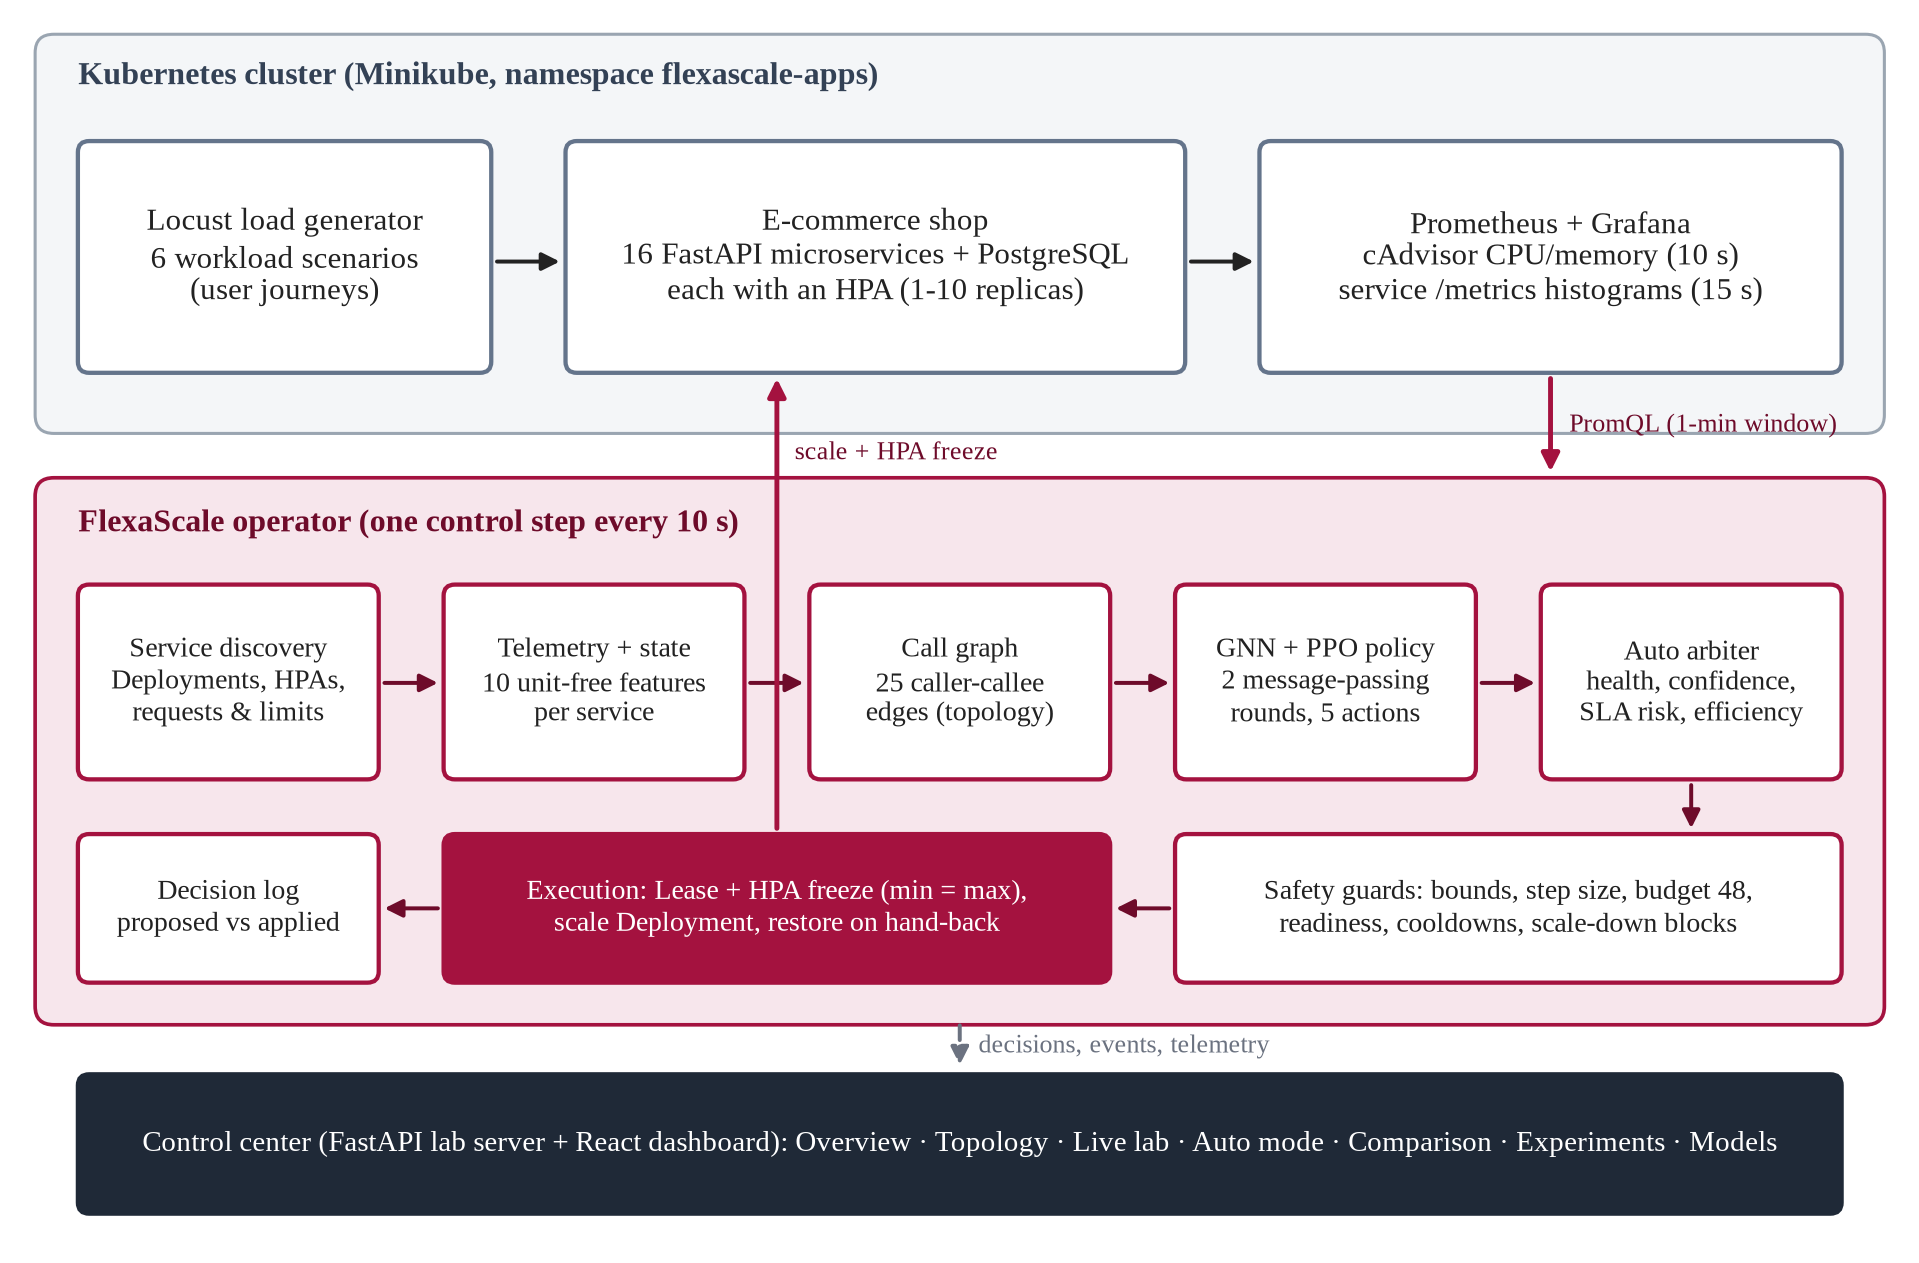
\includegraphics[width=1.0\textwidth]{figures/fig_architecture.png}
\caption{FlexaScale~system~architecture}\label{fig:arch}
\end{figure}

\subsection{Application~under~control}

The~main~test~application~is~an~e-commerce~shop~of~16~Python~(FastAPI)~microservices~with~a~React~frontend~and~a~PostgreSQL~database,~deployed~by~a~Helm~chart.~Every~service~exports~a~request~counter~and~a~latency~histogram~on~a~\texttt{/\allowbreak{}metrics}~endpoint~and~has~its~own~HPA.~Figure~\ref{fig:callgraph}~shows~the~call~graph~used~by~the~policy:~the~API~gateway~calls~nine~services~directly,~and~a~checkout~in~the~order~service~fans~out~to~catalogue,~inventory,~fraud,~payment,~shipping,~cart~and~notification~services.~A~second,~five-service~bookstore~application~is~used~to~show~that~nothing~in~FlexaScale~is~specific~to~the~shop.


\begin{figure}[!htbp]\centering
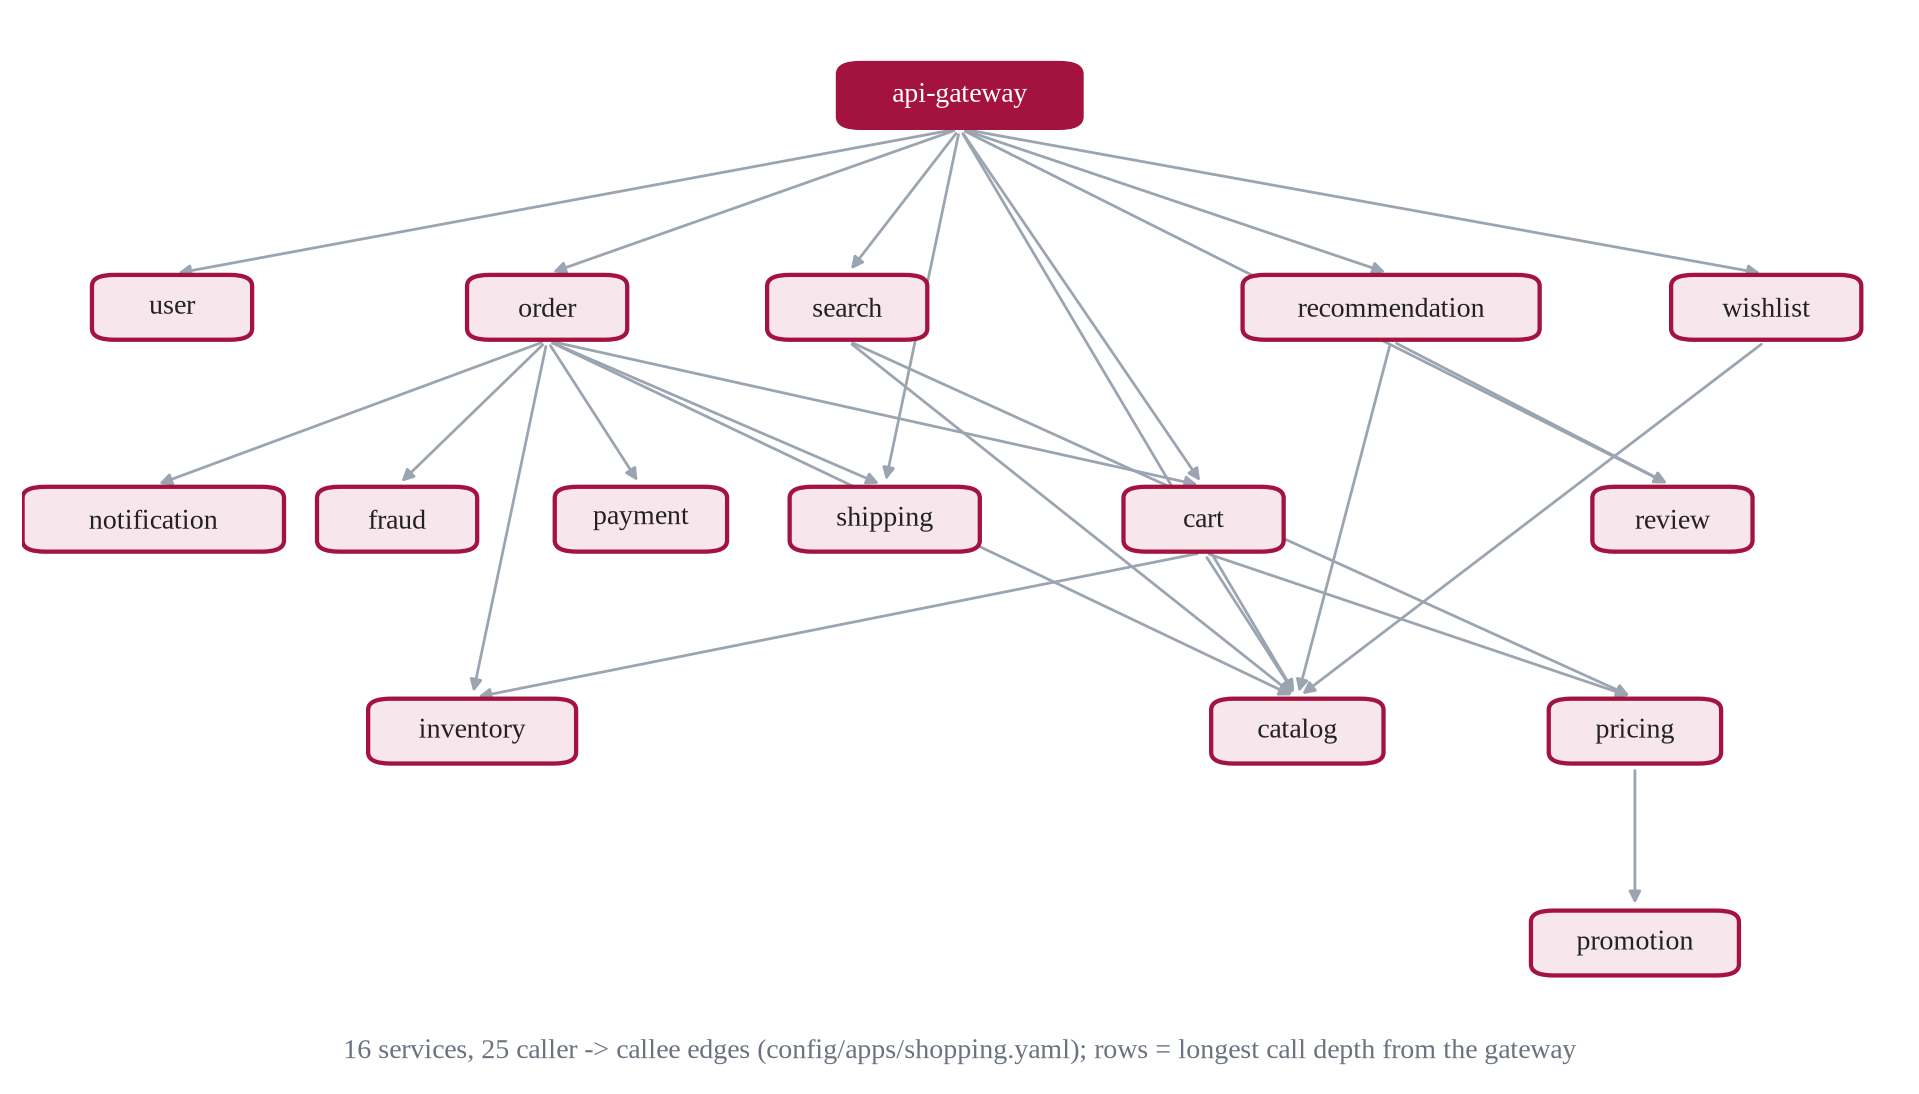
\includegraphics[width=0.85\textwidth]{figures/fig_call_graph.png}
\caption{Call~graph~of~the~16-service~shop~used~by~the~policy}\label{fig:callgraph}
\end{figure}

\subsection{Metrics~pipeline~and~service~discovery}

Prometheus~scrapes~CPU~and~memory~from~cAdvisor~every~10~seconds~and~each~service's~\texttt{/\allowbreak{}metrics}~endpoint~every~15~seconds.~At~each~step~the~operator~issues~a~handful~of~batched~PromQL~queries~over~a~one-minute~window.~Three~real-world~problems~were~found~and~handled~explicitly~while~building~this~pipeline:~cAdvisor~on~some~runtimes~reports~CPU~only~per~pod,~not~per~container;~pods~scraped~by~two~jobs~had~their~request~rates~counted~twice;~and~a~service~with~no~requests~was~being~reported~as~missing~rather~than~as~zero.~Discovery~lists~the~Deployments~carrying~the~application's~label,~finds~each~one's~HPA~by~its~scale~target~rather~than~by~name,~and~reads~requests,~limits~and~replica~counts.


\subsection{State~representation}

For~each~service,~the~operator~builds~the~ten~features~of~Table~\ref{tab:features}.~All~of~them~are~ratios~or~logarithms,~so~that~a~fast~service~and~a~slow~service,~or~a~small~cluster~and~a~large~one,~produce~comparable~numbers.~The~same~code~computes~the~features~in~the~simulator~during~training~and~in~the~operator~live,~which~removes~a~common~source~of~mismatch~between~training~and~deployment.


\begingroup\small\setlength{\tabcolsep}{4pt}\renewcommand{\arraystretch}{1.25}
\begin{longtable}{|>{\raggedright\arraybackslash}p{0.71cm}|>{\raggedright\arraybackslash}p{3.13cm}|>{\raggedright\arraybackslash}p{8.25cm}|>{\raggedright\arraybackslash}p{2.13cm}|}
\caption{The~ten~per-service~features~(observation~version~3)}\label{tab:features}\\\hline
\textbf{\#} & \textbf{Feature} & \textbf{Definition} & \textbf{Range}\\\hline\endfirsthead
\hline \textbf{\#} & \textbf{Feature} & \textbf{Definition} & \textbf{Range}\\\hline\endhead
0 & cpu\_limit\_frac & CPU~per~ready~replica~divided~by~the~CPU~limit & 0-2\\\hline
1 & cpu\_limit\_trend & Change~of~feature~0~since~the~previous~decision & $-$1~to~1\\\hline
2 & rps\_trend & Request~rate~now~divided~by~the~rate~about~60~s~earlier & 0-3\\\hline
3 & latency\_inflation & log2~of~latency~divided~by~the~service's~own~low-load~latency & $-$1~to~4\\\hline
4 & replica\_frac & Replicas~divided~by~the~maximum~(10) & 0-1\\\hline
5 & ready\_frac & Ready~replicas~divided~by~desired~replicas & 0-1\\\hline
6 & cpu\_per\_request & log10~of~CPU-milliseconds~per~request,~divided~by~3 & 0-1\\\hline
7 & burstiness & log2~of~peak~over~mean~request~rate~in~the~last~5~minutes & 0-3\\\hline
8 & since\_scale\_up & Seconds~since~the~last~scale-up~divided~by~60~(capped) & 0-1\\\hline
9 & since\_scale\_down & Seconds~since~the~last~scale-down~divided~by~60~(capped) & 0-1\\\hline
\end{longtable}\endgroup

The~observation~given~to~the~network~contains~these~features~for~up~to~20~services,~the~20~$\times$~20~adjacency~matrix~of~the~call~graph,~a~mask~marking~which~of~the~20~slots~hold~a~real~service,~and~a~one-hot~vector~marking~the~\textit{focal}~service~whose~action~is~being~decided:~640~numbers~in~total.~An~application~with~more~than~20~services~is~refused~as~incompatible.


\subsection{Policy~network}

Figure~\ref{fig:model}~shows~the~network.~Each~service's~ten~features~are~mapped~to~a~64-dimensional~embedding.~Two~rounds~of~message~passing~then~let~every~service~combine~its~own~embedding~with~the~mean~embedding~of~the~services~it~calls~and~the~mean~embedding~of~the~services~that~call~it,~with~separate~weights~for~each~direction~(Equation~\ref{eq:mp})~\cite{mpnn,gcn}.~The~focal~service's~final~embedding~is~concatenated~with~the~mean~embedding~of~the~whole~application,~and~this~128-dimensional~vector~feeds~the~PPO~actor,~which~outputs~a~probability~for~each~of~the~five~replica~changes,~and,~during~training~only,~a~critic~that~estimates~the~value~of~the~state.~The~network~has~42,566~parameters.


\begin{equation}\label{eq:mp}
h_i^{(k+1)} = h_i^{(k)} + \mathrm{ReLU}\left(\mathrm{LN}\left(W_0^{(k)} h_i^{(k)} + W_1^{(k)}\,\bar{h}^{(k)}_{\mathrm{callees}(i)} + W_2^{(k)}\,\bar{h}^{(k)}_{\mathrm{callers}(i)}\right)\right)
\end{equation}

\begin{figure}[!htbp]\centering
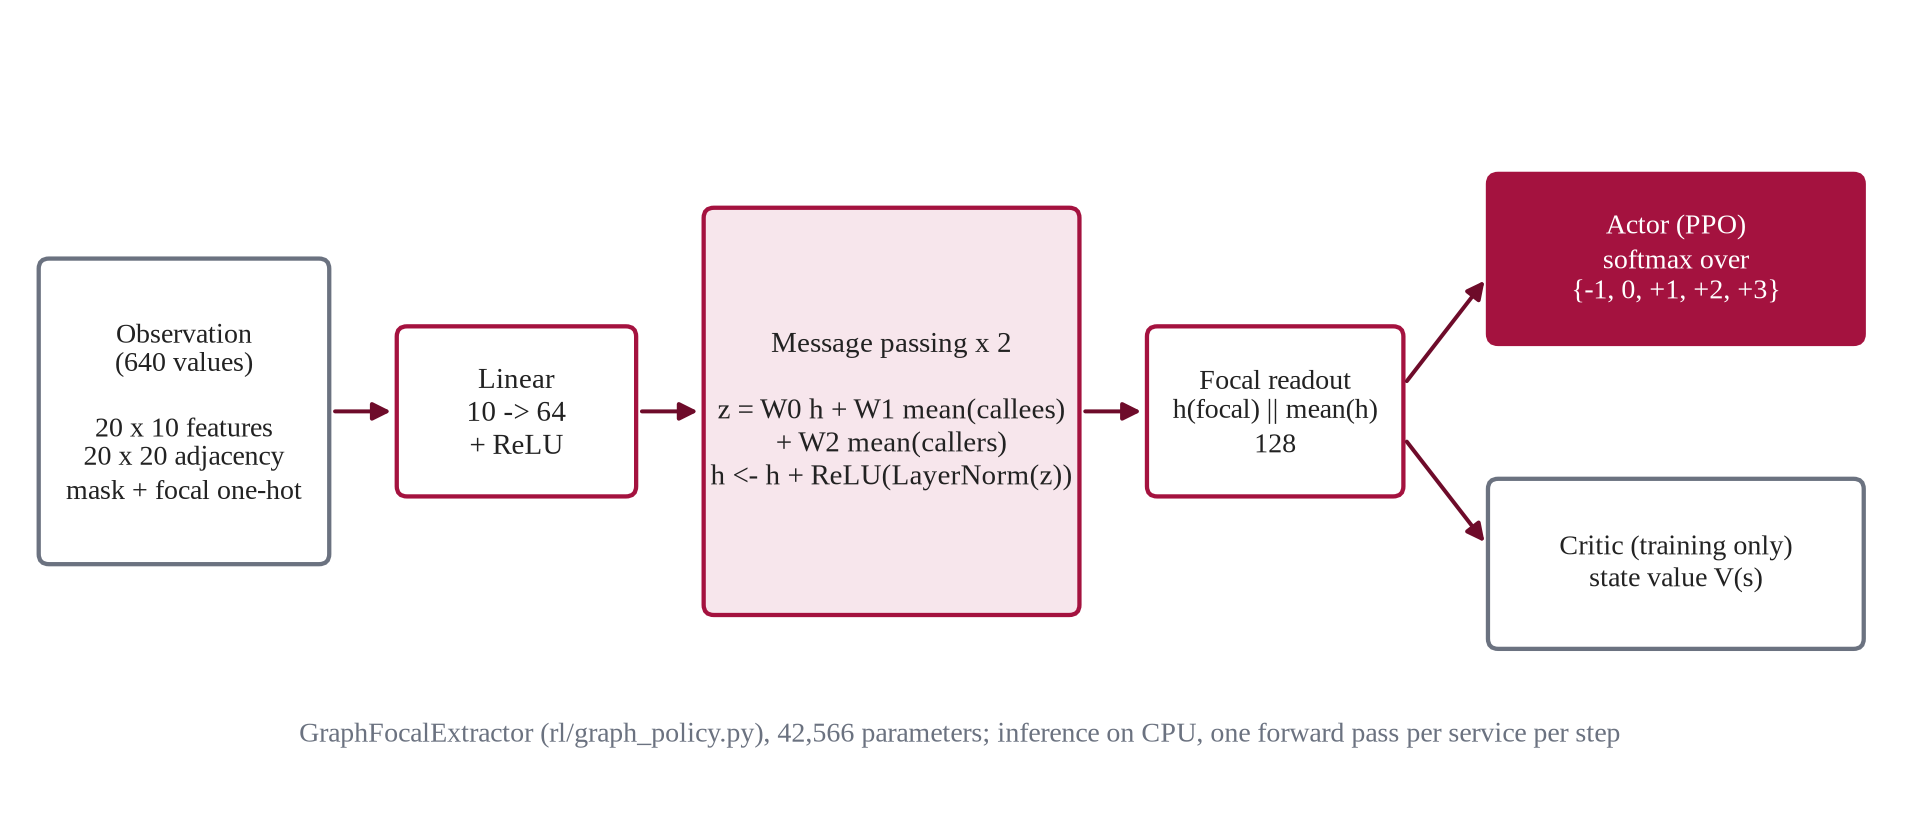
\includegraphics[width=1.0\textwidth]{figures/fig_model.png}
\caption{Graph~policy~network:~per-service~embedding,~two~rounds~of~message~passing,~focal~readout~and~PPO~heads}\label{fig:model}
\end{figure}

On~the~live~cluster~the~operator~takes~the~most~likely~action~for~each~service~and~reports~its~probability~as~the~policy's~confidence.~One~forward~pass~per~service~per~step~runs~on~the~CPU~in~milliseconds.


\subsection{Auto~mode:~per-service~arbitration}

Auto~mode~decides,~for~every~service~and~every~step,~whether~FlexaScale~or~the~native~HPA~should~be~in~charge.~Both~controllers'~proposals~are~computed~from~the~same~telemetry:~the~policy's~action,~and~the~HPA's~recommendation~from~Equation~\ref{eq:hpa}~at~a~configured~target.~Four~rules~are~then~checked~in~order~(Figure~\ref{fig:auto});~the~first~that~applies~decides.~Moving~a~service~\textit{to}~FlexaScale~requires~the~same~choice~on~two~consecutive~steps,~while~moving~it~back~to~the~HPA~for~health~or~SLA~risk~happens~immediately.~This~asymmetry~prevents~flapping~and~makes~the~safe~direction~fast.


\begin{figure}[!htbp]\centering
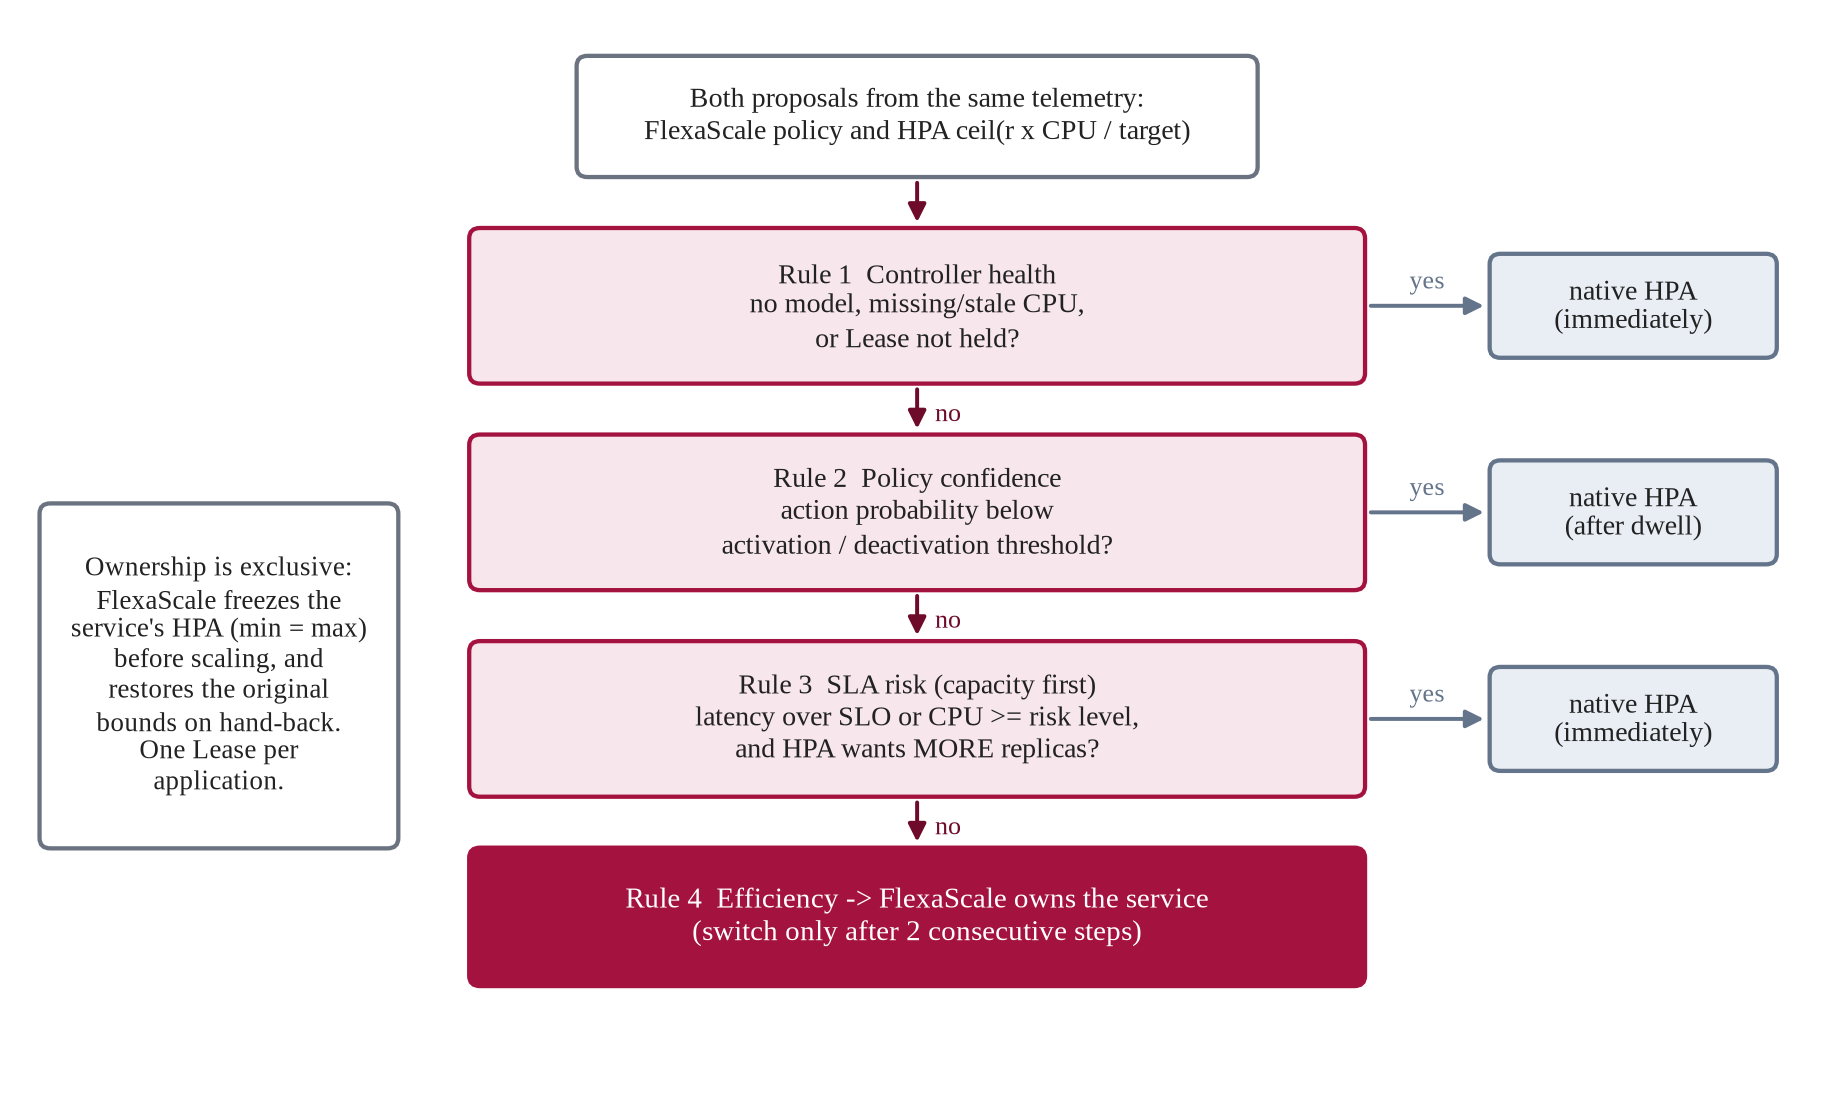
\includegraphics[width=0.85\textwidth]{figures/fig_auto_rules.png}
\caption{Auto~mode~decision~rules,~applied~per~service~every~10~s}\label{fig:auto}
\end{figure}

The~SLA-risk~rule~embodies~a~\textit{capacity~first}~principle:~when~a~service~is~at~risk,~the~controller~that~wants~more~replicas~wins.~In~the~shop's~default~policy~the~CPU~risk~level~is~400\%~of~the~request~(80\%~of~the~limit)~and~the~HPA~recommendation~is~computed~at~a~target~of~350\%,~the~tuned~value~found~on~the~second~laptop.~The~confidence~thresholds~of~rule~2~are~set~to~zero~in~the~shop's~policy,~so~that~rule~never~fires~there;~Section~5.1.8~explains~why.


\subsection{Safety~layer~and~exclusive~ownership}

Every~proposal~passes~the~guards~of~Table~\ref{tab:guards}~before~it~can~reach~the~cluster.~A~guard~can~reduce~or~block~a~change,~never~enlarge~it,~and~every~decision~records~either~\texttt{accepted}~or~the~reasons~it~was~changed.


\begingroup\small\setlength{\tabcolsep}{4pt}\renewcommand{\arraystretch}{1.25}
\begin{longtable}{|>{\raggedright\arraybackslash}p{3.71cm}|>{\raggedright\arraybackslash}p{11.14cm}|}
\caption{Safety~guards~applied~to~every~proposal}\label{tab:guards}\\\hline
\textbf{Guard} & \textbf{Rule~in~the~shop's~policy}\\\hline\endfirsthead
\hline \textbf{Guard} & \textbf{Rule~in~the~shop's~policy}\\\hline\endhead
Bounds & Never~below~the~service's~minimum~(1)~or~above~its~maximum~(10)\\\hline
Step~size & At~most~+3~replicas~up~and~$-$1~down~per~step\\\hline
Replica~budget & At~most~48~replicas~for~the~whole~application,~so~the~node~is~not~overloaded\\\hline
Readiness & No~scale-up~while~new~pods~are~still~starting;~no~scale-down~while~pods~are~not~ready\\\hline
Cooldowns & 20~s~after~a~scale-up~and~30~s~after~a~scale-down,~so~telemetry~can~catch~up\\\hline
Scale-down~blocks & No~scale-down~while~CPU~$\ge$~400\%~of~request,~memory~$\ge$~90\%~or~latency~above~the~SLO\\\hline
Telemetry & Missing~or~stale~CPU~(older~than~120~s):~no~FlexaScale~decision;~the~service~goes~to~its~HPA\\\hline
Ownership & Act~only~while~holding~the~application's~Lease~and~after~freezing~the~service's~HPA\\\hline
\end{longtable}\endgroup

Ownership~is~enforced~with~two~Kubernetes~mechanisms~(Figure~\ref{fig:own}).~First,~in~live~mode~the~operator~must~hold~a~\texttt{coordination.\allowbreak{}k8s.\allowbreak{}io}~Lease~named~after~the~application;~it~is~renewed~every~step~and~expires~after~30~seconds,~so~only~one~FlexaScale~controller~can~act~on~an~application.~Second,~before~FlexaScale~changes~a~service,~it~sets~that~service's~HPA~to~\texttt{minReplicas~=~maxReplicas}~equal~to~the~new~count~and~stores~the~original~bounds~in~annotations~on~the~HPA.~A~frozen~HPA~cannot~move~the~replicas,~so~the~two~controllers~never~act~on~the~same~Deployment~at~once.~Hand-back~restores~the~original~bounds~from~the~annotations.~Hand-back~happens~per~service~(Auto~rule,~missing~telemetry)~or~for~all~services~(operator~stop,~a~failed~step,~a~lost~Lease,~shutdown),~and~the~experiment~lab~adds~a~watchdog~that~restores~every~HPA~itself~if~the~operator~process~dies~or~stops~updating~its~status~for~four~poll~intervals.


\begin{figure}[!htbp]\centering
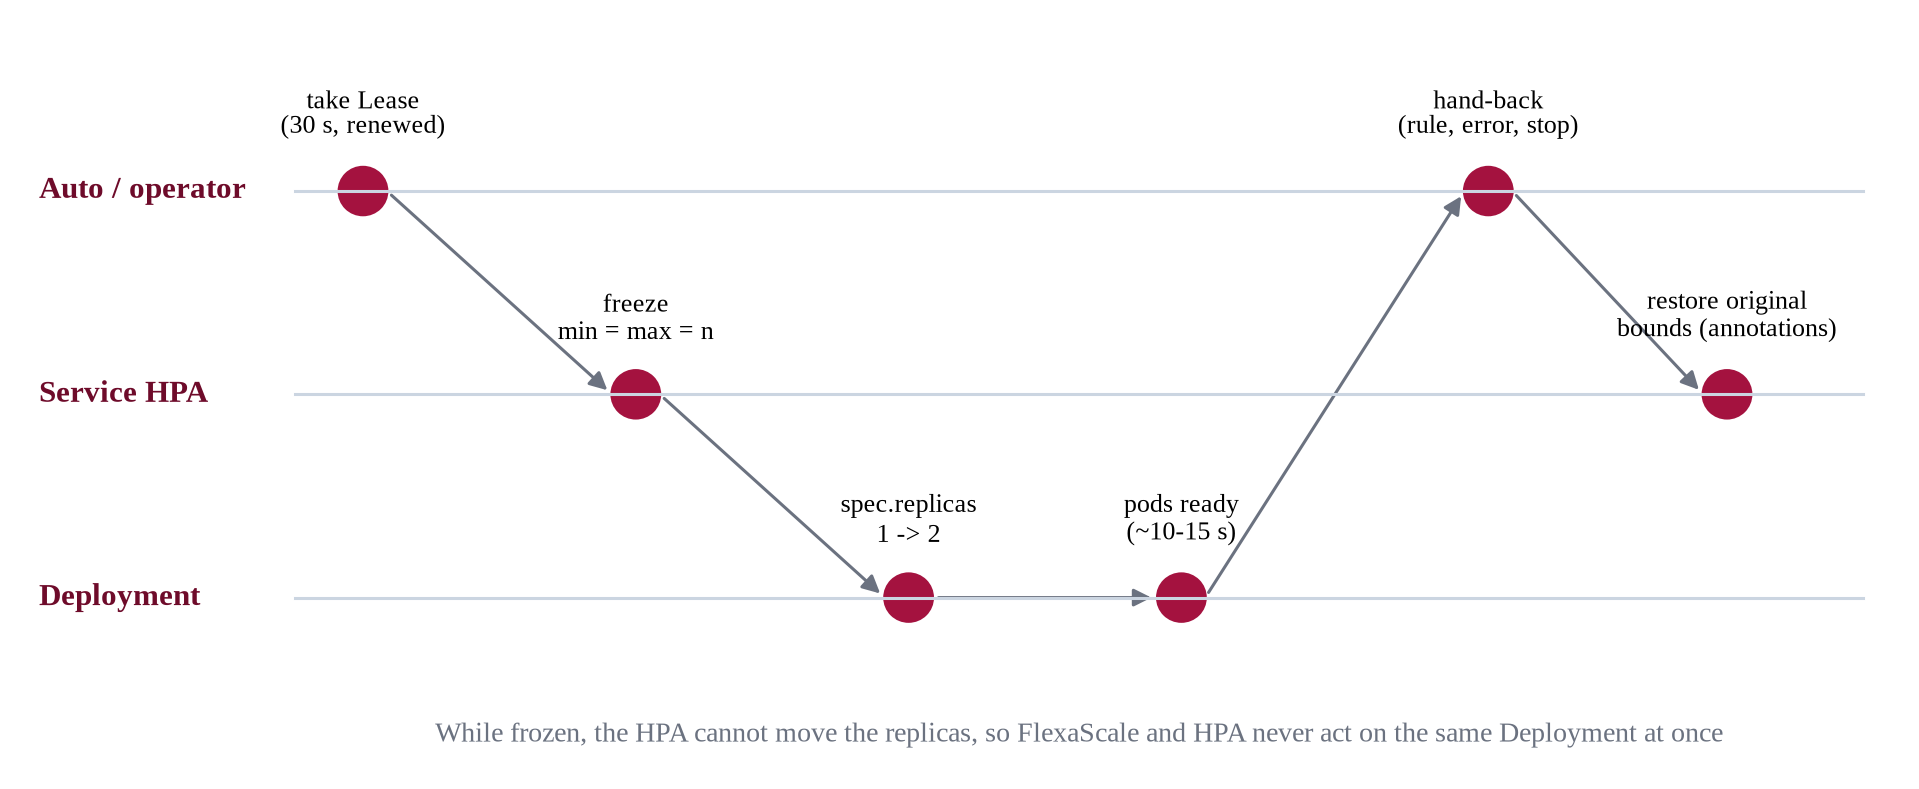
\includegraphics[width=1.0\textwidth]{figures/fig_ownership.png}
\caption{Ownership~sequence:~Lease,~HPA~freeze,~scaling~and~hand-back}\label{fig:own}
\end{figure}

\subsection{Control~center~and~packaging}

The~control~center~is~a~FastAPI~lab~server,~bound~to~the~local~machine~only,~with~a~React~and~TypeScript~dashboard.~Its~seven~pages~are~Overview,~Service~topology,~Live~lab,~Auto~mode,~Comparison,~Experiments~and~Models.~The~Live~lab~starts~a~run~in~one~of~three~modes~(native~HPA~with~FlexaScale~in~shadow,~FlexaScale,~Auto)~and~shows~a~live~autoscaling~timeline~of~desired~and~ready~replicas,~both~controllers'~proposals,~owner~bands,~traffic~and~latency.~A~single~command~(\texttt{.\allowbreak{}/\allowbreak{}fsctl~start})~brings~up~the~cluster,~port-forwards,~checks~and~the~dashboard;~\texttt{.\allowbreak{}/\allowbreak{}fsctl~stop}~stops~everything~and~verifies~that~every~HPA~has~been~restored.~For~installation~into~a~cluster,~the~operator~is~packaged~as~a~Helm~chart.~Its~namespaced~Role~grants~only~read~access~in~observe~mode;~the~write~verbs~(patching~HPAs~and~Deployments,~updating~the~scale~sub-resource~and~the~Lease)~are~granted~only~when~the~release~is~installed~in~live~mode.~A~Helm~hook~hands~every~service~back~to~its~HPA~before~an~upgrade,~a~rollback~or~an~uninstall.


\subsection{Relation~to~the~Phase~2~design}

The~implementation~follows~the~six-component~architecture~approved~in~the~design~phase.~Four~points~changed~during~implementation,~for~the~reasons~given~in~Table~\ref{tab:deviations}.


\begingroup\small\setlength{\tabcolsep}{4pt}\renewcommand{\arraystretch}{1.25}
\begin{longtable}{|>{\raggedright\arraybackslash}p{3.49cm}|>{\raggedright\arraybackslash}p{4.65cm}|>{\raggedright\arraybackslash}p{6.40cm}|}
\caption{Differences~between~the~Phase~2~design~and~the~implemented~system}\label{tab:deviations}\\\hline
\textbf{Design~element} & \textbf{What~was~implemented} & \textbf{Reason}\\\hline\endfirsthead
\hline \textbf{Design~element} & \textbf{What~was~implemented} & \textbf{Reason}\\\hline\endhead
Adaptive~reward~weighting~by~traffic~phase & A~fixed,~multi-term~reward~with~documented~weights~(Equation~\ref{eq:reward}) & Weights~changing~with~a~detected~phase~made~training~targets~non-stationary~and~results~hard~to~attribute;~the~fixed~reward~already~charges~latency~inflation,~SLO~violation,~failures,~replicas~and~churn.\\\hline
Confidence-based~delegation~to~HPA & Implemented~as~Auto~rule~2;~thresholds~set~to~0~in~the~shop's~policy & The~policy's~action~probabilities~were~not~calibrated~as~a~measure~of~correctness;~health~and~SLA-risk~rules~gave~clearer,~testable~hand-back~conditions.\\\hline
Online~PPO~updates~on~the~live~cluster & Offline~training~in~a~fitted~twin;~inference~only~on~the~cluster & Learning~on~a~live~application~is~slow~and~risky;~a~policy~that~changes~during~an~experiment~cannot~be~evaluated~fairly.\\\hline
Three-node~cloud~staging~cluster & Single-node~Minikube~on~two~laptops & Zero~cost~and~full~control~of~the~environment;~the~limitation~on~load~is~reported~in~Section~6.6.\\\hline
\end{longtable}\endgroup

\section{Proposed~approach~and~procedure}

This~section~explains~how~the~policy~is~obtained~and~how~the~system~operates,~step~by~step,~in~enough~detail~to~reproduce~the~work.~Figure~\ref{fig:training}~summarises~the~training~pipeline~and~Figure~\ref{fig:loop}~the~live~control~loop.


\subsection{Step~1:~Simulation~environments}

Training~on~the~real~cluster~would~take~months~and~could~break~the~application,~so~every~policy~was~trained~in~simulation.~Two~generations~of~simulator~were~used.~Versions~v1~to~v6~used~Gymnasium~environments~driven~by~the~Alibaba~trace,~in~which~each~service's~load~followed~a~trace~segment.~Live~tests~showed~that~these~policies~did~not~transfer~well:~they~had~never~seen~the~shop,~and~the~earlier~simulators~made~the~HPA's~rule~close~to~optimal~by~construction.


Versions~v7~and~v9~were~therefore~trained~in~an~\textit{application~twin},~a~simulator~fitted~to~measurements~of~our~own~shop.~The~twin~models~each~service's~CPU~cost~per~request,~its~0.5-core~CPU~limit~and~the~queueing~that~follows~when~the~limit~is~reached,~the~call~graph,~pod~start-up~time~(median~10~s,~90th~percentile~15~s,~measured~live),~and~controllers~that~see~delayed~metrics~as~the~real~ones~do.~One~step~is~10~seconds.~Training~workloads~are~random~variations~of~the~six~live~scenarios~with~8~to~45~peak~users~and~durations~of~300~to~600~seconds,~and~a~quarter~of~the~episodes~use~a~randomly~generated~application~so~that~the~policy~must~read~the~graph~instead~of~memorising~service~names.~The~v9~twin,~fitted~to~the~second~laptop,~reproduces~the~calibration~runs~with~a~mean~absolute~error~of~2.0\%~in~replica-hours~and~8.9\%~in~p95~latency~(Figure~\ref{fig:twin}).


\begin{figure}[!htbp]\centering
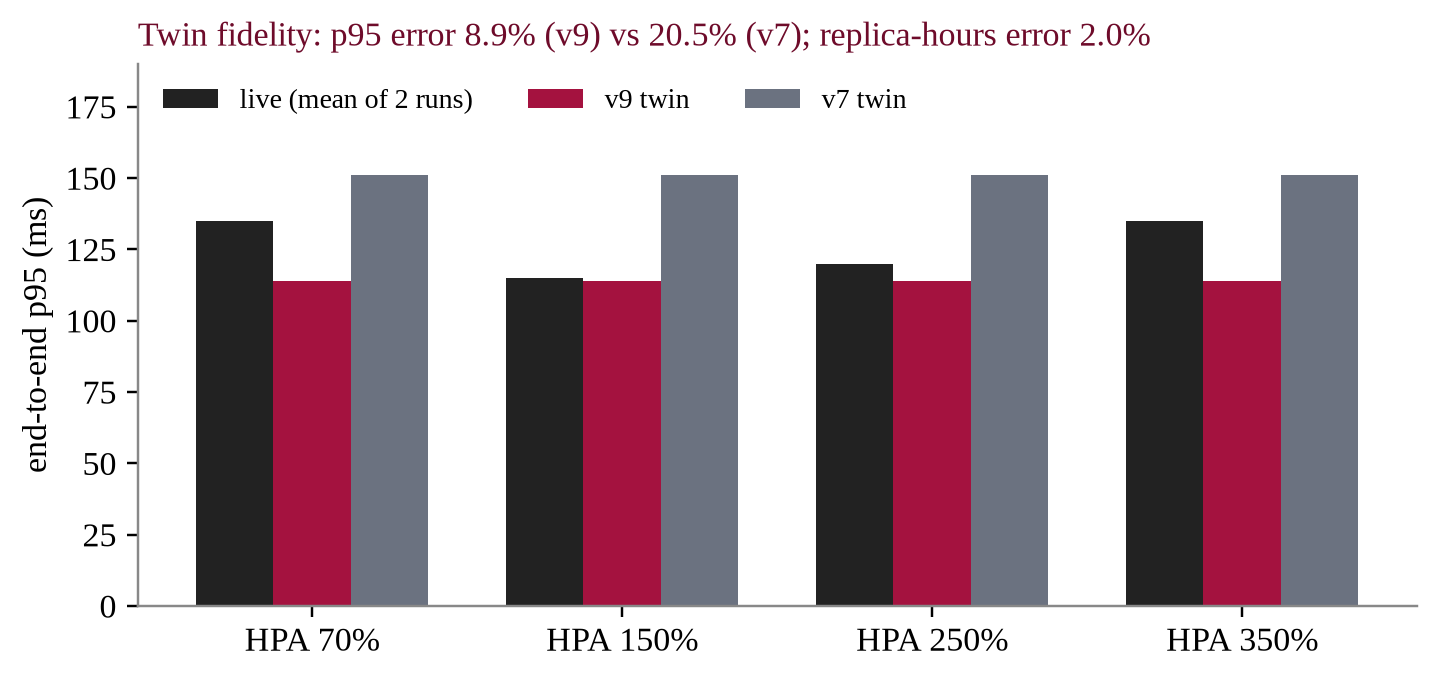
\includegraphics[width=0.7\textwidth]{figures/fig_twin_check.png}
\caption{Twin~fidelity~against~live~calibration~runs~on~the~second~laptop~(p95~latency)}\label{fig:twin}
\end{figure}

\subsection{Step~2:~Reward~function}

The~reward~is~computed~per~10-second~step~in~units~of~replica-equivalents,~so~that~each~weight~answers~a~concrete~question,~such~as~how~many~extra~replicas~avoiding~an~SLO~violation~is~worth~(Equation~\ref{eq:reward}).~The~first~term~counts~replicas~above~each~service's~minimum;~the~second~charges~the~inflation~of~end-to-end~p95~latency~over~its~value~with~ample~capacity,~capped~at~four;~\textit{v}~is~the~fraction~of~the~step~in~which~p95~exceeded~1000~ms,~\textit{f}~the~percentage~of~failed~requests~and~\textit{c}~the~number~of~replica~changes~(churn).


\begin{equation}\label{eq:reward}
R_t = -0.1\left(\sum_i (r_i - r_i^{\min}) + 6\,\min\left(4, \frac{p95_t}{p95^{0}} - 1\right) + 10\,v_t + 5\,f_t + 0.25\,c_t\right)
\end{equation}

For~example,~a~step~with~three~extra~replicas,~no~slowdown~and~one~change~scores~$-$0.325,~while~a~step~with~no~extra~replicas~but~doubled~latency~and~the~SLO~broken~for~half~the~step~scores~$-$1.1,~so~the~learner~prefers~paying~for~the~replicas.


\subsection{Step~3:~Warm~start~by~imitation}

Early~versions~trained~with~PPO~from~scratch~learned~to~scale~everything~up,~or~failed~to~match~a~simple~threshold~rule~that~the~network~could~represent~exactly.~From~v5~onward,~each~run~therefore~starts~by~imitating~a~rule~(behaviour~cloning:~cross-entropy~on~the~rule's~actions,~with~the~critic~fitted~to~returns).~The~teacher~for~v7~and~v9~was~chosen~from~the~family~\texttt{limit\_\allowbreak{}target(t/\allowbreak{}d)},~which~scales~up~when~CPU~per~replica~exceeds~a~fraction~\textit{t}~of~the~limit~and~down~below~\textit{d},~with~\textit{t}~$\in$~\{0.4,~0.5,~0.6,~0.7\}~and~\textit{d}~$\in$~\{0.2,~0.3\};~the~validation-best~rule~was~\texttt{limit\_\allowbreak{}target(0.\allowbreak{}6/\allowbreak{}0.\allowbreak{}3)}.


\subsection{Step~4:~PPO~fine-tuning}

PPO~\cite{ppo}~improves~the~policy~by~maximising~the~clipped~surrogate~objective~of~Equation~\ref{eq:ppo},~where~$\rho$~is~the~ratio~of~the~new~to~the~old~probability~of~the~action~taken~and~\^{A}~is~the~advantage~estimated~with~generalised~advantage~estimation~(Equation~\ref{eq:gae})~\cite{gae}.~The~clip~keeps~each~update~close~to~the~previous~policy,~which~keeps~training~stable.~The~implementation~uses~Stable-Baselines3~\cite{sb3}~with~the~settings~in~Table~\ref{tab:hyper}.


\begin{equation}\label{eq:ppo}
L(\theta) = \hat{E}_t\left[\min\left(\rho_t(\theta)\,\hat{A}_t,\ \mathrm{clip}(\rho_t(\theta), 1-\epsilon, 1+\epsilon)\,\hat{A}_t\right)\right]
\end{equation}

\begin{equation}\label{eq:gae}
\hat{A}_t = \sum_{l=0}^{\infty} (\gamma\lambda)^l\,\delta_{t+l}, \qquad \delta_t = R_t + \gamma V(s_{t+1}) - V(s_t)
\end{equation}

\begingroup\small\setlength{\tabcolsep}{4pt}\renewcommand{\arraystretch}{1.25}
\begin{longtable}{|>{\raggedright\arraybackslash}p{4.41cm}|>{\raggedright\arraybackslash}p{2.70cm}|>{\raggedright\arraybackslash}p{4.41cm}|>{\raggedright\arraybackslash}p{2.70cm}|}
\caption{Training~hyperparameters~(v7~and~v9~protocol)}\label{tab:hyper}\\\hline
\textbf{Parameter} & \textbf{Value} & \textbf{Parameter} & \textbf{Value}\\\hline\endfirsthead
\hline \textbf{Parameter} & \textbf{Value} & \textbf{Parameter} & \textbf{Value}\\\hline\endhead
Algorithm & PPO~(Stable-Baselines3) & Discount~$\gamma$ & 0.97\\\hline
Parallel~decisions~per~step & 4~simulations~$\times$~20~service~agents & GAE~$\lambda$ & 0.95\\\hline
Rollout~length & 64~steps~$\times$~80~agents~=~5,120~decisions & Entropy~coefficient & 0.01\\\hline
Mini-batch~size & 512 & Value-loss~coefficient & 0.5\\\hline
Epochs~per~update & 10 & Max~gradient~norm & 0.5\\\hline
Learning~rate~(from~scratch~/~after~warm~start) & 3~$\times$~10\textsuperscript{$-$}\textsuperscript{4}~/~1~$\times$~10\textsuperscript{$-$}\textsuperscript{4} & Clip~range~(from~scratch~/~after~warm~start) & 0.2~/~0.1\\\hline
Target~KL~(after~warm~start) & 0.02 & Agent-steps~per~run & 2,000,000\\\hline
Hidden~size,~message-passing~rounds & 64,~2 & Actor~/~critic~heads & 64~/~64~units\\\hline
Seeds & 1~and~2 & Validation & every~250,000~steps~on~40~fixed~workloads\\\hline
\end{longtable}\endgroup

A~measured~profile~showed~that~the~PPO~update,~not~the~simulator,~dominated~training~time~(77-84\%~of~each~iteration~on~the~CPU),~so~a~rule~was~fixed~in~advance:~train~on~the~GPU~only~if~it~was~at~least~1.5~times~faster.~The~RTX~3050~was~1.79~times~faster~than~the~best~CPU~setting,~and~the~four~v9~runs~of~2,000,000~agent-steps~each~took~about~63~minutes~in~total.~The~device~changed~only~the~speed,~never~the~protocol,~seeds~or~selection.


\begin{figure}[!htbp]\centering
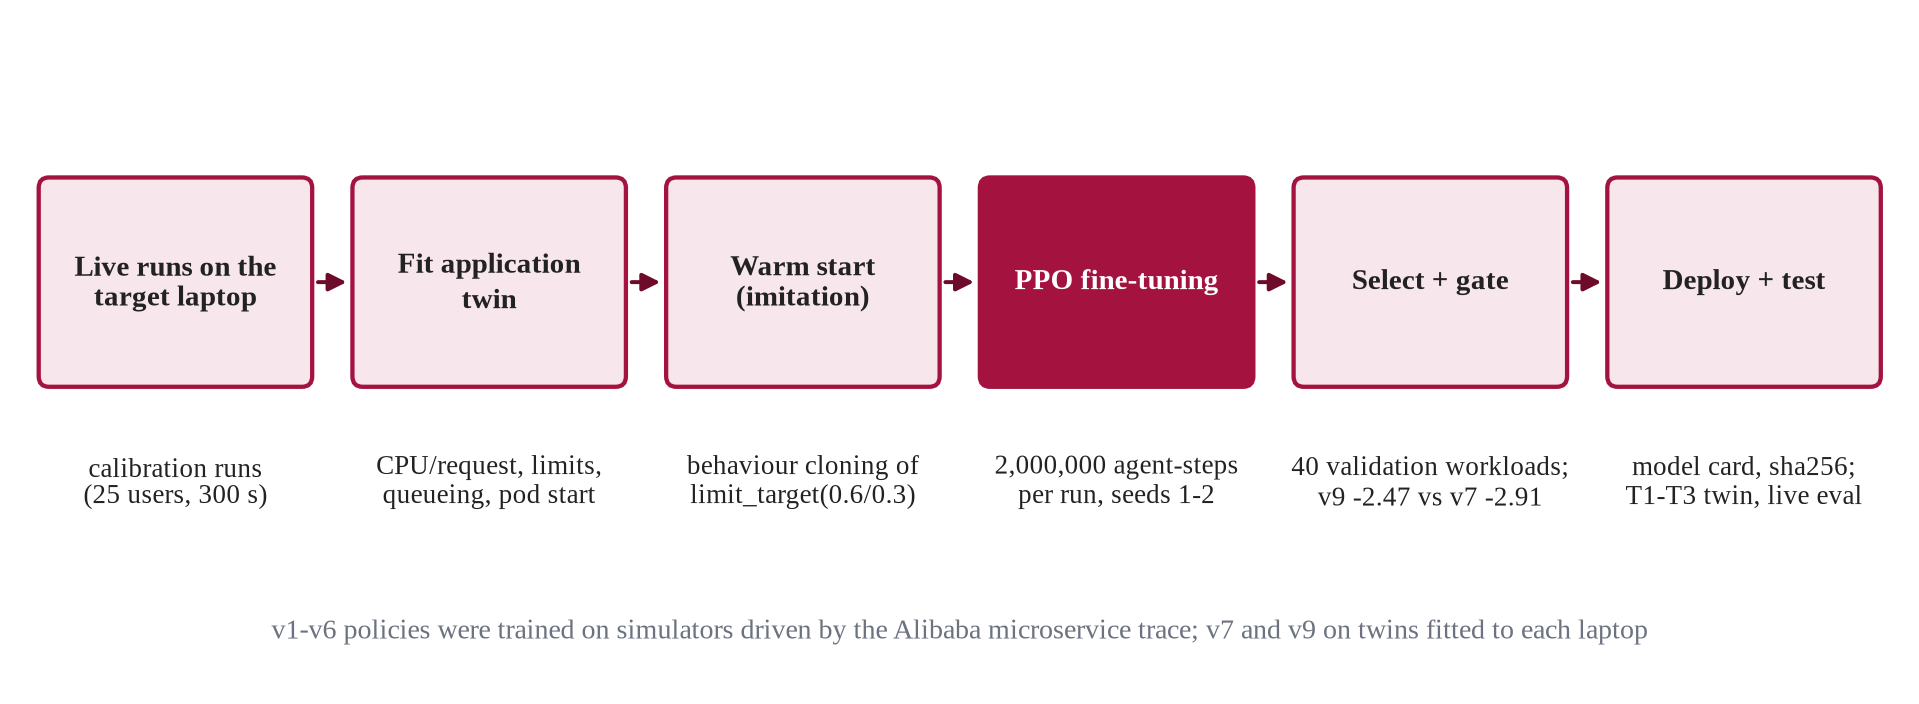
\includegraphics[width=1.0\textwidth]{figures/fig_training.png}
\caption{Training~pipeline~of~the~v7~and~v9~policies}\label{fig:training}
\end{figure}

\subsection{Step~5:~Selection,~gate~and~model~card}

Each~run~was~evaluated~on~40~fixed~validation~workloads~every~250,000~steps,~and~the~best~checkpoint~of~each~run~kept.~The~run~with~the~best~validation~reward~was~selected,~and~it~became~the~deployed~policy~only~if~it~passed~a~gate~against~its~predecessor.~Figure~\ref{fig:validation}~shows~the~v9~candidates:~the~selected~run~\texttt{focal\_\allowbreak{}bc\_\allowbreak{}s2}~scored~$-$2.466,~better~than~the~no-graph~variant,~the~teacher~rule~and~the~other~seed,~and~it~passed~the~gate~against~v7~($-$2.47~against~$-$2.91).~Because~selection~and~gate~used~the~same~validation~set,~the~margin~is~optimistic;~the~held-out~test~sets~in~Chapter~6~are~the~fair~comparison.~The~selected~model~is~stored~with~a~model~card~that~records~its~features,~actions,~reward,~guards,~training~runs~and~its~SHA-256~fingerprint,~and~no~earlier~model~was~overwritten.


\begin{figure}[!htbp]\centering
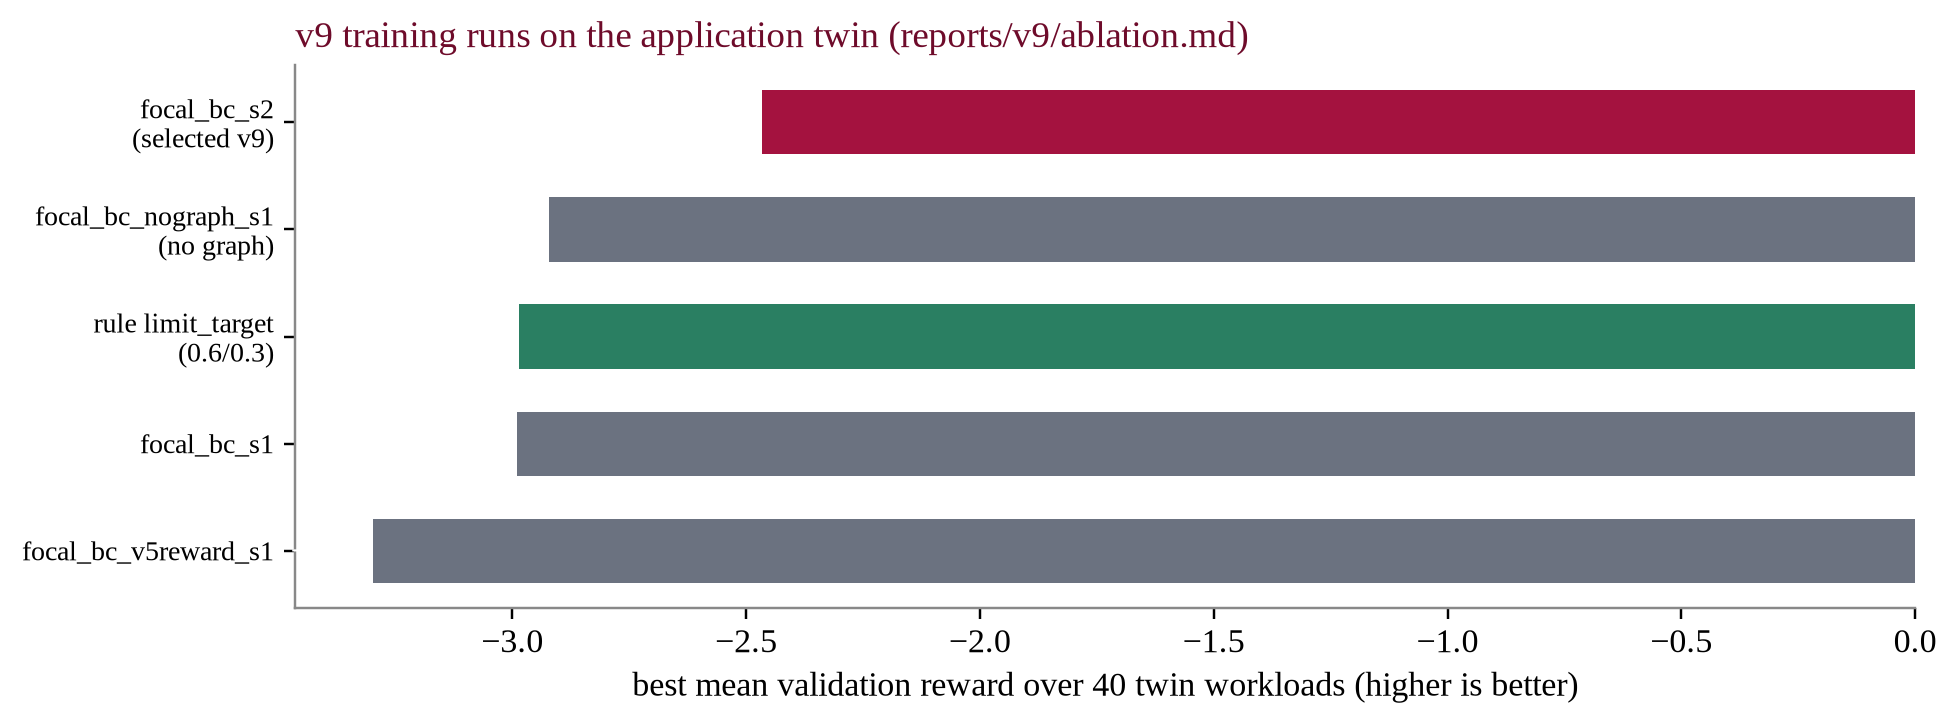
\includegraphics[width=0.8\textwidth]{figures/fig_validation.png}
\caption{Validation~reward~of~the~v9~training~runs~and~the~teacher~rule}\label{fig:validation}
\end{figure}

\subsection{Step~6:~Live~control~loop}

Algorithm~5.1~gives~one~operator~step.~It~runs~every~10~seconds~for~the~whole~application,~and~Figure~\ref{fig:loop}~shows~the~same~loop~as~a~flow.


\begin{figure}[!htbp]\centering\small
\begin{tabular}{@{}r@{\hspace{8pt}}p{0.86\textwidth}@{}}\hline
\multicolumn{2}{@{}l}{\textbf{Algorithm 5.1: FlexaScale~operator~step~(every~10~s)}}\\\hline
{\scriptsize 1} & \hspace*{0.0em}\textbf{input:}~policy~file~\textit{P},~trained~policy~$\pi$,~Lease~\textit{L},~mode~$\in$~\{observe,~live\},~Auto~on/off\\
{\scriptsize 2} & \hspace*{0.0em}discover~services~\textit{S}~and~their~HPAs~(label~selector~of~\textit{P})\\
{\scriptsize 3} & \hspace*{0.0em}query~Prometheus~once~for~all~\textit{s}~$\in$~\textit{S}~(1-minute~window);~mark~missing~or~stale~telemetry\\
{\scriptsize 4} & \hspace*{0.0em}\textbf{if}~mode~=~live~\textbf{then}~renew~\textit{L};~\textbf{if}~renewal~fails~\textbf{then}~restore~all~HPAs,~mode~$\leftarrow$~observe\\
{\scriptsize 5} & \hspace*{0.0em}\textbf{for~each}~\textit{s}~$\in$~\textit{S}~\textbf{do}~\textit{x}(\textit{s})~$\leftarrow$~FeatureTracker.update(\textit{s})\\
{\scriptsize 6} & \hspace*{0.0em}(\textit{a}(\textit{s}),~\textit{c}(\textit{s}))~$\leftarrow$~$\pi$(\textit{x},~call~graph,~focal~=~\textit{s})~for~every~\textit{s}\\
{\scriptsize 7} & \hspace*{0.0em}\textbf{for~each}~service~\textit{s}~\textbf{do}\\
{\scriptsize 8} & \hspace*{1.2em}\textit{h}(\textit{s})~$\leftarrow$~$\lceil$\textit{r}(\textit{s})~$\cdot$~CPU(\textit{s})~/~target$\rceil$~(bounded)\\
{\scriptsize 9} & \hspace*{1.2em}owner~$\leftarrow$~Auto(\textit{s},~\textit{a}(\textit{s}),~\textit{c}(\textit{s}),~\textit{h}(\textit{s}))~\textbf{if}~Auto~\textbf{else}~FlexaScale\\
{\scriptsize 10} & \hspace*{1.2em}\textbf{if}~owner~=~HPA~\textbf{then}~restore~the~HPA's~original~bounds;~log;~\textbf{continue}\\
{\scriptsize 11} & \hspace*{1.2em}\textit{n}~$\leftarrow$~guards(\textit{r}(\textit{s})~+~\textit{a}(\textit{s}))~~~(bounds,~step,~budget,~readiness,~cooldowns,~blocks)\\
{\scriptsize 12} & \hspace*{1.2em}\textbf{if}~mode~=~live~\textbf{and}~\textit{n}~$\neq$~\textit{r}(\textit{s})~\textbf{then}~freeze~HPA~at~\textit{n};~scale~Deployment~to~\textit{n}\\
{\scriptsize 13} & \hspace*{1.2em}log~proposal,~approved~count,~owner,~rule,~safety~reasons,~applied~flag\\
{\scriptsize 14} & \hspace*{0.0em}write~status~file~(heartbeat~for~the~lab~watchdog)\\
\hline\end{tabular}
\end{figure}

\begin{figure}[!htbp]\centering
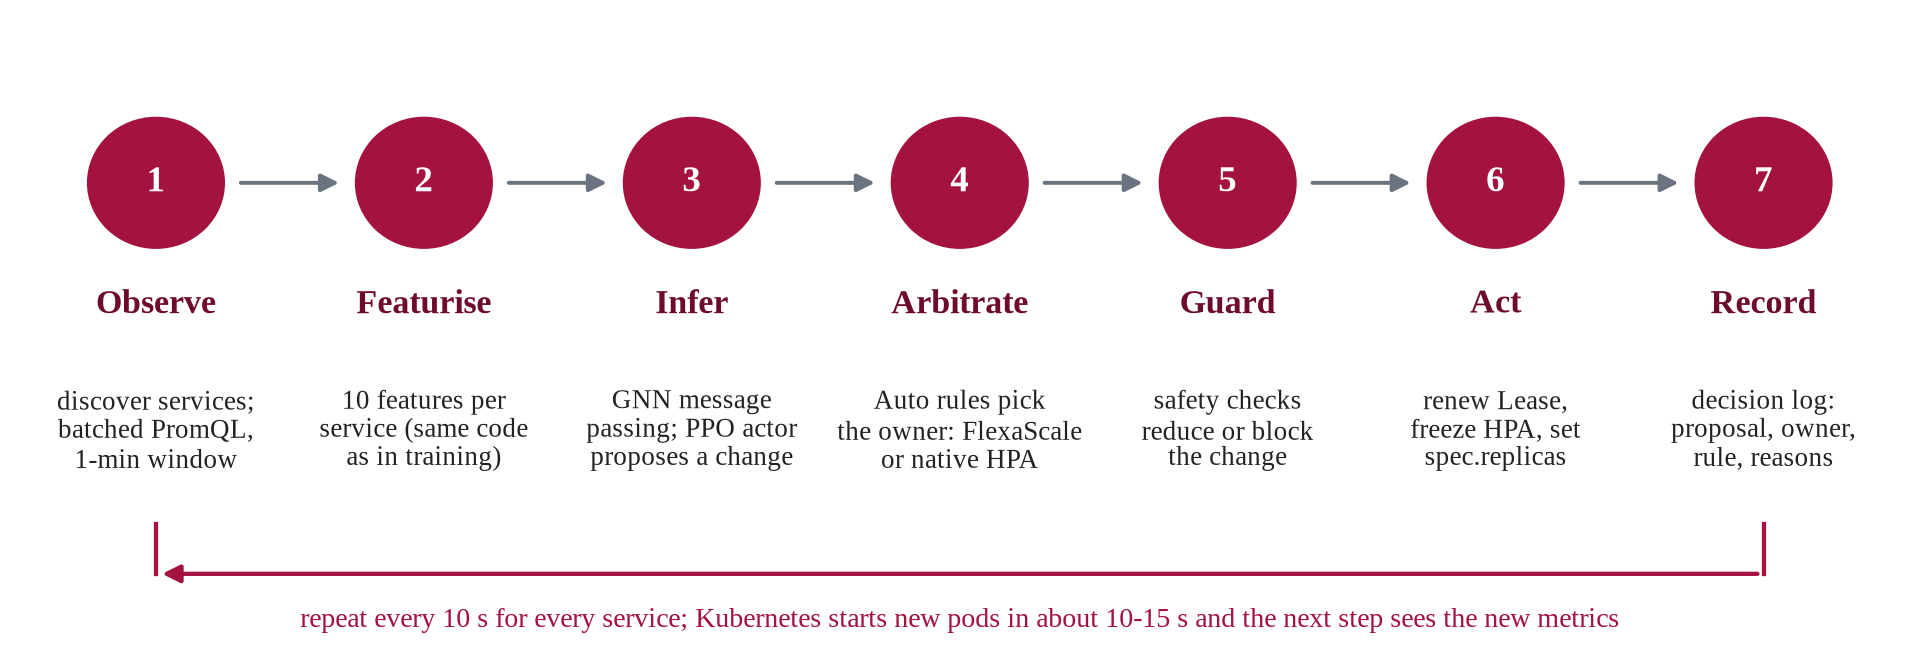
\includegraphics[width=1.0\textwidth]{figures/fig_control_loop.png}
\caption{The~live~control~loop}\label{fig:loop}
\end{figure}

\subsection{Step~7:~Auto~arbitration}

Algorithm~5.2~details~the~per-service~decision~of~Auto~mode.~The~dwell~counter~is~kept~per~service~across~steps.


\begin{figure}[!htbp]\centering\small
\begin{tabular}{@{}r@{\hspace{8pt}}p{0.86\textwidth}@{}}\hline
\multicolumn{2}{@{}l}{\textbf{Algorithm 5.2: Auto~arbitration~for~one~service}}\\\hline
{\scriptsize 1} & \hspace*{0.0em}\textbf{input:}~service~\textit{s},~current~owner~\textit{o},~policy~proposal~\textit{f},~confidence~\textit{c},~HPA~recommendation~\textit{h},~telemetry\\
{\scriptsize 2} & \hspace*{0.0em}\textbf{if}~no~model~\textbf{or}~CPU~missing/stale~\textbf{or}~Lease~not~held~\textbf{then~return}~HPA~(rule:~controller\_health)\\
{\scriptsize 3} & \hspace*{0.0em}$\theta$~$\leftarrow$~activation~threshold~\textbf{if}~\textit{o}~=~HPA~\textbf{else}~deactivation~threshold\\
{\scriptsize 4} & \hspace*{0.0em}\textbf{if}~\textit{c}~<~$\theta$~\textbf{then}~\textit{candidate}~$\leftarrow$~HPA~(rule:~policy\_confidence)\\
{\scriptsize 5} & \hspace*{0.0em}\textbf{else~if}~(latency~>~SLO~\textbf{or}~CPU~$\ge$~risk~level)~\textbf{and}~\textit{h}~>~\textit{f}~\textbf{then~return}~HPA~(rule:~sla\_risk)\\
{\scriptsize 6} & \hspace*{0.0em}\textbf{else}~\textit{candidate}~$\leftarrow$~FlexaScale~(rule:~efficiency)\\
{\scriptsize 7} & \hspace*{0.0em}\textbf{if}~\textit{candidate}~=~\textit{o}~\textbf{then}~dwell~$\leftarrow$~0;~\textbf{return}~\textit{o}\\
{\scriptsize 8} & \hspace*{0.0em}dwell~$\leftarrow$~dwell~+~1\\
{\scriptsize 9} & \hspace*{0.0em}\textbf{if}~dwell~$\ge$~2~\textbf{then}~dwell~$\leftarrow$~0;~\textbf{return}~\textit{candidate}\\
{\scriptsize 10} & \hspace*{0.0em}\textbf{return}~\textit{o}~~~(stay~with~the~current~owner~until~the~choice~is~confirmed)\\
\hline\end{tabular}
\end{figure}

\subsection{Step~8:~Experiment~procedure}

Every~experiment,~whether~a~benchmark~pair~or~a~demonstration,~is~run~through~the~lab~so~that~all~controllers~are~treated~identically.~Before~the~load~starts,~the~lab~resets~the~shop's~data~(restocks~inventory,~empties~carts),~scales~every~service~to~its~minimum,~waits~until~all~pods~are~ready~and,~if~a~run~has~just~ended,~waits~until~the~HPA's~scale-down~memory~has~expired.~It~then~starts~the~operator~in~the~chosen~mode~and~Locust~with~the~chosen~scenario.~During~the~run~it~samples~replicas,~metrics,~the~Locust~window~and~new~decisions~every~five~seconds~and~records~events.~Afterwards~it~stops~Locust~and~the~operator,~restores~every~HPA,~checks~that~no~Lease~is~held~(\texttt{cleanup.\allowbreak{}safe}),~and~writes~the~run's~files.~Section~6.1~describes~the~scenarios~and~the~rules~that~make~a~run~valid.


\subsection{Version~history}

The~final~design~is~the~result~of~nine~policy~versions.~Table~\ref{tab:versions}~summarises~what~each~version~changed~and~what~was~learned~from~it;~the~negative~results~shaped~the~final~method~as~much~as~the~positive~ones.


\begingroup\small\setlength{\tabcolsep}{4pt}\renewcommand{\arraystretch}{1.25}
\begin{longtable}{|>{\raggedright\arraybackslash}p{1.45cm}|>{\raggedright\arraybackslash}p{6.11cm}|>{\raggedright\arraybackslash}p{6.98cm}|}
\caption{Policy~versions~and~what~each~one~taught}\label{tab:versions}\\\hline
\textbf{Version} & \textbf{Main~change} & \textbf{Outcome}\\\hline\endfirsthead
\hline \textbf{Version} & \textbf{Main~change} & \textbf{Outcome}\\\hline\endhead
v1 & First~PPO~policy~on~the~Alibaba~trace & Trained~on~CPU~stored~as~fractions~instead~of~percent;~unit~bug~found~and~fixed\\\hline
v2,~v3 & Corrected~data;~v3~adds~a~cost~term~(weight~0.5) & Beat~an~HPA-like~rule~in~simulation~only~by~provisioning~about~40\%~more~replicas;~live,~58-98\%~more~resources~than~HPA\\\hline
v4 & Dependency-aware~simulator,~unit-free~inputs,~bounded~SLO~penalty,~per-service~(focal)~objective & 52\%~fewer~replicas~than~v3,~still~below~the~HPA~rule\\\hline
v5 & Warm~start~by~imitating~the~HPA-like~rule,~then~small~PPO~steps & Beat~the~rule~in~simulation;~live,~+8\%~replica-hours~versus~HPA\\\hline
v6 & Simulator~matching~the~live~control~loop;~Auto~mode & Auto~$-$3.9\%~replica-hours~vs~default~HPA~(18~pairs),~later~found~to~be~partly~a~power-profile~confound\\\hline
v7 & Application~twin~fitted~to~the~shop~(laptop~1);~graph~policy~over~the~real~call~graph & On~par~with~a~tuned~HPA~in~a~pre-registered,~clock-controlled~replication~(48~runs)\\\hline
v8 & Exploration~of~the~order~service's~non-CPU~bottleneck & Closed:~database~waits~limit~the~benefit~of~any~replica~controller\\\hline
v9 & Twin~refitted~to~laptop~2;~GPU~training;~pre-registered~evaluation & $-$7.3\%~/~$-$7.7\%~replica-hours~vs~default~HPA;~on~par~with~tuned~HPA\\\hline
\end{longtable}\endgroup

\clearpage
\chapter{Results~and~Analysis}\label{chap:results}

\section{Evaluation~setup}

The~evaluation~has~two~parts~with~different~purposes.~The~\textbf{functional~verification}~asks~whether~the~system~does~what~it~claims~on~a~live~cluster:~whether~Auto~mode~really~hands~services~to~FlexaScale,~whether~the~policy's~decisions~reach~Kubernetes,~and~whether~every~failure~path~returns~control~to~the~HPA.~The~\textbf{performance~evaluation}~asks~whether~FlexaScale~scales~better~than~the~native~HPA,~and~it~was~designed~to~answer~that~without~bias.


\subsection{Workloads}

Load~is~generated~by~Locust~with~user~journeys~that~browse,~search,~add~to~cart~and~check~out,~including~slow~and~declined~payments.~Six~scenarios~shape~the~number~of~users~over~time~(Table~\ref{tab:scenarios}).~All~benchmark~runs~used~25~peak~users,~a~spawn~rate~of~5~users~per~second~and~300~seconds~of~load;~the~verification~runs~used~40~users~to~create~more~pressure.


\begingroup\small\setlength{\tabcolsep}{4pt}\renewcommand{\arraystretch}{1.25}
\begin{longtable}{|>{\raggedright\arraybackslash}p{3.71cm}|>{\raggedright\arraybackslash}p{11.14cm}|}
\caption{Workload~scenarios}\label{tab:scenarios}\\\hline
\textbf{Scenario} & \textbf{Shape~of~the~load}\\\hline\endfirsthead
\hline \textbf{Scenario} & \textbf{Shape~of~the~load}\\\hline\endhead
steady\_browsing & Constant~users,~mostly~browsing\\\hline
gradual\_ramp & Users~grow~in~six~steps~to~the~peak,~then~plateau\\\hline
flash\_sale & 20\%~of~peak~for~the~first~25\%~of~the~run,~the~full~peak~with~checkout~contention~until~65\%,~then~back~to~20\%\\\hline
checkout\_heavy & Mostly~authenticated~cart~and~checkout~journeys~at~constant~load\\\hline
traffic\_drop & Peak~for~45\%~of~the~run,~then~10\%~(tests~scale-down)\\\hline
payment\_degradation & 300~ms~payment~delays~and~declined~cards\\\hline
\end{longtable}\endgroup

\subsection{Controllers~compared}

\begin{itemize}\setlength{\itemsep}{1pt}
  \item \textbf{Default~HPA}:~the~deployed~HPAs~at~70\%~of~the~CPU~request~with~the~default~300~s~scale-down~window.~FlexaScale~runs~in~shadow~mode,~so~the~same~processes~run~on~the~host~as~in~the~other~arms.
  \item \textbf{Tuned~HPA}:~a~CPU~target~and~a~60~s~scale-down~window~chosen~by~a~calibration~rule~fixed~in~advance:~among~the~targets~\{70,~150,~250,~350\}\%~of~request,~the~highest~whose~p95,~mean~latency~and~failures~stay~within~10\%~(0.1~percentage~points~for~failures)~of~the~70\%~target.~The~rule~chose~250\%~on~the~first~laptop~and~350\%~on~the~second.
  \item \textbf{FlexaScale~RL}:~the~graph~policy~under~the~safety~layer,~owning~every~service.
  \item \textbf{FlexaScale~Auto}:~the~same~policy~and~guards~with~the~Auto~rules;~services~handed~back~are~scaled~by~the~tuned~HPA.
\end{itemize}

\subsection{Fairness~safeguards}

Two~pre-registered~studies~were~run,~each~with~its~rules~written~down~before~the~first~run:~the~v7~replication~on~the~first~laptop~and~the~v9~evaluation~on~the~second.~The~v9~study~used~12~blocks~(six~scenarios,~each~repeated~twice).~Within~a~block~the~four~arms~ran~back~to~back~in~an~order~drawn~from~a~fixed~seed,~so~slow~drifts~in~the~host~affect~all~arms~alike.~Every~run~started~from~the~same~settled~state~(data~reset,~every~service~at~one~ready~replica).~A~run~counted~only~if~it~completed~at~least~95\%~of~its~duration,~its~cleanup~was~verified~safe,~the~laptop~was~on~AC~power~in~every~sample,~and~the~CPU~used~outside~Kubernetes~stayed~within~2.0~cores~of~a~measured~idle~baseline.~An~invalid~run~was~rerun~once~at~the~end~of~its~batch.~Of~48~runs~and~5~reruns,~46~were~valid;~the~seven~excluded~runs~were~all~FlexaScale~or~Auto~runs~affected~by~host~load,~and~all~are~kept~with~the~reason~for~exclusion.~An~earlier~batch~whose~apparent~advantage~was~traced~to~the~laptop's~power~profile~was~withdrawn~rather~than~reported~as~a~result.


\subsection{Verification~setup}

The~functional~verification~ran~nine~flash-sale~experiments~on~the~first~laptop,~each~through~the~normal~lab~API,~and~extracted~the~evidence~from~the~raw~decision~logs~and~lab~events~with~a~script.~Two~of~them~injected~faults:~the~Prometheus~port-forward~was~stopped~for~60~seconds~from~+100~s,~and~the~operator~process~was~killed~with~SIGKILL~at~+100~s.~A~controlled~variant~of~the~shop's~policy~lowered~the~Auto~CPU-risk~level~to~60\%~of~request~and~computed~the~HPA~recommendation~at~70\%,~so~that~the~SLA-risk~rule~would~fire~under~the~spike;~this~variant~is~used~for~verification~only,~never~in~a~benchmark.


\section{Evaluation~criteria}

Table~\ref{tab:metrics}~defines~the~measures.~The~primary~measure~of~resource~use~is~replica-hours~(Equation~\ref{eq:rh}),~the~integral~of~ready~replicas~over~the~load~window;~the~primary~measure~of~performance~is~the~end-to-end~95th-percentile~latency~reported~by~Locust.


\begin{equation}\label{eq:rh}
RH = \frac{1}{3600}\sum_{t}\sum_{i} \mathrm{ready}_i(t)\,\Delta t
\end{equation}

\begingroup\small\setlength{\tabcolsep}{4pt}\renewcommand{\arraystretch}{1.25}
\begin{longtable}{|>{\raggedright\arraybackslash}p{4.01cm}|>{\raggedright\arraybackslash}p{10.85cm}|}
\caption{Evaluation~measures}\label{tab:metrics}\\\hline
\textbf{Measure} & \textbf{Definition~and~unit}\\\hline\endfirsthead
\hline \textbf{Measure} & \textbf{Definition~and~unit}\\\hline\endhead
Replica-hours & Ready~replicas~integrated~over~the~load~window~(Equation~\ref{eq:rh});~16~services~at~1~replica~for~300~s~=~1.333\\\hline
Estimated~cost & Allocated~vCPU-hours~$\times$~\$0.04048~+~GiB-hours~$\times$~\$0.004445~(AWS~Fargate~list~prices,~us-east-1);~an~estimate,~not~a~bill\\\hline
Latency~percentiles & p50,~p90,~p95,~p99~of~end-to-end~request~time~(Locust),~in~ms;~per~service~from~Prometheus~histograms\\\hline
SLO~violation & Seconds~of~\textasciitilde{}10~s~windows~in~which~the~end-to-end~p95~exceeded~1000~ms\\\hline
Failure~rate & Failed~requests~$\div$~all~requests~$\times$~100\\\hline
Throughput & Completed~requests~per~second\\\hline
Scaling~events,~oscillations & Changes~of~desired~replicas;~reversals~within~a~short~time\\\hline
Paired~difference~$\Delta$\% & 100~$\times$~(candidate~$-$~reference)~$\div$~reference,~computed~within~a~block\\\hline
95\%~confidence~interval & Mean~of~the~paired~differences~$\pm$~t(0.975,~n$-$1)~$\times$~s~$\div$~$\surd$n~(Equation~\ref{eq:ci})\\\hline
Effect~size~d\_z & Mean~paired~difference~$\div$~standard~deviation~of~the~differences\\\hline
\end{longtable}\endgroup

\begin{equation}\label{eq:ci}
\bar{d} \pm t_{0.975,\,n-1}\,\frac{s_d}{\sqrt{n}}
\end{equation}

The~verdict~rule~was~fixed~before~the~runs.~A~candidate~\textit{beats~on~cost}~only~if~(C1)~its~replica-hours~interval~lies~entirely~below~zero~and~(C2)~its~p95~is~not~worse~(mean~at~most~+10\%~and~interval~not~entirely~above~zero),~together~with~checks~on~failures~(C3),~throughput~(C4),~SLO-violation~time~(C5),~oscillations~(C6)~and~consistency~across~scenarios~(C7).~If~the~intervals~include~zero~the~verdict~is~\textit{on~par~/~inconclusive}.


\section{Result}

\subsection{End-to-end~functional~verification}

Table~\ref{tab:verify}~summarises~the~nine~verification~runs.~In~every~run~the~cleanup~was~verified~safe,~and~no~scale~request~was~ever~applied~to~a~service~without~FlexaScale's~ownership~and~a~frozen~HPA.


\begingroup\small\setlength{\tabcolsep}{4pt}\renewcommand{\arraystretch}{1.25}
\begin{longtable}{|>{\raggedright\arraybackslash}p{2.78cm}|>{\raggedright\arraybackslash}p{1.25cm}|>{\raggedright\arraybackslash}p{2.64cm}|>{\raggedright\arraybackslash}p{1.67cm}|>{\raggedright\arraybackslash}p{5.56cm}|}
\caption{Controller-mode~verification~on~the~live~cluster~(flash~sale,~300~s)}\label{tab:verify}\\\hline
\textbf{Scenario} & \textbf{Run} & \textbf{Operator~steps~by~owner} & \textbf{Applied~scale~requests} & \textbf{What~was~verified}\\\hline\endfirsthead
\hline \textbf{Scenario} & \textbf{Run} & \textbf{Operator~steps~by~owner} & \textbf{Applied~scale~requests} & \textbf{What~was~verified}\\\hline\endhead
Native~HPA,~FlexaScale~in~shadow & 001033 & HPA~496 & 0 & HPA~scaled~order~and~catalog~1$\rightarrow$3;~496~proposals~logged,~none~applied\\\hline
FlexaScale~v9 & 001628 & FlexaScale~512 & 0 & Lease~taken,~every~service~owned~and~all~decisions~accepted;~policy~held~1~replica\\\hline
Auto,~default~policy & 002805 & FlexaScale~480,~HPA~16 & 1 & order-service~1$\rightarrow$2~by~the~policy;~desired~after~5.9~s,~ready~after~15.9~s\\\hline
Auto,~SLA-risk~variant & 035531 & FlexaScale~436,~HPA~60 & 7 & Mixed~ownership~in~21~of~31~steps;~HPA~took~risky~services\\\hline
Auto,~Prometheus~cut~60~s & 030452 & FlexaScale~336,~HPA~128 & 6 & All~16~services~to~HPA~in~the~same~step;~FlexaScale~retook~them~and~scaled~down\\\hline
Auto,~operator~SIGKILL & 031625 & FlexaScale~160,~HPA~16 & 0 & Watchdog~restored~16~HPAs~at~+105.2~s;~HPA~scaled~afterwards\\\hline
FlexaScale~v7 & 032758 & FlexaScale~512 & 0 & As~v9:~owned,~accepted,~held~1~replica\\\hline
Auto~with~v7 & 033920 & FlexaScale~480,~HPA~16 & 0 & Efficiency~rule~throughout;~no~change~proposed\\\hline
FlexaScale~v7,~25~users & 040706 & FlexaScale~512 & 0 & Held~1~replica~at~lower~load~as~well\\\hline
\end{longtable}\endgroup

\textbf{Auto~mode~selecting~FlexaScale.}~In~the~default-policy~Auto~run,~the~order~service~was~owned~by~FlexaScale~under~the~efficiency~rule~when,~at~+289~s,~the~v9~policy~proposed~a~scale-up~with~confidence~0.50.~The~safety~layer~accepted~it,~the~operator~froze~the~service's~HPA,~and~Kubernetes~reported~two~desired~replicas~5.9~seconds~later~and~two~ready~replicas~15.9~seconds~later.~This~is~the~complete~chain~from~metrics~to~a~running~pod,~recorded~in~the~decision~log~and~confirmed~by~the~Kubernetes~API.


\textbf{Mixed~ownership.}~Table~\ref{tab:evidence}~gives~the~per-service~evidence~of~the~SLA-risk~run,~in~the~format~used~throughout~the~verification.~The~busy~services~(API~gateway,~cart,~catalogue,~inventory~and~order)~moved~to~the~HPA~under~the~SLA-risk~rule~while~the~other~eleven~stayed~with~FlexaScale~in~the~same~step.~The~HPA~scaled~the~risky~services~up~to~three~replicas,~and~FlexaScale~applied~seven~actions:~an~early~scale-up~of~the~order~service~at~+29~s~and~scale-downs~after~the~spike.


\begingroup\small\setlength{\tabcolsep}{4pt}\renewcommand{\arraystretch}{1.25}
\begin{longtable}{|>{\raggedright\arraybackslash}p{1.49cm}|>{\raggedright\arraybackslash}p{2.17cm}|>{\raggedright\arraybackslash}p{2.31cm}|>{\raggedright\arraybackslash}p{1.63cm}|>{\raggedright\arraybackslash}p{4.07cm}|>{\raggedright\arraybackslash}p{1.90cm}|}
\caption{Per-service~evidence,~Auto~mode~with~the~SLA-risk~variant~(run~20261031-035531)}\label{tab:evidence}\\\hline
\textbf{Service} & \textbf{Selected~owner~(steps)} & \textbf{Decision~reason~(rule:~steps)} & \textbf{Policy} & \textbf{Action~applied~(Kubernetes~confirmation)} & \textbf{Replicas~desired~/~ready~max}\\\hline\endfirsthead
\hline \textbf{Service} & \textbf{Selected~owner~(steps)} & \textbf{Decision~reason~(rule:~steps)} & \textbf{Policy} & \textbf{Action~applied~(Kubernetes~confirmation)} & \textbf{Replicas~desired~/~ready~max}\\\hline\endhead
api-gateway & FlexaScale~24,~HPA~7 & efficiency~26,~sla\_risk~5 & ppo\_graph & +249~s~2$\rightarrow$1~(desired~1.1~s,~ready~1.1~s) & 1-2~/~2\\\hline
cart & FlexaScale~26,~HPA~5 & efficiency~29,~sla\_risk~2 & ppo\_graph & none & 1-1~/~1\\\hline
catalog & FlexaScale~18,~HPA~13 & efficiency~21,~sla\_risk~10 & ppo\_graph & +229~s~3$\rightarrow$2;~+259~s~2$\rightarrow$1 & 1-3~/~3\\\hline
inventory & FlexaScale~22,~HPA~9 & efficiency~26,~sla\_risk~5 & ppo\_graph & +239~s~2$\rightarrow$1~(6.1~s~/~6.1~s) & 1-2~/~2\\\hline
order & FlexaScale~16,~HPA~15 & efficiency~19,~sla\_risk~12 & ppo\_graph & +29~s~1$\rightarrow$2~(6.1~s~/~16.1~s);~+259~s~3$\rightarrow$2;~+289~s~2$\rightarrow$1 & 1-3~/~3\\\hline
11~other~services & FlexaScale~30,~HPA~1~each & efficiency~31 & ppo\_graph & none & 1-1~/~1\\\hline
\end{longtable}\endgroup

\textbf{Failure~handling.}~When~the~Prometheus~connection~was~cut~at~+100~s,~every~service~lost~fresh~CPU~telemetry~and~the~controller-health~rule~moved~all~sixteen~to~the~HPA~in~the~same~step;~their~HPAs~were~unfrozen~and~the~HPA~scaled~during~the~outage.~After~telemetry~returned,~FlexaScale~retook~ownership~following~the~two-step~dwell~and~applied~six~scale-downs.~When~the~operator~was~killed~without~warning,~the~lab~watchdog~detected~the~exited~process~and~restored~all~sixteen~HPAs~at~+105.2~s,~after~which~the~HPA~scaled~the~order~service~to~four~replicas~and~the~catalogue~to~three.~Figure~\ref{fig:verify}~shows~the~total~ready~replicas~of~four~of~these~runs,~and~Figure~\ref{fig:crash}~the~dashboard's~replay~of~the~crash~run.


\begin{figure}[!htbp]\centering
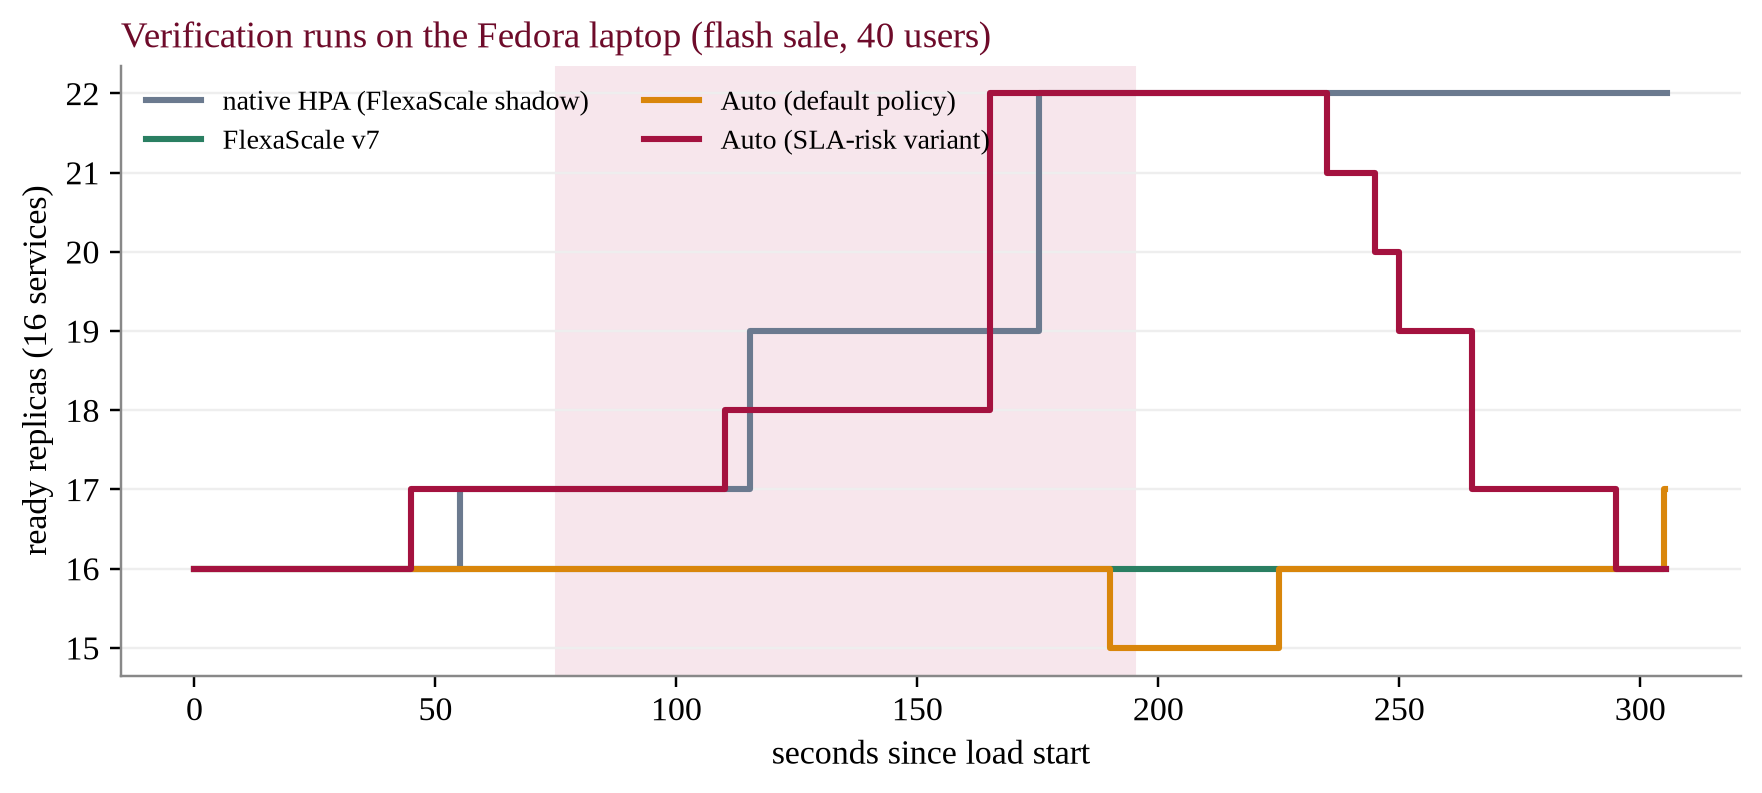
\includegraphics[width=0.8\textwidth]{figures/fig_verification.png}
\caption{Total~ready~replicas~in~four~verification~runs}\label{fig:verify}
\end{figure}

\begin{figure}[!htbp]\centering
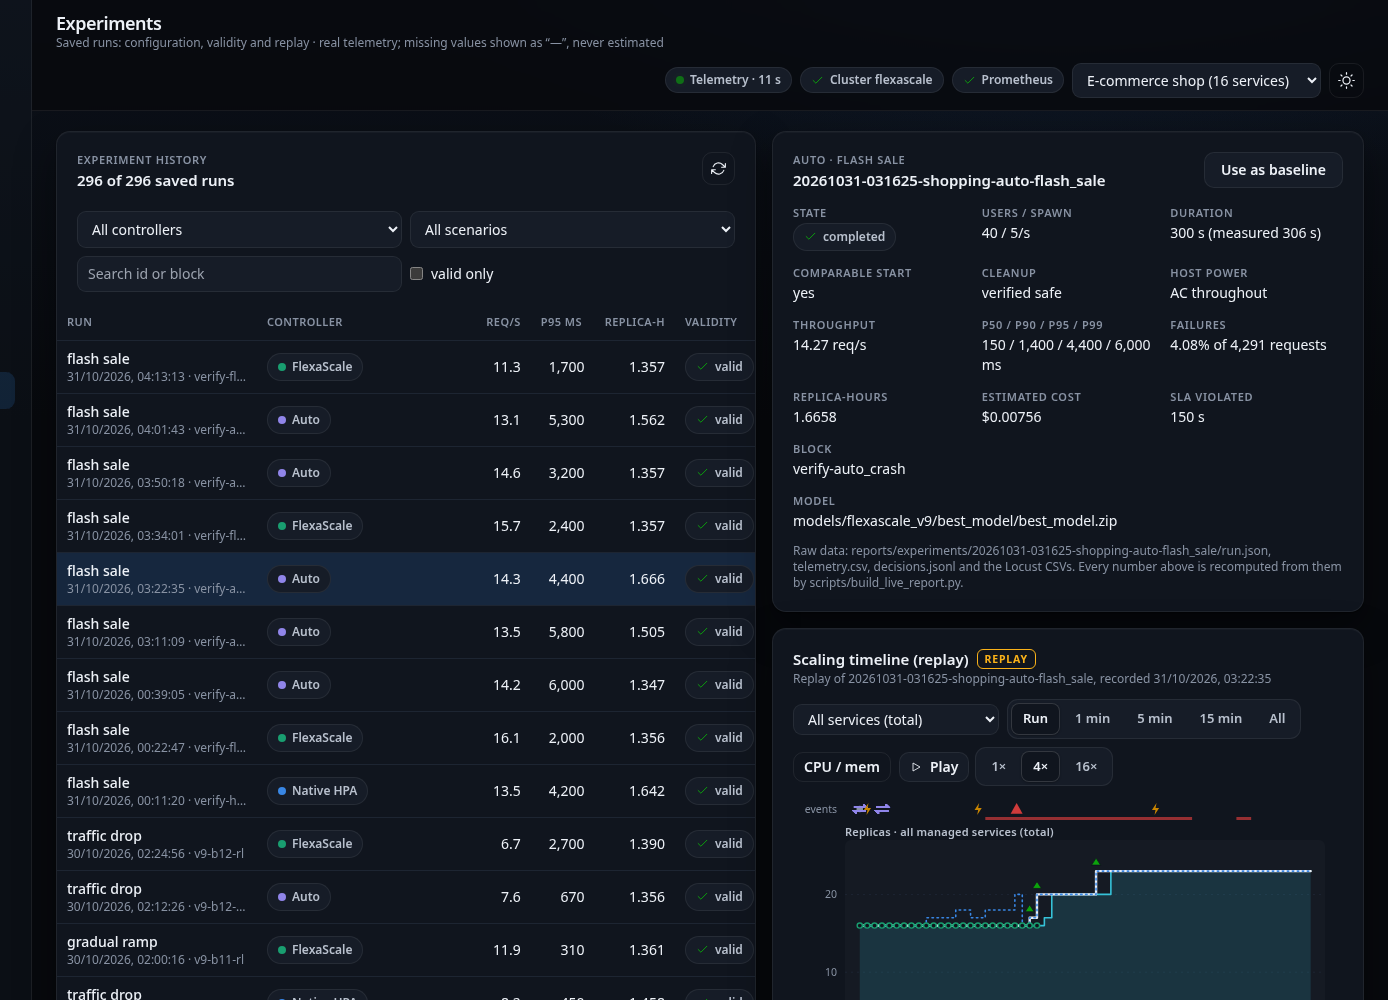
\includegraphics[width=0.75\textwidth]{figures/shot_crash.png}
\caption{Dashboard~replay~of~the~operator-kill~run:~the~fallback~marker~and~HPA~scaling~afterwards}\label{fig:crash}
\end{figure}

\textbf{Pure~FlexaScale~mode.}~In~the~three~FlexaScale-mode~runs~on~this~laptop,~ownership,~safety~and~execution~worked,~but~the~policies~proposed~no~change:~both~v7~and~v9~held~every~service~at~one~replica,~at~40~users~and~at~25~users.~The~reason~is~examined~in~Section~6.5.~Scale~changes~in~FlexaScale~mode~had~been~verified~on~the~same~laptop~before~(run~20261028-061846:~order~service~1$\rightarrow$2~at~+115~s,~ready~at~+130~s~and~back~to~1~at~+255~s),~and~in~the~v9~evaluation~on~the~second~laptop~(run~E2~below).


\textbf{Other~checks.}~The~automated~test~suite~of~373~tests~passed.~The~Helm~lifecycle~script~installed,~upgraded,~rolled~back~and~uninstalled~the~chart~for~the~bookstore~application~and~passed~all~33~checks;~the~main~release~was~upgraded~from~chart~0.4.1~to~0.5.1,~rolled~back~and~upgraded~again~while~the~shop's~Deployments~and~the~database~volume~were~preserved.~For~every~service,~the~per-service~latency~percentiles~were~computed~from~the~service's~own~histogram~and~window,~and~were~ordered~p50~$\le$~p90~$\le$~p95~$\le$~p99~in~every~sample~checked.


\subsection{Results~in~the~application~twin}

After~the~live~evaluation,~every~controller~was~run~once~on~the~three~held-out~twin~test~sets~of~the~second~laptop~(Table~\ref{tab:twin}).~On~the~six~live~scenarios~(T1),~the~tuned~HPA~scored~best~and~v9~was~very~close.~On~random~variations~of~the~shop's~workloads~(T2),~v9~was~best,~with~the~lowest~SLO-violation~time~among~the~efficient~controllers.~On~random~synthetic~applications~(T3),~all~controllers~struggled,~and~the~learned~policies~traded~fewer~replicas~for~more~scaling~events.


\begingroup\small\setlength{\tabcolsep}{4pt}\renewcommand{\arraystretch}{1.25}
\begin{longtable}{|>{\raggedright\arraybackslash}p{3.53cm}|>{\raggedright\arraybackslash}p{1.14cm}|>{\raggedright\arraybackslash}p{1.01cm}|>{\raggedright\arraybackslash}p{1.01cm}|>{\raggedright\arraybackslash}p{1.26cm}|>{\raggedright\arraybackslash}p{1.01cm}|>{\raggedright\arraybackslash}p{1.01cm}|>{\raggedright\arraybackslash}p{1.39cm}|>{\raggedright\arraybackslash}p{1.26cm}|}
\caption{Held-out~twin~test~results~(episode~reward,~higher~is~better;~replica-hours;~p95~in~ms)}\label{tab:twin}\\\hline
\textbf{Controller} & \textbf{T1~reward} & \textbf{T1~RH} & \textbf{T1~p95} & \textbf{T2~reward} & \textbf{T2~RH} & \textbf{T2~p95} & \textbf{T3~reward} & \textbf{T3~RH}\\\hline\endfirsthead
\hline \textbf{Controller} & \textbf{T1~reward} & \textbf{T1~RH} & \textbf{T1~p95} & \textbf{T2~reward} & \textbf{T2~RH} & \textbf{T2~p95} & \textbf{T3~reward} & \textbf{T3~RH}\\\hline\endhead
Default~HPA~(70\%,~300~s) & $-$6.325 & 1.477 & 168 & $-$15.694 & 2.461 & 167 & $-$109.3 & 3.448\\\hline
Tuned~HPA~(350\%,~60~s) & \textbf{$-$1.196} & 1.333 & 178 & $-$3.060 & 2.071 & 217 & $-$82.4 & 1.673\\\hline
Rule~limit\_target(0.6/0.3) & $-$1.280 & 1.338 & 174 & $-$2.789 & 2.080 & 208 & $-$79.3 & 1.802\\\hline
v9~selected~(focal\_bc\_s2) & $-$1.255 & 1.340 & 171 & \textbf{$-$2.548} & 2.078 & 198 & $-$79.0 & 1.815\\\hline
v9~no~graph~(seed~1) & $-$1.255 & 1.339 & 173 & $-$2.839 & 2.094 & 194 & $-$76.7 & 1.969\\\hline
\end{longtable}\endgroup

The~graph~ablation~compared~the~graph~policy~with~the~same~network~without~message~passing,~trained~with~the~same~seed,~episode~by~episode.~The~difference~in~reward~was~$-$0.001~[$-$0.026,~+0.024]~on~T1,~+0.157~[$-$0.363,~+0.677]~on~T2~and~+0.708~[$-$3.304,~+4.720]~on~T3.~Every~interval~includes~zero,~so~the~graph~input~showed~no~measurable~benefit~on~this~shop.


\subsection{Pre-registered~live~evaluation}

Table~\ref{tab:arms}~and~Figure~\ref{fig:arms}~give~the~mean~of~every~valid~run~per~arm~in~the~v9~evaluation.~FlexaScale~RL~and~Auto~used~the~same~replica-hours~as~the~tuned~HPA~and~about~10\%~fewer~than~the~default~HPA.~Their~median~latency~was~the~lowest,~and~their~tail~latency~the~highest.


\begingroup\small\setlength{\tabcolsep}{4pt}\renewcommand{\arraystretch}{1.25}
\begin{longtable}{|>{\raggedright\arraybackslash}p{2.21cm}|>{\raggedright\arraybackslash}p{0.86cm}|>{\raggedright\arraybackslash}p{1.23cm}|>{\raggedright\arraybackslash}p{1.35cm}|>{\raggedright\arraybackslash}p{0.98cm}|>{\raggedright\arraybackslash}p{0.98cm}|>{\raggedright\arraybackslash}p{0.98cm}|>{\raggedright\arraybackslash}p{1.23cm}|>{\raggedright\arraybackslash}p{0.98cm}|>{\raggedright\arraybackslash}p{1.48cm}|}
\caption{v9~evaluation:~mean~over~valid~runs~per~arm~(second~laptop,~25~users,~300~s)}\label{tab:arms}\\\hline
\textbf{Arm} & \textbf{Runs} & \textbf{Replica-hours} & \textbf{Cost~(USD)} & \textbf{p50~(ms)} & \textbf{p95~(ms)} & \textbf{p99~(ms)} & \textbf{Failures~(\%)} & \textbf{req/s} & \textbf{SLO~violation~(s)}\\\hline\endfirsthead
\hline \textbf{Arm} & \textbf{Runs} & \textbf{Replica-hours} & \textbf{Cost~(USD)} & \textbf{p50~(ms)} & \textbf{p95~(ms)} & \textbf{p99~(ms)} & \textbf{Failures~(\%)} & \textbf{req/s} & \textbf{SLO~violation~(s)}\\\hline\endhead
Default~HPA & 12 & 1.512 & 0.00685 & 44 & 241 & 838 & 0.29 & 15.13 & 22.9\\\hline
Tuned~HPA & 12 & 1.366 & 0.00618 & 42 & 167 & 510 & 0.25 & 15.37 & 8.0\\\hline
FlexaScale~RL & 11 & 1.368 & 0.00619 & 37 & 395 & 1674 & 0.34 & 15.07 & 25.6\\\hline
FlexaScale~Auto & 11 & 1.365 & 0.00618 & 37 & 200 & 1936 & 0.32 & 15.15 & 15.7\\\hline
\end{longtable}\endgroup

\begin{figure}[!htbp]\centering
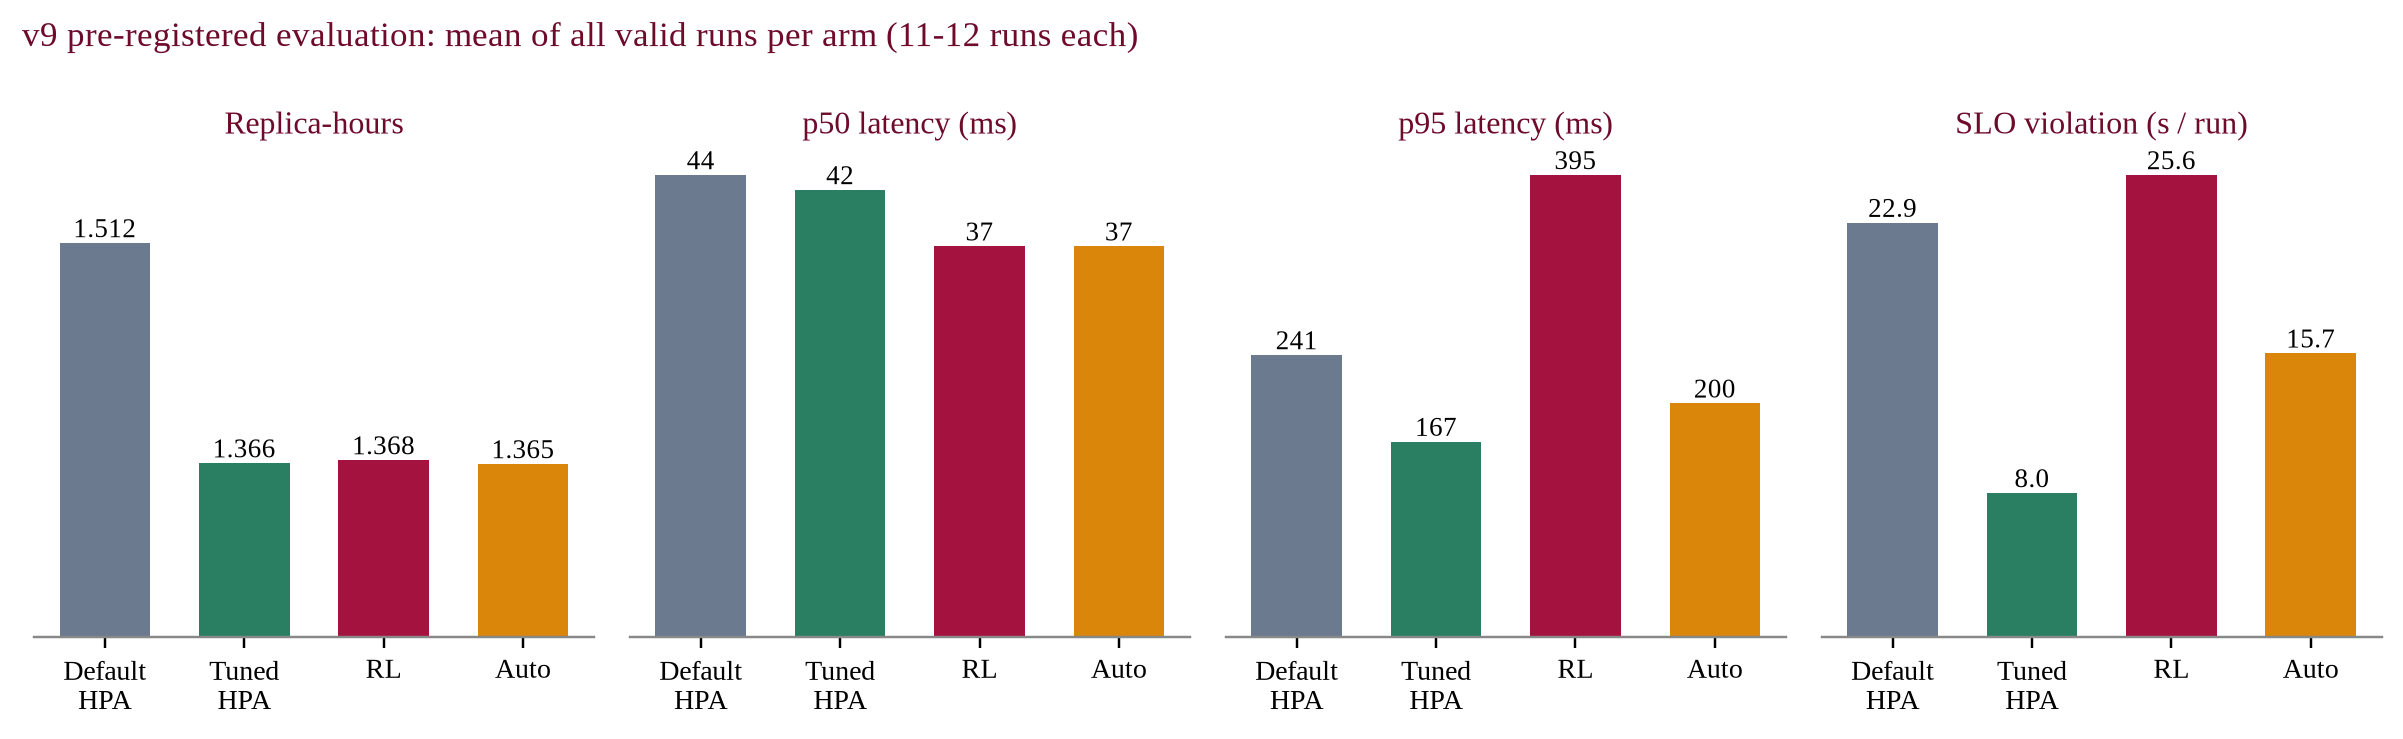
\includegraphics[width=1.0\textwidth]{figures/fig_v9_arms.png}
\caption{v9~evaluation:~replica-hours,~median~and~tail~latency~and~SLO-violation~time~per~arm}\label{fig:arms}
\end{figure}

Table~\ref{tab:pooled}~gives~the~paired~comparisons~with~their~confidence~intervals~and~the~pre-registered~verdicts,~and~Figures~\ref{fig:forest}~and~\ref{fig:forestp95}~show~them~graphically.


\begingroup\small\setlength{\tabcolsep}{4pt}\renewcommand{\arraystretch}{1.25}
\begin{longtable}{|>{\raggedright\arraybackslash}p{1.09cm}|>{\raggedright\arraybackslash}p{3.67cm}|>{\raggedright\arraybackslash}p{0.95cm}|>{\raggedright\arraybackslash}p{2.72cm}|>{\raggedright\arraybackslash}p{2.85cm}|>{\raggedright\arraybackslash}p{2.31cm}|}
\caption{Pre-registered~paired~comparisons~(mean~$\Delta$~with~95\%~CI)}\label{tab:pooled}\\\hline
\textbf{Study} & \textbf{Comparison} & \textbf{Pairs} & \textbf{Replica-hours~$\Delta$} & \textbf{p95~$\Delta$} & \textbf{Verdict}\\\hline\endfirsthead
\hline \textbf{Study} & \textbf{Comparison} & \textbf{Pairs} & \textbf{Replica-hours~$\Delta$} & \textbf{p95~$\Delta$} & \textbf{Verdict}\\\hline\endhead
v9 & Tuned~HPA~vs~default~HPA & 12 & \textbf{$-$9.0\%}~[$-$13.9,~$-$4.1] & $-$10.7\%~[$-$27.5,~+6.1] & Beats~on~cost\\\hline
v9 & FlexaScale~RL~vs~default~HPA & 11 & \textbf{$-$7.3\%}~[$-$11.5,~$-$3.2] & +53.5\%~[$-$49.4,~+156.4] & On~par~/~inconclusive\\\hline
v9 & FlexaScale~Auto~vs~default~HPA & 11 & \textbf{$-$7.7\%}~[$-$12.3,~$-$3.2] & +17.6\%~[$-$6.0,~+41.2] & On~par~/~inconclusive\\\hline
v9 & FlexaScale~RL~vs~tuned~HPA & 11 & +0.3\%~[$-$0.2,~+0.7] & +155\%~[$-$165,~+475] & On~par~/~inconclusive\\\hline
v9 & FlexaScale~Auto~vs~tuned~HPA & 11 & +0.2\%~[$-$0.2,~+0.5] & +41.5\%~[$-$22.6,~+105.7] & On~par~/~inconclusive\\\hline
v7 & FlexaScale~RL~vs~tuned~HPA & 12 & +0.1\%~[$-$0.1,~+0.2] & +7.2\%~[$-$8.1,~+22.4] & On~par~/~inconclusive\\\hline
v7 & FlexaScale~Auto~vs~tuned~HPA & 12 & +0.1\%~[$-$0.1,~+0.2] & +0.1\%~[$-$9.3,~+9.5] & On~par~/~inconclusive\\\hline
v7 & Rule~(no~model)~vs~tuned~HPA & 12 & $-$0.0\%~[$-$0.1,~+0.0] & +4.5\%~[$-$6.6,~+15.6] & On~par~/~inconclusive\\\hline
\end{longtable}\endgroup

\begin{figure}[!htbp]\centering
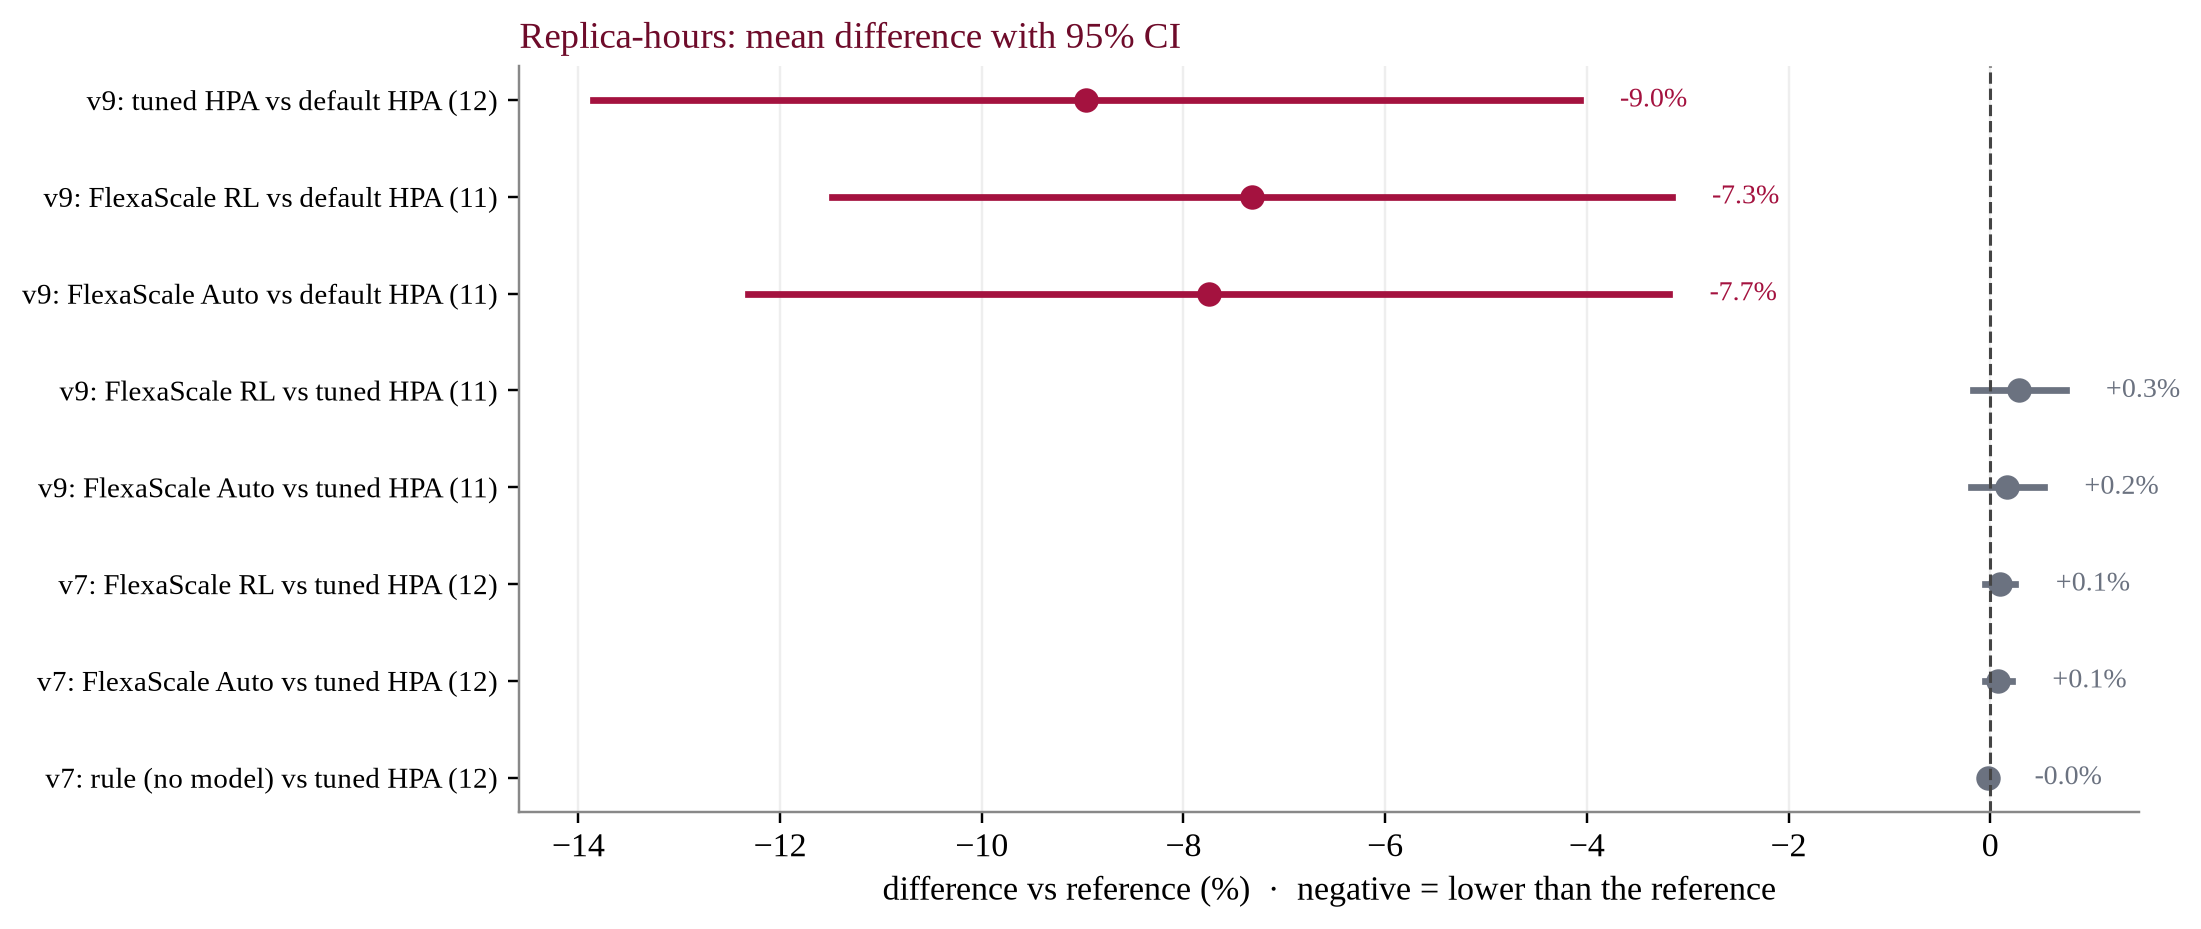
\includegraphics[width=0.88\textwidth]{figures/fig_forest_replica_hours.png}
\caption{Replica-hours:~paired~differences~with~95\%~confidence~intervals}\label{fig:forest}
\end{figure}

\begin{figure}[!htbp]\centering
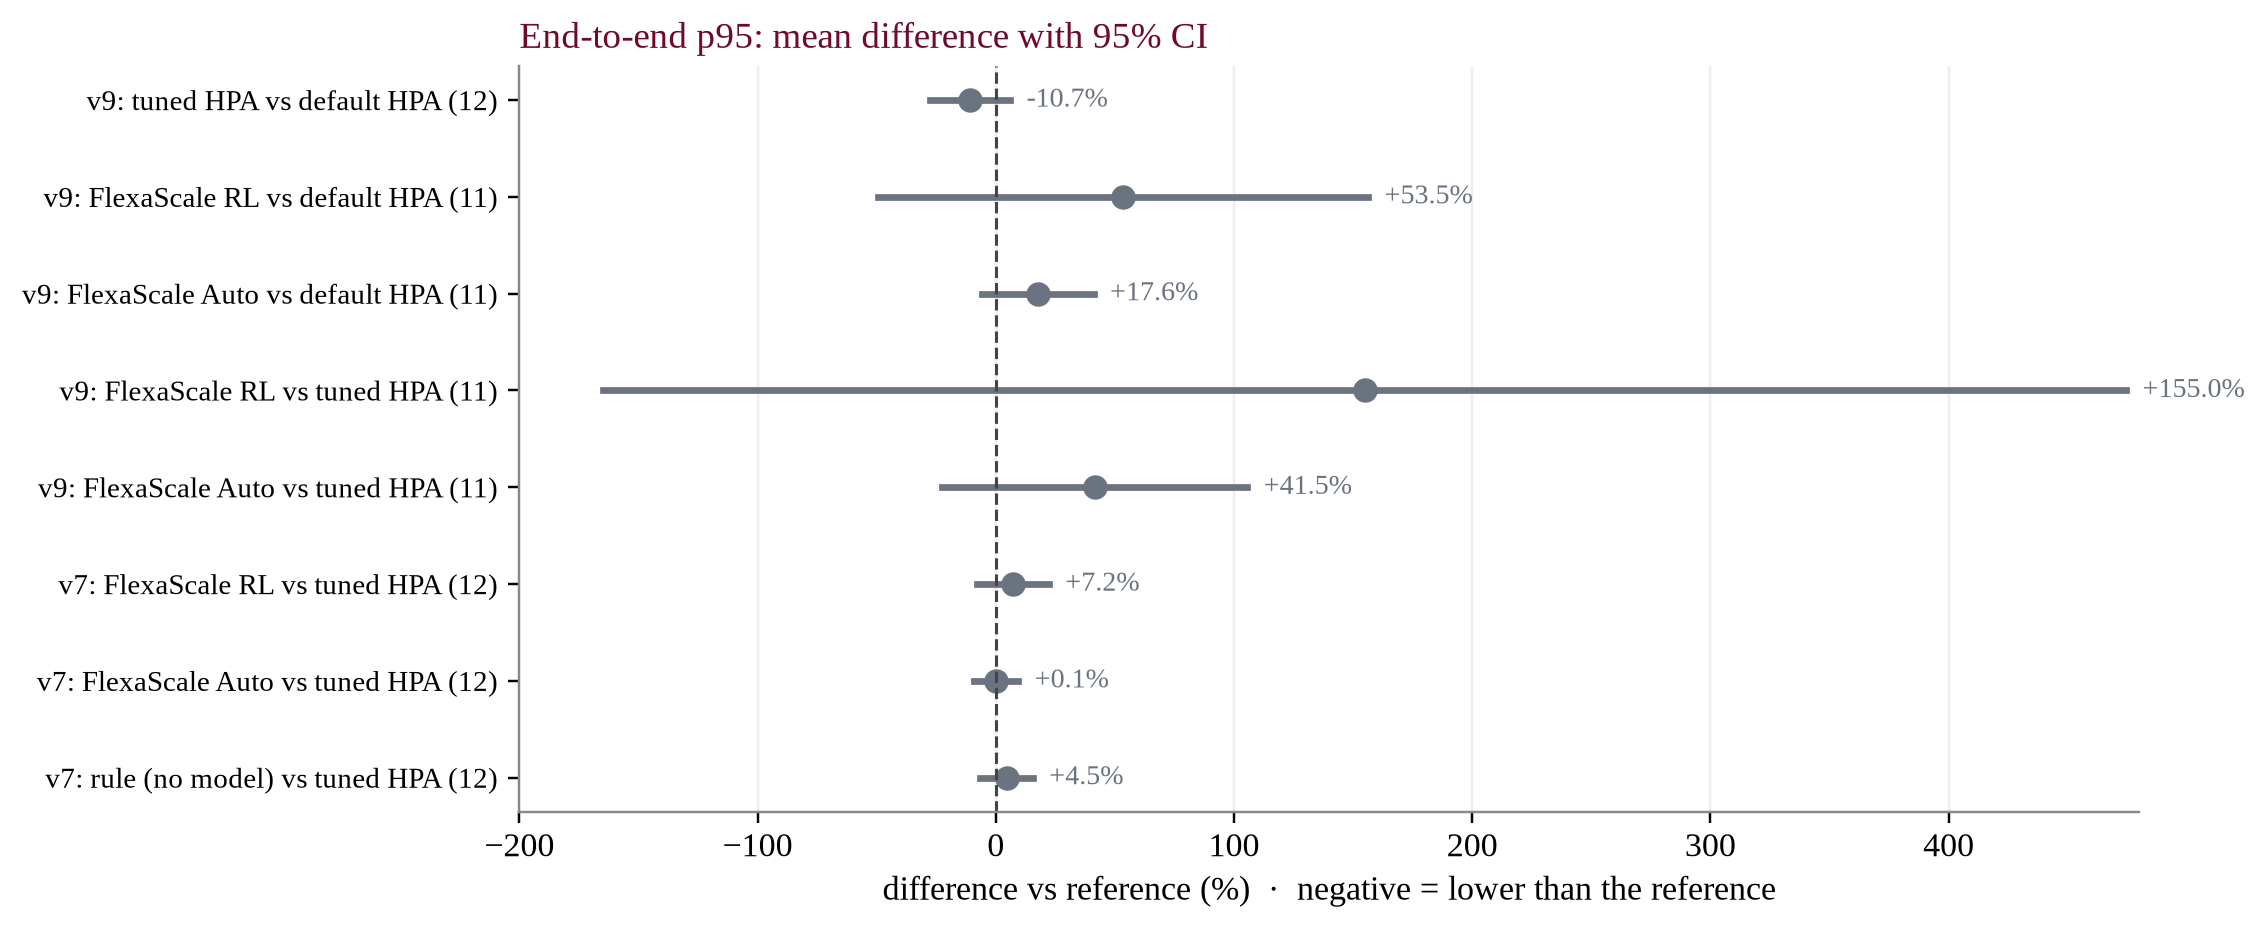
\includegraphics[width=0.88\textwidth]{figures/fig_forest_p95.png}
\caption{End-to-end~p95~latency:~paired~differences~with~95\%~confidence~intervals}\label{fig:forestp95}
\end{figure}

The~p95~means~of~the~FlexaScale~arms~are~strongly~affected~by~three~late~reruns~that~ran~one~to~two~hours~after~their~blocks~while~the~laptop~was~short~of~physical~memory.~Excluding~the~pairs~that~contain~them,~as~a~descriptive~sensitivity~check~only,~FlexaScale~RL~against~the~tuned~HPA~was~+0.1\%~in~replica-hours~and~+3.8\%~[$-$6.2,~+13.9]~in~p95.~The~verdicts~do~not~change.


\subsection{Case~studies:~flash~sale~and~checkout-heavy~load}

Four~blocks~of~the~v9~evaluation~show~where~FlexaScale~saves~resources.~They~were~selected~because~a~FlexaScale~arm~did~better~than~the~default~HPA~on~a~clearly~defined~measure,~so~they~illustrate~the~mechanism;~the~pooled~results~above,~not~these~cases,~are~the~evidence~for~or~against~an~overall~advantage.


\begingroup\small\setlength{\tabcolsep}{4pt}\renewcommand{\arraystretch}{1.25}
\begin{longtable}{|>{\raggedright\arraybackslash}p{2.92cm}|>{\raggedright\arraybackslash}p{1.72cm}|>{\raggedright\arraybackslash}p{1.72cm}|>{\raggedright\arraybackslash}p{1.72cm}|>{\raggedright\arraybackslash}p{1.72cm}|>{\raggedright\arraybackslash}p{1.72cm}|>{\raggedright\arraybackslash}p{1.72cm}|}
\caption{E1:~flash~sale,~v9~block~4~(Auto)~and~E2:~flash~sale,~v9~block~10~(RL)}\label{tab:e1}\\\hline
\textbf{Measure} & \textbf{E1~default~HPA} & \textbf{E1~tuned~HPA} & \textbf{E1~Auto} & \textbf{E2~default~HPA} & \textbf{E2~tuned~HPA} & \textbf{E2~RL}\\\hline\endfirsthead
\hline \textbf{Measure} & \textbf{E1~default~HPA} & \textbf{E1~tuned~HPA} & \textbf{E1~Auto} & \textbf{E2~default~HPA} & \textbf{E2~tuned~HPA} & \textbf{E2~RL}\\\hline\endhead
Throughput~(req/s) & 15.62 & 16.15 & \textbf{16.95} & 13.36 & 15.24 & 15.12\\\hline
p50~/~p95~(ms) & 130~/~410 & 120~/~320 & 130~/~\textbf{200} & 140~/~930 & 130~/~400 & 130~/~\textbf{330}\\\hline
p99~(ms) & 1300 & 470 & 340 & 3200 & 760 & 1400\\\hline
Error~rate~(\%) & 0.30 & 0.43 & 0.35 & 0.92 & 0.37 & 0.37\\\hline
Average~/~peak~replicas & 22.2~/~27 & 16.3~/~17 & 16.6~/~17 & 21.4~/~28 & 16.5~/~17 & 16.6~/~17\\\hline
Replica-hours & 1.829 & 1.386 & \textbf{1.410} & 1.766 & 1.398 & \textbf{1.412}\\\hline
SLO~violation~(s) & 30 & 0 & \textbf{0} & 115 & 5 & 30.1\\\hline
Scaling~events & 8 & 2 & 2 & 10 & 1 & 2\\\hline
\end{longtable}\endgroup

In~E1~the~default~HPA~reacted~to~the~spike~after~it~had~started,~reached~27~replicas~and~kept~them~for~five~minutes~after~the~spike~ended,~and~it~still~spent~30~seconds~above~the~SLO.~Auto,~with~the~v9~policy~owning~the~services,~added~one~replica~where~it~was~needed~and~held~the~rest:~22.9\%~fewer~replica-hours,~p95~halved~($-$51.2\%)~and~no~SLO~violation~(Figure~\ref{fig:e1}).~E2~repeated~the~pattern~in~an~independent~block~with~the~pure~learned~policy:~20.1\%~fewer~replica-hours~and~p95~$-$64.5\%.~In~both~blocks,~however,~the~tuned~HPA~achieved~almost~the~same~replica-hours,~with~less~SLO-violation~time~in~E2.


\begin{figure}[!htbp]\centering
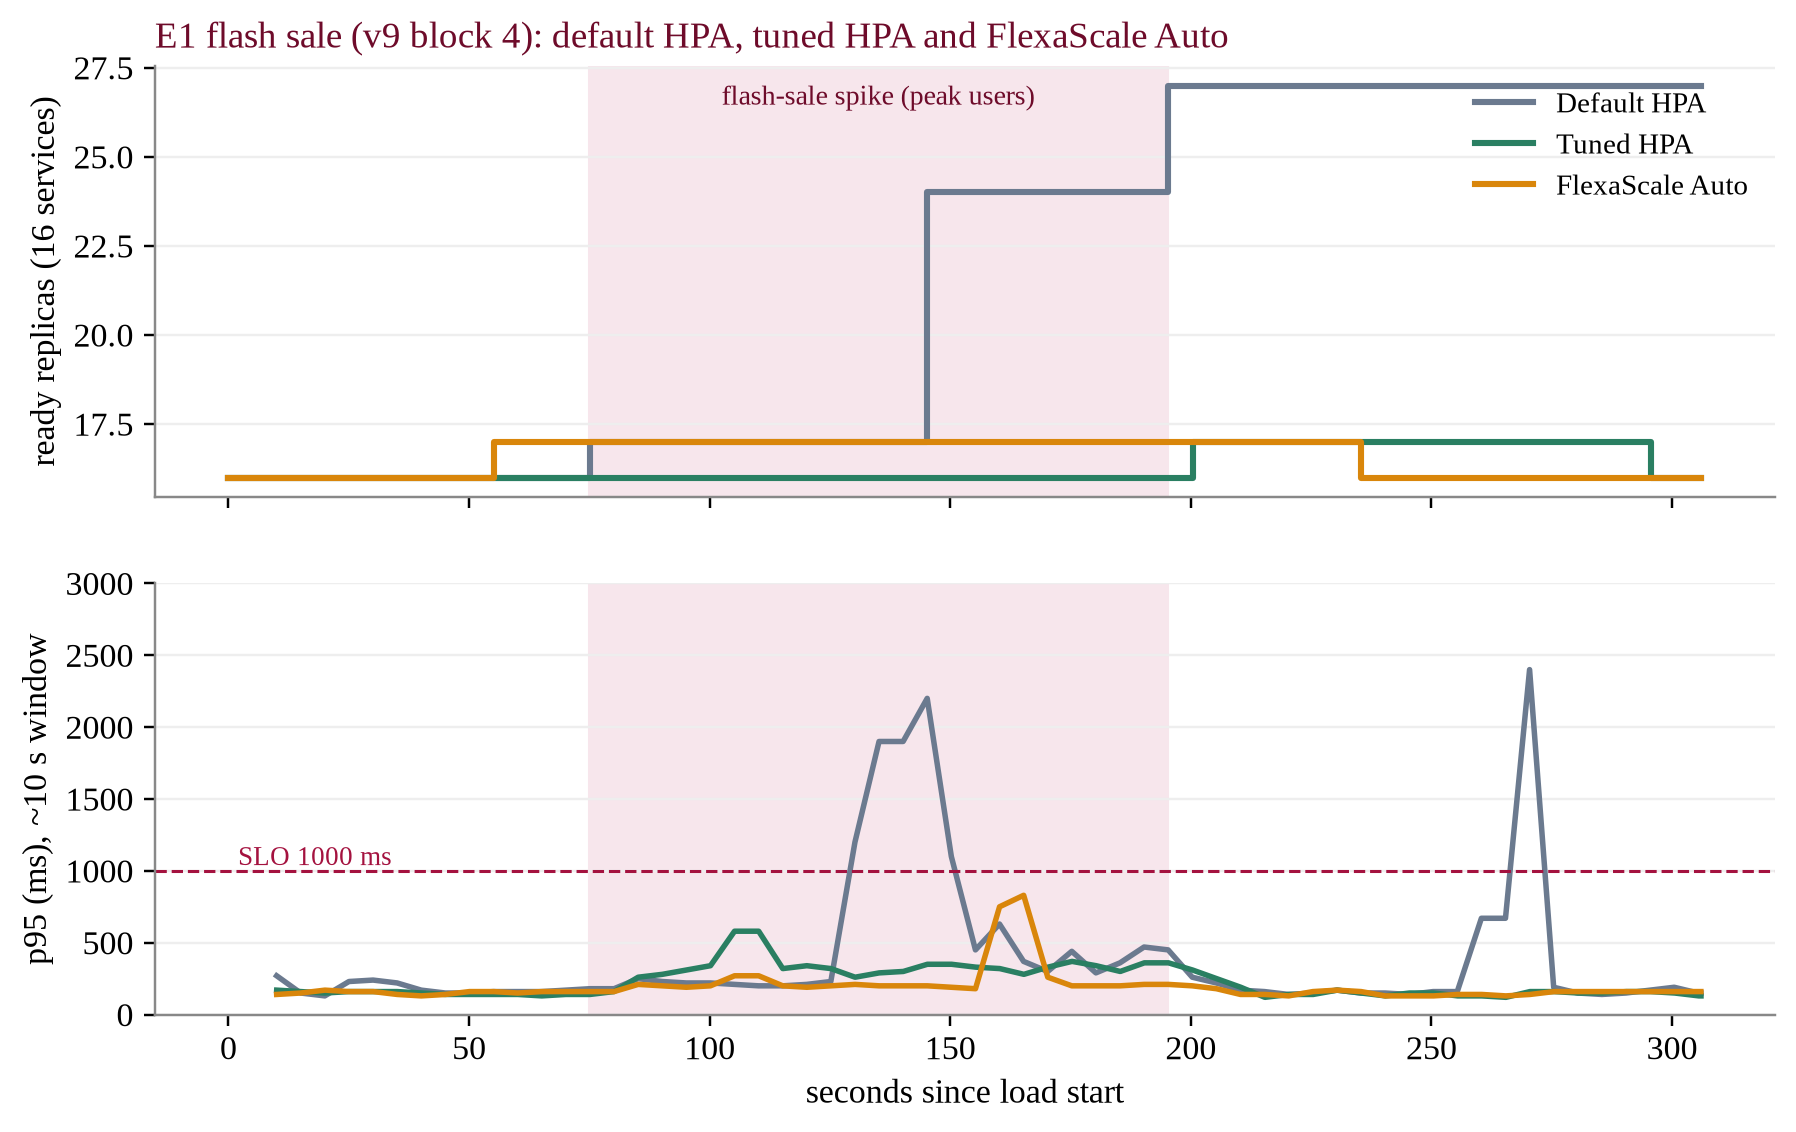
\includegraphics[width=0.9\textwidth]{figures/fig_e1.png}
\caption{E1~flash~sale:~total~ready~replicas~and~end-to-end~p95~under~default~HPA,~tuned~HPA~and~Auto}\label{fig:e1}
\end{figure}

In~the~checkout-heavy~blocks~E3~and~E4,~the~default~HPA~scaled~three~or~four~services~to~two~replicas~for~a~CPU~signal~that~did~not~need~them,~while~FlexaScale~(RL~and~Auto)~and~the~tuned~HPA~held~every~service~at~one~replica.~FlexaScale~used~15.3\%~and~13.8\%~fewer~replica-hours~than~the~default~HPA,~at~the~cost~of~a~p95~about~6\%~higher~(170~against~160~ms,~190~against~180~ms),~which~is~at~the~resolution~of~Locust's~percentile~buckets.


\subsection{Dashboard~outputs}

The~control~center~makes~every~decision~visible~while~it~happens~and~afterwards.~Figure~\ref{fig:livelab}~shows~the~Live~lab~during~an~Auto~experiment~and~Figure~\ref{fig:autopage}~the~Auto~mode~page~after~the~SLA-risk~run,~with~the~owner~band,~hand-off~markers,~rule~usage~(SLA~risk~7\%,~efficiency~93\%)~and~each~service's~owner~and~reason.


\begin{figure}[!htbp]\centering
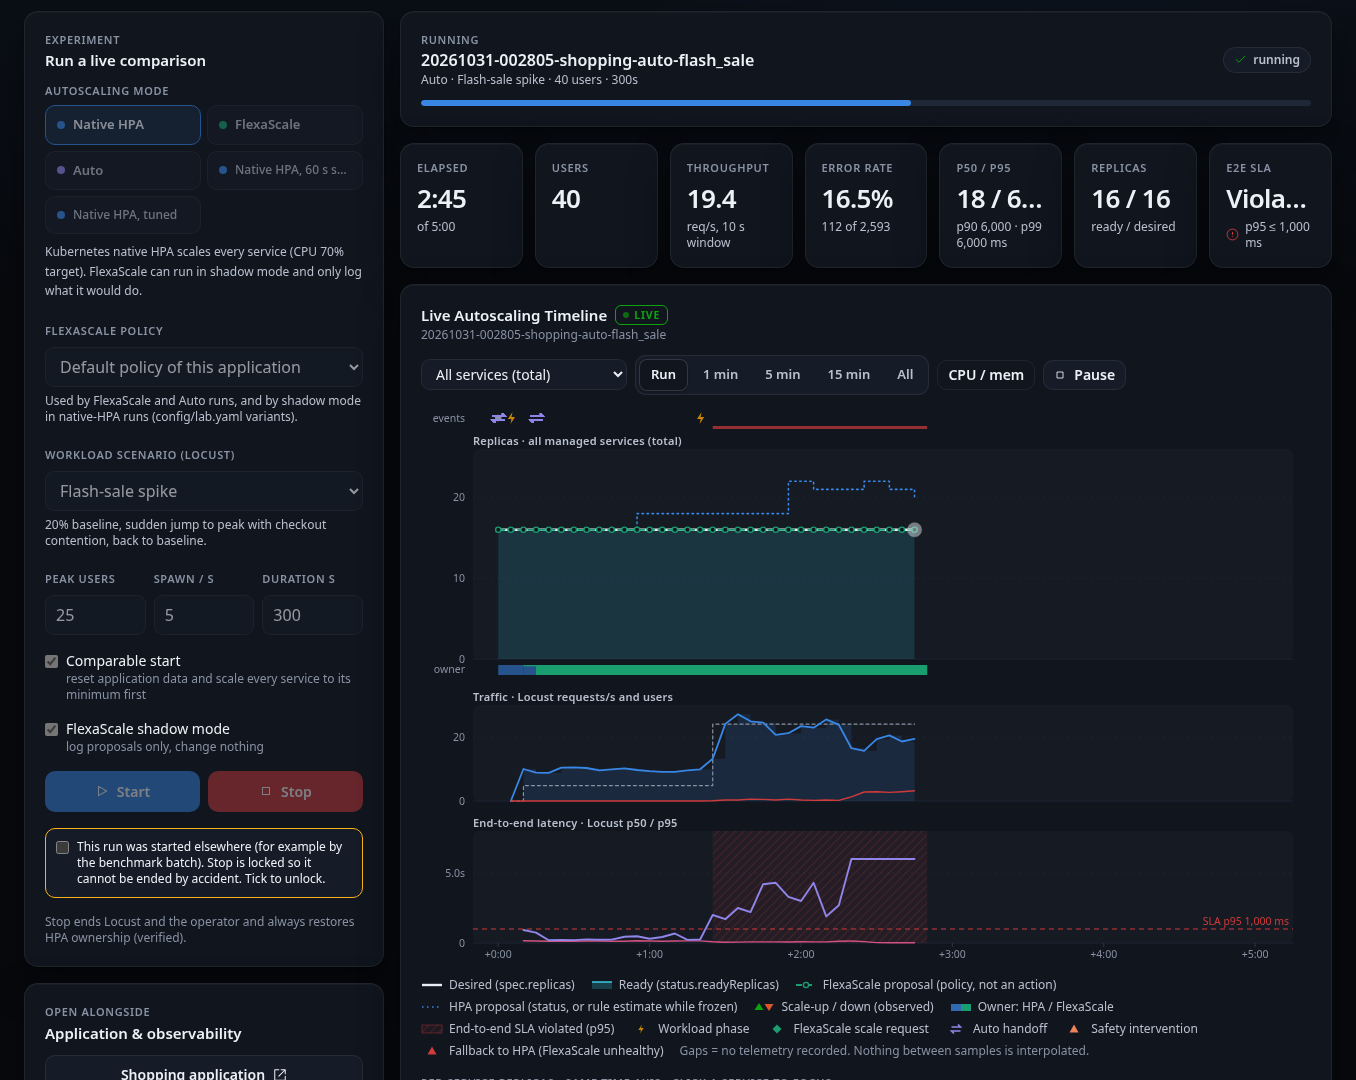
\includegraphics[width=0.88\textwidth]{figures/shot_live_lab.png}
\caption{Live~lab~during~an~Auto-mode~flash-sale~run:~tiles,~live~autoscaling~timeline~and~per-service~replicas}\label{fig:livelab}
\end{figure}

\begin{figure}[!htbp]\centering
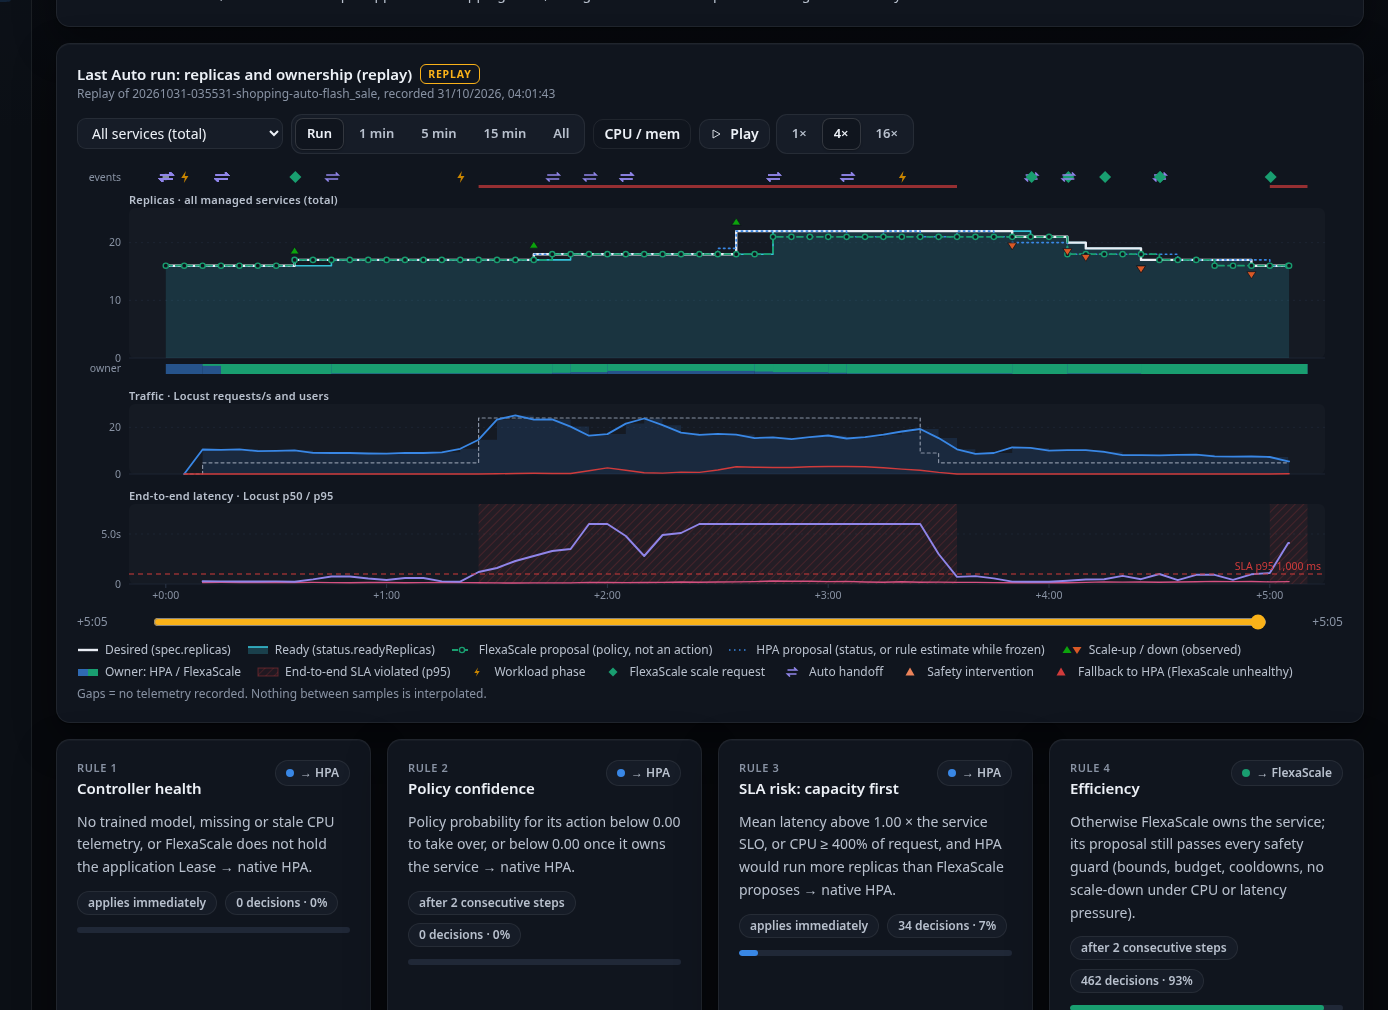
\includegraphics[width=0.88\textwidth]{figures/shot_auto_page.png}
\caption{Auto~mode~page:~replay~of~the~SLA-risk~run~and~the~four~rules~with~their~usage}\label{fig:autopage}
\end{figure}

\section{Comparative~Analysis}

\textbf{Against~the~default~HPA.}~FlexaScale~used~fewer~resources:~7.3\%~(RL)~and~7.7\%~(Auto)~fewer~replica-hours~with~intervals~entirely~below~zero,~and~an~estimated~cost~lower~by~7.4\%~and~7.9\%.~Figure~\ref{fig:scenario}~shows~where~the~saving~comes~from.~The~flash-sale~and~checkout-heavy~scenarios~carry~it,~because~FlexaScale~did~not~keep~spike~capacity~for~the~HPA's~five-minute~window~and~did~not~react~to~brief~CPU~rises.~In~gradual~ramp~and~traffic~drop,~Auto's~p95~was~30-65\%~higher,~which~is~why~the~p95~check~(C2)~failed~and~the~pre-registered~verdict~is~\textit{on~par~/~inconclusive}~rather~than~\textit{beats~on~cost}.


\begin{figure}[!htbp]\centering
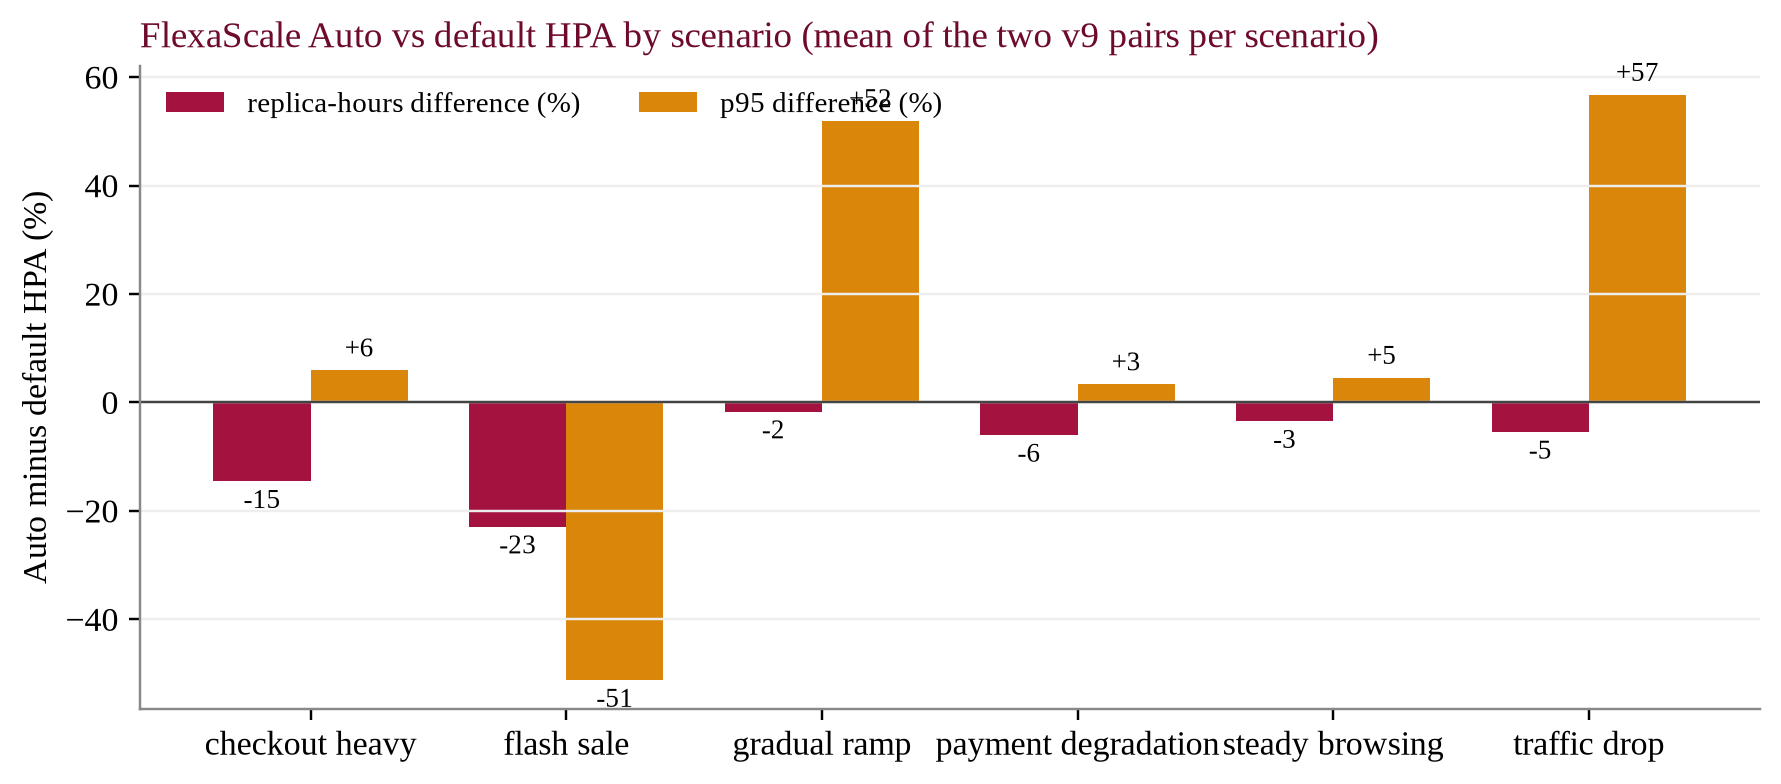
\includegraphics[width=0.85\textwidth]{figures/fig_by_scenario.png}
\caption{FlexaScale~Auto~minus~default~HPA,~by~scenario}\label{fig:scenario}
\end{figure}

\textbf{Against~a~tuned~HPA.}~In~both~pre-registered~studies,~on~two~different~laptops,~FlexaScale~was~on~par:~replica-hours~within~half~a~percent~and~p95~intervals~that~include~zero.~A~tuned~HPA~achieved~the~whole~saving~over~the~default~HPA~without~any~learned~model~($-$9.0\%~replica-hours).~The~v7~study~also~ran~a~hand-written~rule~inside~the~same~operator,~and~it~too~was~on~par,~which~suggests~that~at~these~loads~the~operator's~guards~and~a~sensible~threshold~do~most~of~the~work.


\textbf{Against~the~literature.}~The~systems~reviewed~in~Chapter~3~report~larger~gains:~for~example,~FIRM~reports~up~to~16~times~fewer~SLO~violations~\cite{firm},~and~Gwydion~and~Smart~HPA~report~better~efficiency~than~the~HPA~\cite{gwydion,smarthpa}.~These~figures~are~not~directly~comparable~with~ours:~they~come~from~other~applications,~other~hardware~and,~in~most~cases,~a~comparison~with~the~default~HPA~only.~Against~the~default~HPA,~our~result~points~the~same~way~(a~7-8\%~saving~and~up~to~23\%~in~a~flash~sale).~What~this~project~adds~is~the~comparison~with~a~calibrated~HPA~under~rules~fixed~in~advance,~and~there~the~advantage~disappears.~Table~\ref{tab:compare}~places~FlexaScale~beside~the~closest~related~systems~on~the~design~questions~of~Section~2.2.


\begingroup\small\setlength{\tabcolsep}{4pt}\renewcommand{\arraystretch}{1.25}
\begin{longtable}{|>{\raggedright\arraybackslash}p{2.78cm}|>{\raggedright\arraybackslash}p{2.50cm}|>{\raggedright\arraybackslash}p{2.50cm}|>{\raggedright\arraybackslash}p{2.78cm}|>{\raggedright\arraybackslash}p{3.34cm}|}
\caption{FlexaScale~compared~with~the~closest~related~systems}\label{tab:compare}\\\hline
\textbf{Aspect} & \textbf{Gwydion~\cite{gwydion}} & \textbf{FIRM~\cite{firm}} & \textbf{GRAF~\cite{graf}} & \textbf{FlexaScale}\\\hline\endfirsthead
\hline \textbf{Aspect} & \textbf{Gwydion~\cite{gwydion}} & \textbf{FIRM~\cite{firm}} & \textbf{GRAF~\cite{graf}} & \textbf{FlexaScale}\\\hline\endhead
Decision & Replicas~(RL) & Resource~limits~(RL) & CPU~allocation~(GNN~+~optimiser) & Replicas~(GNN~+~PPO)\\\hline
Dependencies & In~the~state & Critical-path~localisation & GNN~latency~model & Message~passing~on~the~call~graph\\\hline
Coexistence~with~HPA & Not~reported & Not~addressed & Not~addressed & Per-service~Auto~arbitration,~HPA~freeze,~Lease\\\hline
Failure~fallback & Not~reported & Not~reported & Not~reported & Verified:~telemetry~loss,~crash,~Lease~loss\\\hline
Baseline & Default~HPA & Kubernetes~autoscaling & Existing~autoscalers & Default~and~tuned~HPA\\\hline
Evaluation~rules & Not~reported & Not~reported & Not~reported & Pre-registered,~paired,~95\%~CI\\\hline
\end{longtable}\endgroup

\section{Discussion~and~Interpretation}

The~objectives~of~Section~1.2~were~met~as~a~system:~FlexaScale~discovers~and~controls~applications~it~was~not~written~for~(O1),~runs~a~trained~dependency-aware~policy~live~(O2,~O3),~keeps~the~cluster~safe~and~hands~control~back~to~the~HPA~whenever~it~should~(O4),~was~evaluated~fairly~against~both~HPA~configurations~(O5),~and~can~be~watched~and~operated~through~its~dashboard~and~installed~with~Helm~(O6).~The~open~question~was~whether~the~learned~policy~is~a~\textit{better}~controller,~and~the~answer~from~two~independent~studies~is~that~it~is~as~good~as~a~tuned~HPA,~not~better,~on~this~application~and~at~these~loads.


Several~findings~explain~why.~At~25~users,~most~services~sit~at~their~minimum~of~one~replica~under~any~sensible~controller:~the~floor~of~1.333~replica-hours~is~within~2-6\%~of~what~both~the~tuned~HPA~and~FlexaScale~used,~so~there~was~little~left~to~save.~A~tuned~HPA,~with~a~higher~target~and~a~short~scale-down~window,~already~removes~the~default~HPA's~main~sources~of~waste.~The~graph~input~did~not~help~measurably,~probably~because~in~this~shop~the~load~on~each~service~is~visible~in~its~own~request-rate~and~CPU~features~soon~enough,~and~the~twin's~error~in~p95~(about~9\%)~is~of~the~same~size~as~the~differences~the~policy~would~need~to~exploit.


The~verification~runs~revealed~a~more~instructive~limitation.~At~40~users~on~the~first~laptop,~the~order~service's~latency~rose~about~tenfold~while~its~CPU~stayed~at~30-50\%~of~its~limit,~because~it~waits~on~synchronous~database~calls.~Both~learned~policies~rely~mainly~on~CPU~relative~to~the~limit,~so~they~held~one~replica.~The~default~HPA,~whose~target~of~70\%~of~the~request~is~only~14\%~of~the~limit,~added~replicas.~In~Auto~mode,~the~default~SLA-risk~threshold,~calibrated~on~the~second~laptop,~did~not~hand~these~services~to~the~HPA,~and~the~shop's~policy~had~no~per-service~latency~SLO;~with~the~controlled~threshold~it~did.~An~autoscaler~is~only~as~good~as~the~signal~it~reads~and~the~thresholds~calibrated~for~the~machine~it~runs~on,~and~making~Auto~use~end-to-end~latency~directly~is~the~most~useful~improvement~this~points~to.


The~safety~design,~on~the~other~hand,~worked~in~every~case~that~was~tested,~including~the~failures.~This~matters~for~the~practical~goal~of~the~project~and~for~SDG~9:~an~operator~can~let~FlexaScale~manage~services~it~handles~well,~keep~the~HPA~in~charge~of~the~others,~and~rely~on~the~fallback~when~anything~goes~wrong.~The~resource~saving~over~the~default~HPA~is~real~and~statistically~supported,~which~is~the~demonstrated~contribution~to~SDG~12,~but~the~same~saving~is~available~from~tuning~the~HPA,~and~that~should~be~said~plainly.


\section{Limitations}

\begin{itemize}\setlength{\itemsep}{1pt}
  \item \textbf{Scale.}~Single-node~Minikube~on~laptops,~25~to~40~users~and~300-second~runs.~Results~may~differ~on~multi-node~clusters,~under~heavier~load~or~over~longer~periods.
  \item \textbf{One~main~application.}~The~shop~(16~services)~is~the~only~application~evaluated~for~performance;~the~bookstore~was~used~for~deployment~tests~only.
  \item \textbf{Host~noise.}~Laptop~power~profiles,~memory~pressure~and~background~activity~affect~latency.~Validity~rules~controlled~this,~and~seven~runs~were~excluded,~but~the~variance~between~repetitions~remains~large~(tens~of~percent~in~p95).
  \item \textbf{Per-laptop~calibration.}~Thresholds~and~twins~fitted~on~one~laptop~did~not~transfer~to~the~other;~the~v9~policy~is~the~right~one~for~the~second~laptop~and~v7~for~the~first.
  \item \textbf{Signal.}~The~policies~read~mainly~CPU.~Bottlenecks~that~are~not~CPU,~such~as~database~waits,~are~seen~only~indirectly~through~latency~inflation.
  \item \textbf{Statistics.}~Eleven~or~twelve~pairs~per~comparison;~case~studies~E1~to~E4~are~single~pairs~and~illustrate~rather~than~prove.
  \item \textbf{Cost.}~Costs~are~estimates~from~list~prices~applied~to~allocated~resources,~not~measured~bills~or~energy.
\end{itemize}

\clearpage
\chapter{Conclusion}\label{chap:concl}

\section{Conclusion}

This~project~set~out~to~make~Kubernetes~autoscaling~of~microservices~more~efficient~by~giving~the~decision~to~a~learned,~dependency-aware~policy,~without~giving~up~the~safety~of~the~native~HPA.~FlexaScale~achieves~the~second~part~fully.~It~is~a~working~framework~that~discovers~an~application's~services,~builds~unit-free~features~from~Prometheus~telemetry,~runs~a~graph~neural~network~with~a~PPO~policy~over~the~call~graph,~arbitrates~per~service~between~itself~and~the~HPA,~bounds~every~change~with~a~safety~layer,~and~enforces~exclusive~ownership~with~a~Lease~and~an~HPA~freeze.~Live~verification~showed~Auto~mode~selecting~FlexaScale~and~applying~scaling~that~Kubernetes~confirmed,~mixed~ownership~under~SLA~risk,~and~correct~hand-back~to~the~HPA~when~telemetry~was~cut~or~the~operator~was~killed.~The~system~is~tested~by~373~automated~tests,~packaged~as~a~Helm~chart~and~observable~through~a~seven-page~dashboard.


On~the~first~part,~the~evidence~is~mixed~and~was~reported~as~it~came.~In~a~pre-registered~evaluation~of~46~valid~runs,~FlexaScale~used~7.3-7.7\%~fewer~replica-hours~than~the~default~HPA,~with~up~to~23\%~in~a~flash~sale,~but~it~was~on~par~with~a~tuned~HPA~in~two~independent~studies,~and~the~graph~input~showed~no~measurable~benefit.~The~project's~main~contribution~is~therefore~a~safe,~explainable~and~installable~framework~for~learned~autoscaling,~together~with~an~honest~measurement~of~how~much~a~learned~policy~gains~over~well-configured~rules~at~small~scale:~on~this~application,~nothing~beyond~what~tuning~provides.


\section{Future~work}

The~S8~phase~will~build~on~these~results.~The~following~tasks~are~planned,~each~with~its~dependency~and~the~way~it~will~be~validated.


\begin{enumerate}\setlength{\itemsep}{1pt}
  \item \textbf{Latency-aware~inputs~and~Auto~rules.}~Add~end-to-end~and~per-service~latency~SLOs~to~the~policy's~state~and~to~the~SLA-risk~rule,~so~that~non-CPU~bottlenecks~are~handled.~Validation:~the~40-user~verification~scenario,~where~the~current~policies~held~one~replica.
  \item \textbf{Automatic~per-cluster~calibration.}~Derive~Auto~thresholds~and~the~tuned-HPA~baseline~from~a~short~calibration~run~on~each~new~cluster~instead~of~carrying~them~across~machines.~Validation:~repeat~the~v9~protocol~on~both~laptops.
  \item \textbf{Stronger~baselines.}~Compare~with~per-service~tuned~HPAs,~custom-metric~HPAs~and~a~faster~metrics~resolution,~which~could~close~the~gaps~FlexaScale~shows.
  \item \textbf{Larger~clusters~and~loads.}~Run~on~a~multi-node~cluster~with~heavier~and~longer~workloads,~where~more~services~leave~their~minimum~and~dependency~information~has~more~room~to~help.~This~depends~on~access~to~cloud~credits~or~a~lab~cluster.
  \item \textbf{Safe~online~adaptation.}~Fine-tune~the~policy~from~live~data~in~shadow~mode~only,~and~deploy~a~new~checkpoint~after~it~passes~the~same~gate~and~held-out~tests.
  \item \textbf{Publication~and~dissertation.}~Prepare~a~paper~on~fair~evaluation~of~learned~autoscalers~against~tuned~baselines~for~one~of~the~venues~identified~in~the~initial~submission,~and~complete~the~final~dissertation~and~demonstration.
\end{enumerate}

\clearpage
\renewcommand{\bibname}{References}
\begin{thebibliography}{99}
\phantomsection
\addcontentsline{toc}{chapter}{References}
\setlength{\itemsep}{6pt}
\setlength{\parskip}{0pt}

\bibitem{gwydion}
J.~Santos,~E.~Reppas,~T.~Wauters,~B.~Volckaert,~and~F.~De~Turck,~``Gwydion:~Efficient~auto-scaling~for~complex~containerized~applications~in~Kubernetes~through~reinforcement~learning,''~\textit{J.~Netw.~Comput.~Appl.},~vol.~234,~Art.~no.~104067,~2025,~doi:~10.1016/j.jnca.2024.104067.

\bibitem{smarthpa}
H.~Ahmad,~C.~Treude,~M.~Wagner,~and~C.~Szabo,~``Towards~resource-efficient~reactive~and~proactive~auto-scaling~for~microservice~architectures,''~\textit{J.~Syst.~Softw.},~vol.~225,~Art.~no.~112390,~2025,~doi:~10.1016/j.jss.2025.112390.

\bibitem{pandey}
V.~Pandey,~``Reinforcement~learning-based~autoscaling~for~cost~and~performance~optimization~in~Kubernetes~clusters,''~2025.

\bibitem{adaptscale}
Y.~Shi,~M.~Dong,~W.~Zhang,~L.~Liu,~Y.~Zheng,~L.~Cui,~and~J.~Zhang,~``AdaptScale:~An~adaptive~data~scaling~controller~for~improving~multiple~performance~requirements~in~clouds,''~\textit{Future~Gener.~Comput.~Syst.},~vol.~105,~pp.~814--823,~2020,~doi:~10.1016/j.future.2017.08.034.

\bibitem{kubcg}
G.~El~Haj~Ahmed,~F.~Gil-Castiñeira,~and~E.~Costa-Montenegro,~``KubCG:~A~dynamic~Kubernetes~scheduler~for~heterogeneous~clusters,''~\textit{Softw.~Pract.~Exp.},~vol.~51,~no.~2,~pp.~213--234,~2021,~doi:~10.1002/spe.2898.

\bibitem{rossi}
F.~Rossi,~M.~Nardelli,~and~V.~Cardellini,~``Horizontal~and~vertical~scaling~of~container-based~applications~using~reinforcement~learning,''~in~\textit{Proc.~IEEE~12th~Int.~Conf.~Cloud~Computing~(CLOUD)},~Milan,~Italy,~2019,~pp.~329--338,~doi:~10.1109/CLOUD.2019.00061.

\bibitem{firm}
H.~Qiu,~S.~S.~Banerjee,~S.~Jha,~Z.~T.~Kalbarczyk,~and~R.~K.~Iyer,~``FIRM:~An~intelligent~fine-grained~resource~management~framework~for~SLO-oriented~microservices,''~in~\textit{Proc.~14th~USENIX~Symp.~Operating~Systems~Design~and~Implementation~(OSDI)},~2020,~pp.~805--825.

\bibitem{autopilot}
K.~Rzadca~\textit{et~al.},~``Autopilot:~Workload~autoscaling~at~Google,''~in~\textit{Proc.~15th~European~Conf.~Computer~Systems~(EuroSys)},~Heraklion,~Greece,~2020,~Art.~no.~16,~doi:~10.1145/3342195.3387524.

\bibitem{sinan}
Y.~Zhang,~W.~Hua,~Z.~Zhou,~G.~E.~Suh,~and~C.~Delimitrou,~``Sinan:~ML-based~and~QoS-aware~resource~management~for~cloud~microservices,''~in~\textit{Proc.~26th~ACM~Int.~Conf.~Architectural~Support~for~Programming~Languages~and~Operating~Systems~(ASPLOS)},~2021,~pp.~167--181,~doi:~10.1145/3445814.3446693.

\bibitem{graf}
J.~Park,~B.~Choi,~C.~Lee,~and~D.~Han,~``GRAF:~A~graph~neural~network~based~proactive~resource~allocation~framework~for~SLO-oriented~microservices,''~in~\textit{Proc.~17th~Int.~Conf.~emerging~Networking~EXperiments~and~Technologies~(CoNEXT)},~2021,~pp.~154--167,~doi:~10.1145/3485983.3494866.

\bibitem{alibaba}
S.~Luo~\textit{et~al.},~``Characterizing~microservice~dependency~and~performance:~Alibaba~trace~analysis,''~in~\textit{Proc.~ACM~Symp.~Cloud~Computing~(SoCC)},~Seattle,~WA,~USA,~2021,~pp.~412--426,~doi:~10.1145/3472883.3487003.

\bibitem{deathstar}
Y.~Gan~\textit{et~al.},~``An~open-source~benchmark~suite~for~microservices~and~their~hardware-software~implications~for~cloud~\&~edge~systems,''~in~\textit{Proc.~24th~Int.~Conf.~Architectural~Support~for~Programming~Languages~and~Operating~Systems~(ASPLOS)},~Providence,~RI,~USA,~2019,~pp.~3--18,~doi:~10.1145/3297858.3304013.

\bibitem{ppo}
J.~Schulman,~F.~Wolski,~P.~Dhariwal,~A.~Radford,~and~O.~Klimov,~``Proximal~policy~optimization~algorithms,''~arXiv:1707.06347,~2017.

\bibitem{gae}
J.~Schulman,~P.~Moritz,~S.~Levine,~M.~Jordan,~and~P.~Abbeel,~``High-dimensional~continuous~control~using~generalized~advantage~estimation,''~in~\textit{Proc.~Int.~Conf.~Learning~Representations~(ICLR)},~2016,~arXiv:1506.02438.

\bibitem{sb3}
A.~Raffin,~A.~Hill,~A.~Gleave,~A.~Kanervisto,~M.~Ernestus,~and~N.~Dormann,~``Stable-Baselines3:~Reliable~reinforcement~learning~implementations,''~\textit{J.~Mach.~Learn.~Res.},~vol.~22,~no.~268,~pp.~1--8,~2021.

\bibitem{gcn}
T.~N.~Kipf~and~M.~Welling,~``Semi-supervised~classification~with~graph~convolutional~networks,''~in~\textit{Proc.~Int.~Conf.~Learning~Representations~(ICLR)},~2017,~arXiv:1609.02907.

\bibitem{mpnn}
J.~Gilmer,~S.~S.~Schoenholz,~P.~F.~Riley,~O.~Vinyals,~and~G.~E.~Dahl,~``Neural~message~passing~for~quantum~chemistry,''~in~\textit{Proc.~34th~Int.~Conf.~Machine~Learning~(ICML)},~Sydney,~Australia,~2017,~pp.~1263--1272.

\bibitem{borg}
B.~Burns,~B.~Grant,~D.~Oppenheimer,~E.~Brewer,~and~J.~Wilkes,~``Borg,~Omega,~and~Kubernetes,''~\textit{Commun.~ACM},~vol.~59,~no.~5,~pp.~50--57,~2016,~doi:~10.1145/2890784.

\bibitem{k8shpa}
The~Kubernetes~Authors,~``Horizontal~Pod~Autoscaling,''~Kubernetes~Documentation.~[Online].~Available:~https://kubernetes.io/docs/tasks/run-application/horizontal-pod-autoscale/~(accessed~Oct.~2026).

\bibitem{alibabadata}
Alibaba~Group,~``Alibaba~cluster~trace~program:~cluster-trace-microservices-v2021.''~[Online].~Available:~https://github.com/alibaba/clusterdata~(accessed~Oct.~2026).

\bibitem{un2030}
United~Nations~General~Assembly,~``Transforming~our~world:~The~2030~Agenda~for~Sustainable~Development,''~Resolution~A/RES/70/1,~2015.
\end{thebibliography}
\clearpage
\appendix

\clearpage
\chapter{Source~Code~and~Reproducibility}\label{chap:appendix}

The~complete~source~code,~configuration,~trained~models,~raw~experiment~data~and~analysis~scripts~are~in~the~project~repository~below~(branch~\texttt{main},~commit~\texttt{d8416a2}).~No~passwords,~tokens~or~private~keys~are~stored~in~it;~the~shop's~demo~user~account~exists~only~inside~the~local~cluster.~The~Alibaba~raw~trace~(7.4~GB)~is~not~in~the~repository~and~must~be~downloaded~from~its~public~source;~the~processed~dataset~and~its~provenance~file~are~included.


\begin{verbatim}
https://github.com/ashwinpraveengo/flexascale
\end{verbatim}

\section{Setup~and~execution}

\textbf{Prerequisites:}~Docker,~Minikube,~kubectl,~Helm~3,~Python~3.10~or~later~and~Node.js~(only~to~rebuild~the~dashboard).~\textbf{Installation:}


\begin{verbatim}
git clone https://github.com/ashwinpraveengo/flexascale.git
cd flexascale
python -m venv .venv && . .venv/bin/activate
pip install -r requirements.txt && pip install -e .
./fsctl start    # cluster, monitoring, shop, checks, dashboard
                 # dashboard at http://127.0.0.1:8090/
./fsctl status   # owner of scaling, Lease, model, processes
./fsctl stop     # stop all, restore every HPA, verify no Lease
\end{verbatim}

\textbf{Running~an~experiment.}~In~the~dashboard's~Live~lab,~choose~a~mode~(Native~HPA,~FlexaScale~or~Auto),~a~policy,~a~scenario~and~the~number~of~users,~and~press~Start.~On~the~first~laptop~choose~the~v7~policy;~the~default~v9~policy~was~fitted~to~the~second~laptop.~Results~appear~under~Experiments~and~Comparison~and~are~written~to~\texttt{reports/\allowbreak{}experiments/\allowbreak{}<run~id>/\allowbreak{}}.


\textbf{Reproducing~the~results~and~checks:}


\begin{verbatim}
pytest -q                                   # 373 tests
python scripts/build_results.py            # results/ from raw runs
python scripts/verify_controller_modes.py --report
bash scripts/helm_lifecycle_test.sh        # Helm lifecycle checks
python scripts/train_v7.py --help          # v7/v9 training protocol
\end{verbatim}

\section{Supporting~material}

Table~\ref{tab:repo}~maps~the~repository~to~the~parts~of~this~report,~and~Table~\ref{tab:tests}~lists~the~main~groups~of~automated~tests.


\begingroup\small\setlength{\tabcolsep}{4pt}\renewcommand{\arraystretch}{1.25}
\begin{longtable}{|>{\raggedright\arraybackslash}p{5.20cm}|>{\raggedright\arraybackslash}p{9.66cm}|}
\caption{Repository~map}\label{tab:repo}\\\hline
\textbf{Path} & \textbf{Content}\\\hline\endfirsthead
\hline \textbf{Path} & \textbf{Content}\\\hline\endhead
src/flexascale/operator/ & Operator~(app\_operator.py)~and~Auto~rules~(auto\_mode.py)\\\hline
src/flexascale/rl/ & Features~(features\_v3.py),~graph~policy~(graph\_policy.py),~runtime,~imitation\\\hline
src/flexascale/simulator/ & Alibaba-driven~environments~(v1-v6)~and~the~application~twin~(v7,~v9)\\\hline
src/flexascale/safety/ & HPA~freeze~and~restore,~Lease,~ownership~locks\\\hline
src/flexascale/metrics/,~discovery/ & Prometheus~telemetry~and~service~discovery\\\hline
src/flexascale/lab/ & Lab~server,~experiment~runner,~benchmark~and~comparison\\\hline
dashboard/ & React~and~TypeScript~control~center\\\hline
apps/,~charts/shopping-app/ & The~16-service~shop~and~its~Helm~chart\\\hline
helm/flexascale/ & FlexaScale~Helm~chart~0.5.1\\\hline
config/apps/,~config/twin/ & Application~policies~and~fitted~twins\\\hline
models/ & Trained~policies~v2-v9~with~model~cards\\\hline
reports/,~results/ & Raw~runs,~pre-registered~analyses,~verification,~charts~and~screenshots\\\hline
docs/ & Pre-registrations~(POLICY\_V4-V9),~runbook,~learning~guides\\\hline
\end{longtable}\endgroup

\begingroup\small\setlength{\tabcolsep}{4pt}\renewcommand{\arraystretch}{1.25}
\begin{longtable}{|>{\raggedright\arraybackslash}p{5.65cm}|>{\raggedright\arraybackslash}p{9.21cm}|}
\caption{Main~groups~of~automated~tests~(373~tests~in~total,~all~passing)}\label{tab:tests}\\\hline
\textbf{Test~file} & \textbf{What~it~checks}\\\hline\endfirsthead
\hline \textbf{Test~file} & \textbf{What~it~checks}\\\hline\endhead
test\_auto\_mode.py & Every~Auto~rule,~the~order~of~rules~and~the~two-step~dwell\\\hline
test\_operator.py,~test\_agnostic\_operator.py & Guards,~budget,~Lease~loss,~application-agnostic~discovery\\\hline
test\_safety.py & HPA~freeze~and~restore~from~annotations\\\hline
test\_workload\_metrics.py & Pod-level~CPU~fallback,~double~scraping,~zero~versus~missing,~p90~and~capped~percentiles\\\hline
test\_lab.py & Process~safety,~lab~API,~operator~watchdog,~p90~backfill\\\hline
test\_helm\_chart.py & Chart~rendering,~release-specific~selector,~hand-back~hook\\\hline
test\_hpa\_tuned.py & Tuned-HPA~arm~and~model~tags~across~operating~systems\\\hline
\end{longtable}\endgroup
\end{document}